\documentclass[11pt]{report}
\usepackage[utf8]{inputenc}
\usepackage{lmodern}
\usepackage[T1]{fontenc}
\usepackage{amsmath}
\usepackage{amssymb}
\usepackage{amsthm}
\usepackage{enumitem}
\usepackage[margin=1in]{geometry}
\usepackage{graphicx}
\usepackage{microtype}
\usepackage{hyperref}
\usepackage{bookmark}
\usepackage{footnotebackref}
\hypersetup{
  colorlinks=true,
  linkcolor=blue,
  citecolor=blue,
  urlcolor=blue,
  bookmarksnumbered=true,
  bookmarksopen=true,
  pdftitle={Ordinary Differential Equations Lecture Notes},
  pdfauthor={Dan Romik}
}

\setcounter{tocdepth}{2}
\emergencystretch=3em

\renewcommand{\footnoterule}{\kern-3pt\hrule width \textwidth height 0.4pt\kern2.6pt}

\newsavebox{\fitbox}
\newcommand{\fitwidth}[1]{%
  \sbox\fitbox{#1}%
  \ifdim\wd\fitbox>\linewidth\resizebox{\linewidth}{!}{\usebox\fitbox}\else\usebox\fitbox\fi}

% custom macros carried over from the original lecture-notes preamble
\providecommand{\cal}{\mathcal}
\newcommand{\R}{\mathbb{R}}
\newcommand{\Z}{\mathbb{Z}}
\newcommand{\N}{\mathbb{N}}
\newcommand{\Q}{\mathbb{Q}}
\newcommand{\E}{\mathbb{E}}
\newcommand{\prob}{\mathbf{P}}
\newcommand{\expec}{\mathbf{E}}
\newcommand{\var}{\mathbf{V}}
\newcommand{\cov}{\textrm{Cov}}
\newcommand{\ind}{\mathbf{1}}
\newcommand{\eqdist}{\stackrel{d}{=}}

\theoremstyle{plain}
\newtheorem{thm}{Theorem}[chapter]
\newtheorem{lem}[thm]{Lemma}
\newtheorem{cor}[thm]{Corollary}
\theoremstyle{definition}
\newtheorem{defn}[thm]{Definition}
\newtheorem{example}[thm]{Example}
\newtheorem{xexercise}[thm]{Exercise}

\title{Ordinary Differential Equations Lecture Notes \\ MATH 119B --- Spring 2012}
\author{Dan Romik \\ Department of Mathematics, UC Davis}
\date{February 3, 2026}

\begin{document}
\maketitle
\clearpage
\null\vfill
\begin{center}
\fitwidth{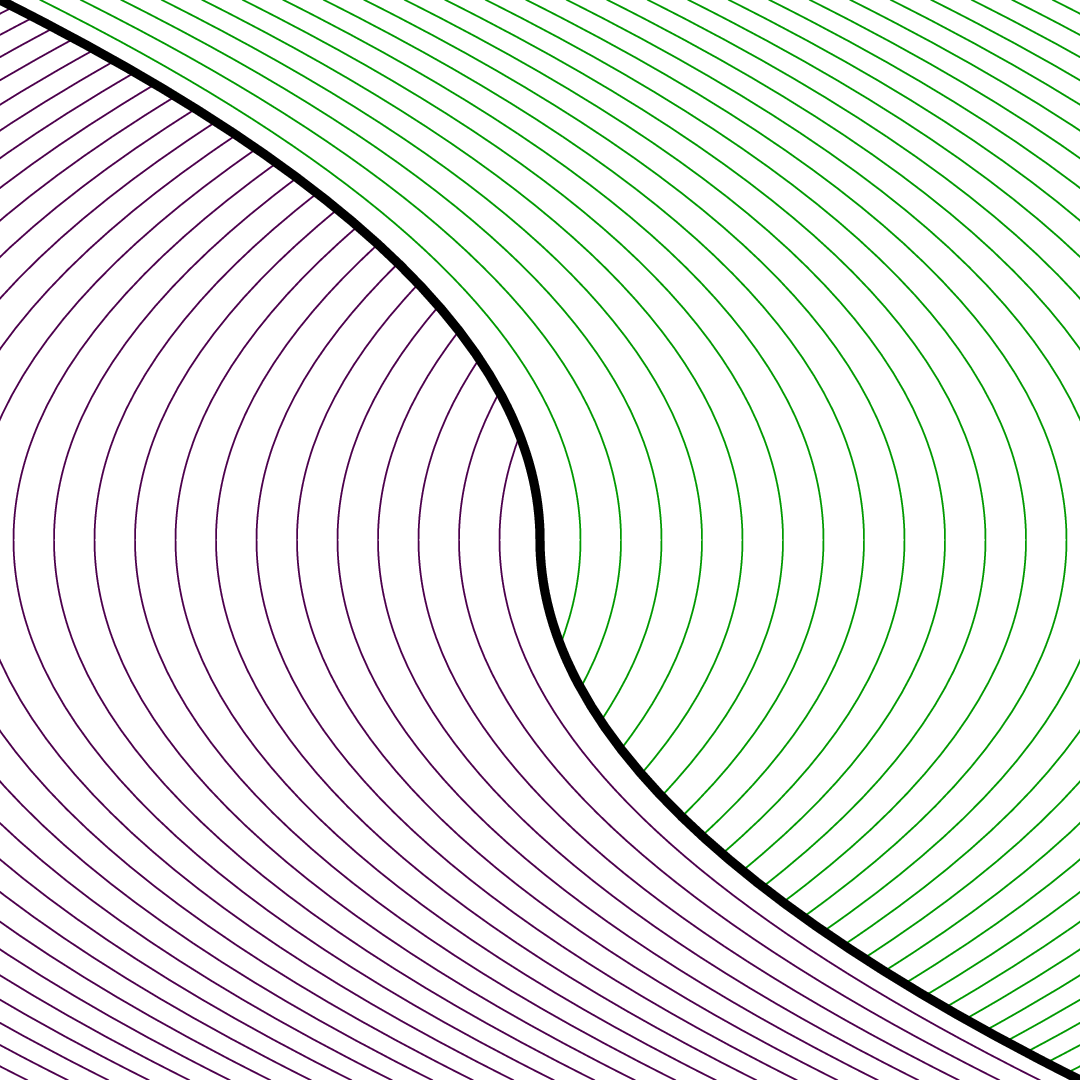
\includegraphics{figures/optimalswitching.png}}
\end{center}
\vfill
\clearpage

\pdfbookmark[0]{Contents}{toc}
\tableofcontents

\chapter{Part 1 — Hamiltonian and Lagrangian mechanics}

\section{Introduction}

Newton made the famous discovery that the motion of
physical bodies can be described by a second-order
differential equation

\begin{align*}
\mathbf{F} = m \mathbf{a},
\end{align*}

\noindent where $\mathbf{a}$ is the acceleration (the second
derivative of the position of the body), $m$ is the
mass, and $\mathbf{F}$ is the force, which has to be
specified in order for the motion to be determined
(for example, Newton's law of gravity gives a formula
for the force $\mathbf{F}$ arising out of the
gravitational influence of celestial bodies). The
quantities $\mathbf{F}$ and $\mathbf{a}$ are vectors,
but in simple problems where the motion is along only
one axis can be taken as scalars.

In the 18th and 19th centuries it was realized that
Newton's equations can be reformulated in two
surprising ways. The new formulations, known as
\emph{Lagrangian} and \emph{Hamiltonian} mechanics, make it
easier to analyze the behavior of certain mechanical
systems, and also highlight important theoretical
aspects of the behavior of such systems which are not
immediately apparent from the original Newtonian
formulation. They also gave rise to an entirely new
and highly useful branch of mathematics called the
\emph{calculus of variations} --- a kind of ``calculus on
steroids'' (see Section \ref{sec:variational-calculus}).

Our goal in this chapter is to give an introduction
to this deep and beautiful part of the theory of
differential equations. For simplicity, we restrict
the discussion mostly to systems with one degree of
freedom, and comment only briefly on
higher-dimensional generalizations.

\section{Hamiltonian systems}

Recall that the general form of a planar differential
equation (i.e., a system of two first-order ODEs) is

\begin{equation*} \tag{1}\label{eq:genericsystem}
\begin{split}
\dot{p} &= F(p,q,t), \\
\dot{q} &= G(p,q,t),
\end{split}
\end{equation*}

\noindent where, in keeping with a tradition in the theory of
ODEs, $\dot{f}$ denotes the derivative of a quantity
$f$ with respect to the time variable $t$. The system
is called a \emph{Hamiltonian system} if there is a
function

\[
H=H(p,q,t)
\]

\noindent (called the \emph{Hamiltonian} associated with the system)
such that the functions $F$ and $G$ satisfy

\[
F(p,q,t) = -\frac{\partial H}{\partial q}, \quad G(p,q,t) = \frac{\partial H}{\partial p}.
\]

\noindent In this case the system has the form

\begin{equation*} \tag{2}\label{eq:hamiltoniansystem}
\begin{split}
\dot{p} &= -\frac{\partial H}{\partial q}, \\
\dot{q} &= \ \ \frac{\partial H}{\partial p}.
\end{split}
\end{equation*}

\noindent The variable $p$ is sometimes called a \emph{generalized
coordinate}, and the variable $q$ is called the
\emph{generalized momentum} associated to $p$.

When can we say that a given system
\eqref{eq:genericsystem} is Hamiltonian? Assuming that $F$
and $G$ are continuously differentiable, it is not
difficult to see that a necessary condition is that

\begin{equation*} \tag{3}\label{eq:hamiltonian-sufficient}
\begin{split}
\frac{\partial F}{\partial p} = -\frac{\partial G}{\partial q},
\end{split}
\end{equation*}

\noindent (or
$\frac{\partial F}{\partial p} +\frac{\partial
G}{\partial q}=0$)
since both sides of the equation are equal to
$-\frac{\partial^2 H}{\partial p \partial q}$.
Equivalently, this condition can be written as

\[
\operatorname{div} \mathbf{V} = 0,
\]

\noindent where $\mathbf{V}$ denotes the planar vector field
$\mathbf{V}= (F,G)$ (we interpret the first
coordinate of $\mathbf{V}$ as the ``$p$-coordinate''
and the second coordinate as the ``$q$-coordinate''),
and $\operatorname{div} \mathbf{V}$ denotes the
divergence of $\mathbf{V}$. In physics, a vector
field with this property is called \emph{divergence-free}
or \emph{solenoidal}. Yet another way to write
\eqref{eq:hamiltonian-sufficient} is

\begin{align*}
\operatorname{curl} \mathbf{W} = 0,
\end{align*}

\noindent where $\mathbf{W}$ is the vector field
$\mathbf{W}=(G,-F)$, and $\operatorname{curl}$ is the
(2-dimensional version of the) curl operator, defined
by
$\operatorname{curl}(A,B) = \frac{\partial
A}{\partial q}-\frac{\partial B}{\partial p}$.
A vector field with this property is called
\emph{curl-free} or \emph{irrotational}.

\begin{lem}
\label{lem:hamiltonian-div}
If the equation \eqref{eq:genericsystem} is defined on a
simply connected domain, the condition
\eqref{eq:hamiltonian-sufficient} is both necessary and
sufficient for the system to be Hamiltonian.
\end{lem}

\begin{proof}
This is a slight reformulation of a familiar fact
from vector calculus, that says that in a simply
connected domain, a vector field $\mathbf{W}=(A,B)$
is curl-free if and only if it is \emph{conservative}. A
conservative vector field is one for which the line
integral of the field between two points is
independent of the contour connecting them, or
equivalently, such that the line integral on any
\emph{closed} contour vanishes. Such a vector field can
always be represented as $\mathbf{W} = \nabla H$ (the
gradient of $H$) for some scalar function $H$; one
simply defines $H(p,q)$ as the line integral (which
for a conservative field is independent of the path of
integration)

\[
H(p,q) = \int_{(p_0,q_0)}^{(p,q)} \mathbf{W}\cdot \mathbf{ds} = \int_{(p_0,q_0)}^{(p,q)} A\,dp + B\,dq
\]

\noindent between some fixed but arbitrary initial point
$(p_0,q_0)$ and the point $(p,q)$. The fact that
$\mathbf{W}=\nabla H$ is immediate from the
fundamental theorem of calculus. In our case,
$\mathbf{W}=(G,-F)$ so the equation
$\mathbf{W}=\nabla H$ gives exactly the pair of
equations $F=-\frac{\partial H}{\partial q}$,
$G=\frac{\partial H}{\partial p}$, with $H$ serving
as the desired Hamiltonian.
\end{proof}

\section{The Euler-Lagrange equation}

Given a function of three variables
$L=L(\dot{q},q,t)$, the differential equation

\begin{equation*} \tag{4}\label{eq:euler-lagrange}
\begin{split}
\frac{d}{dt}\left( \frac{\partial L}{\partial \dot{q}} \right) = \frac{\partial L}{\partial q}
\end{split}
\end{equation*}

\noindent is called the \emph{Euler-Lagrange equation}. Note that
the notation here may be slightly confusing: for the
purpose of computing $L(\dot{q},q,t)$ and finding
$\frac{\partial L}{\partial \dot{q}}$, one must think
of $\dot{q}$ as an independent variable that has no
connection to $q$. But once
$\frac{\partial L}{\partial \dot{q}}$ is evaluated,
to apply the time-derivative $\frac{d}{dt}$, one
should think of $\dot{q}$ as the time-derivative of
$q$. This leads to a second-order ordinary
differential equation for the quantity $q$. The
function $L$ is called the \emph{Lagrangian}.

\section{Equivalence of the Lagrange and Hamilton formalisms}

We now wish to show that the Euler-Lagrange equation
is equivalent to the idea of a Hamiltonian system.
Start with the equation \eqref{eq:euler-lagrange}. Denote
$p=\frac{\partial L}{\partial \dot{q}}$. The
Hamiltonian will be defined by

\begin{equation*} \tag{5}\label{eq:hamilton-lagrange}
\begin{split}
H(p,q,t) = p\dot{q} - L(\dot{q}, q, t),
\end{split}
\end{equation*}

\noindent where $\dot{q}$ is again interpreted as a symbol
representing an independent variable, which is
extracted from $p, q, t$ by inverting the relation
$p=\frac{\partial L}{\partial \dot{q}}$ (i.e., this
relation defines a transformation from the system of
variables $\dot{q},q,t$ to the system $p,q,t$). Then,
using the chain rule we can compute

\begin{align*}
\frac{\partial H}{\partial p} &= \dot{q} + p \frac{\partial \dot{q}}{\partial p} - \frac{\partial L}{\partial \dot{q}} \frac{\partial \dot{q}}{\partial p} =
\dot{q} + p \frac{\partial \dot{q}}{\partial p} - p \frac{\partial \dot{q}}{\partial p} = \dot{q}, \\
\frac{\partial H}{\partial q} &= p \frac{\partial \dot{q}}{\partial q} - \frac{\partial L}{\partial \dot{q}}\frac{\partial \dot{q}}{\partial q}-\frac{\partial L}{\partial q} = -\frac{\partial L}{\partial q} =
- \frac{d}{dt} \left( \frac{\partial L}{\partial \dot{q}}\right) = -\frac{dp}{dt} = -\dot{p},
\end{align*}

\noindent which shows that we indeed get the Hamiltonian system
\eqref{eq:hamiltoniansystem}.

Going in the other direction, if we start with a
Hamiltonian system, we can construct a Lagrangian by
setting

\begin{equation*} \tag{6}\label{eq:lagrange-hamilton}
\begin{split}
L(\dot{q}, q, t) = p\dot{q} - H(p,q,t),
\end{split}
\end{equation*}

\noindent where in this definition $p=p(q,\dot{q},t)$ is
interpreted as a function of the independent variables
$q, \dot{q}, t$, defined by the implicit equation
$\dot{q} = \frac{\partial H}{\partial p}$. Again
computing using the chain rule and the Hamiltonian
equations \eqref{eq:hamiltoniansystem}, we now have that

\begin{align*}
\frac{\partial L}{\partial \dot{q}} &= p + \dot{q} \frac{\partial p}{\partial \dot{q}} - \frac{\partial H}{\partial p} \frac{\partial p}{\partial \dot{q}} = p, \\
\frac{\partial L}{\partial q} &= \dot{q}\frac{\partial p}{\partial q}-\frac{\partial H}{\partial p}\frac{\partial p}{\partial q}-\frac{\partial H}{\partial q}=-\frac{\partial H}{\partial q}=\dot{p} = \frac{d}{dt}
\left( \frac{\partial L}{\partial \dot{q}} \right),
\end{align*}

\noindent so we have recovered the Euler-Lagrange equation
\eqref{eq:euler-lagrange}.

\begin{xexercise}[Legendre transform]
The connection between the Hamiltonian and Lagrangian
is that each is obtained from the other via a
transformation called the \emph{Legendre transform}. Here
is a simplified version of the definition of this
transform: given a strictly convex smooth function
$f(x)$ defined on some interval $[x_0,x_1]$ (i.e.,
$f''>0$), its Legendre transform is a function $g(p)$
defined on the interval $[p_0,p_1]$, where
$p_i=f'(x_i)$. To compute $g(p)$, we first find the
point $x$ such that $p=f'(x)$, and then set

\begin{align*}
g(p) = px - f(x).
\end{align*}

\begin{enumerate}[label=\arabic*.]
\item Prove that $g$ is also strictly convex.

\item Prove that the Legendre transform is its own inverse:
i.e., $f(x)$ is the Legendre transform of $g(p)$.

\item Compute the Legendre transforms of the following
functions: (i) $f(x)=x^{\alpha}, \alpha>1$; (ii)
$f(x)=e^x$; (iii) $f(x)=\cosh x$.
\end{enumerate}

\end{xexercise}

\section{Lagrangian formulation of Newtonian mechanics}

Assume a particle of mass $m$ is constrained to move
in one dimension under the influence of a force
$F=F(q,t)$, where $q$ is the position coordinate. The
equation of motion is

\begin{equation*} \tag{7}\label{eq:newtonmotion}
\begin{split}
\ddot{q} = \frac{F}{m} = -\frac{\partial U}{\partial q},
\end{split}
\end{equation*}

\noindent where $U=U(q,t)$ is the potential energy per unit
mass associated with the force $F$ at time $t$,
defined by $U(q)=-\frac{1}{m}\int_{q_0}^ q F(u)\,du$.
Define a Lagrangian $L=L(\dot{q},q,t)$ by

\[
L(\dot{q},q,t) = \tfrac12 \dot{q}^2 - U(q,t)
\]

\noindent (the kinetic energy of the particle \emph{minus} the
potential energy, divided by its mass). Now let us
write the Euler-Lagrange equation for this Lagrangian.
The relation
$p=\frac{\partial L}{\partial q} = \dot{q}$ means
that $p$ is simply equal to the velocity of the
particle, and \eqref{eq:euler-lagrange} becomes

\[
\ddot{q} = \dot{p} = \frac{d}{dt} \left( \frac{\partial L}{\partial \dot{q}} \right) = \frac{\partial L}{\partial q} = -\frac{\partial U}{\partial q},
\]

\noindent which is the same as \eqref{eq:newtonmotion}. The
strange-looking Lagrangian formalism has reproduced
Newton's equation of motion! Also note that the
Hamiltonian associated with the system, related to the
Lagrangian by equations \eqref{eq:hamilton-lagrange} and
\eqref{eq:lagrange-hamilton}, is

\begin{align*}
H = p \dot{q} - L = \dot{q}^2 - \left( \tfrac12 \dot{q}^2 - U(q,t) \right)
= \tfrac12 \dot{q}^2 + U(q,t),
\end{align*}

\noindent i.e., the Hamiltonian is the kinetic energy \emph{plus}
the potential energy, or the total energy of the
particle, divided by the mass.

Let us now see whether this phenomenon can be
generalized. Assume that the particle is now moving in
\emph{three} dimensions, so its position $\mathbf{x}(t)$
as a function of time is a vector, which varies under
the influence of an external force field, which we
take to be conservative. However, since we prefer to
keep working with planar ODEs for the time being,
assume that the motion of the particle is nonetheless
constrained to lie on some one-dimensional curve
$\Gamma=\Gamma_t$ (which could itself be moving in
space, so depends on $t$). For example, the physical
interpretation can be of a bead sliding without
friction along a curved wire, which may be moving in
space. In this case, the equation of motion can be
written in the form

\begin{equation*} \tag{8}\label{eq:curve-forces}
\begin{split}
\ddot{\mathbf{x}} - \frac{1}{m}\mathbf{F} = \ddot{\mathbf{x}} + \nabla U = \frac{1}{m} \mathbf{G}(\mathbf{x},t),
\end{split}
\end{equation*}

\noindent where $\mathbf{F}(\mathbf{x},t)$ denotes the external
force field, associated with the potential energy
$U(\mathbf{x},t)$, and where a second force function
$\mathbf{G}(\mathbf{x},t)$ is a \emph{constraint force}
acting in a direction normal to the curve $\Gamma_t$.
The role of the constraint force is to make sure that
the particle's trajectory remains constrained to the
curve.

Now, since the particle is constrained to a curve, we
should be able to describe its position at any instant
using a single real number. That means introducing a
new (scalar) quantity $q$, such that $\mathbf{x}$ can
be described in terms of a functional relation with
$q$:

\begin{align*}
\mathbf{x} = \mathbf{x}(q,t).
\end{align*}

\noindent The idea is that $q$ is a parameter measuring
position along the curve (in a way that may depend on
$t$) in some way. For example, $q$ may measure arc
length along the curve as measured from some known
reference point $\mathbf{x_0}(t)$ on the curve. The
details of the definition of $q$ depend on the
specific problem (there are many possible choices of
$q$ for a given situation) and are not important for
the present analysis.

Let us now show that the equation of motion can be
represented using the Lagrangian formalism as applied
to the new coordinate $q$. Begin by observing that we
have the relation

\begin{align*}
\mathbf{G}\cdot \frac{\partial \mathbf{x}}{\partial q} = 0,
\end{align*}

\noindent since $\mathbf{G}$ acts normally to the curve and
$\frac{\partial \mathbf{x}}{\partial q}$ is
tangential to it. Then taking the scalar product of
both sides of \eqref{eq:curve-forces} with
$\frac{\partial \mathbf{x}}{\partial q}$ gives

\begin{align*}
\ddot{\mathbf{x}} \cdot \frac{\partial \mathbf{x}}{\partial q} + (\nabla U) \cdot \frac{\partial \mathbf{x}}{\partial q} = 0,
\end{align*}

\noindent or

\begin{equation*} \tag{9}\label{eq:curveeq1}
\begin{split}
\ddot{\mathbf{x}} \cdot \frac{\partial \mathbf{x}}{\partial q} + \frac{\partial U}{\partial q} = 0,
\end{split}
\end{equation*}

\noindent where we now interpret $U=U(\mathbf{x},t)$ as a
function $U(q,t)$ of $q$ and $t$. Now define the
Lagrangian $L$ by again taking the difference of the
kinetic and potential energies, namely

\begin{align*}
L = \tfrac12 |\dot{\mathbf{x}}|^2 - U
= \tfrac12 \left| \frac{\partial \mathbf{x}}{\partial q} \dot{q} + \frac{\partial \mathbf{x}}{\partial t} \right|^2 - U,
\end{align*}

\noindent which can be interpreted as a function of $q$,
$\dot{q}$ and $t$. Note that the velocity
$\dot{\mathbf{x}}=\frac{\partial \mathbf{x}}{\partial
q} \dot{q} + \frac{\partial \mathbf{x}}{\partial t}$,
also considered as a function of $q, \dot{q}$ and $t$,
satisfies

\[
\frac{\partial \dot{\mathbf{x}}}{\partial \dot{q}} = \frac{\partial \mathbf{x}}{\partial q}.
\]

\noindent Taking partial derivatives of $L$ with respect to $q$
and $\dot{q}$, we get

\begin{equation*} \tag{10}\label{eq:curveeq2}
\begin{split}
\frac{\partial L}{\partial \dot{q}} &=
\tfrac12 \frac{\partial }{\partial \dot{q}} \left( \dot{\mathbf{x}}\cdot \dot{\mathbf{x}} \right)
=
\dot{\mathbf{x}} \cdot \frac{\partial \mathbf{x}}{\partial q}, \\
\frac{\partial L}{\partial q} &=
\tfrac12 \frac{\partial }{\partial q} \left( \dot{\mathbf{x}}\cdot \dot{\mathbf{x}} \right) - \frac{\partial U}{\partial q}
=
\dot{\mathbf{x}}\cdot \frac{\partial \dot{\mathbf{x}}}{\partial q}-\frac{\partial U}{\partial q}.
\end{split}
\end{equation*}

\noindent Also, note that

\begin{equation*} \tag{11}\label{eq:curveeq3}
\begin{split}
\frac{d}{dt}\left(\frac{\partial \mathbf{x}}{\partial q}\right) = \frac{\partial ^2 \mathbf{x}}{\partial q^2}\dot{q}
+ \frac{\partial ^2 \mathbf{x}}{\partial q\partial t} = \frac{\partial }{\partial q}
\left( \frac{\partial \mathbf{x}}{\partial q}\dot{q}+\frac{\partial \mathbf{x}}{\partial t}
\right) = \frac{\partial \mathbf{\dot{x}}}{\partial q}
\end{split}
\end{equation*}

\noindent Combining the results \eqref{eq:curveeq1},
\eqref{eq:curveeq2} and \eqref{eq:curveeq3}, we get finally
that

\begin{align*}
\frac{d}{dt}\left(\frac{\partial L}{\partial \dot{q}}\right)
&=
\ddot{\mathbf{x}} \cdot \frac{\partial \mathbf{x}}{\partial q}
+ \dot{\mathbf{x}}\cdot \frac{d}{dt}\left( \frac{\partial \mathbf{x}}{\partial q}\right)
=
\ddot{\mathbf{x}} \cdot \frac{\partial \mathbf{x}}{\partial q}
+ \dot{\mathbf{x}} \cdot \frac{\partial \dot{\mathbf{x}}}{\partial q} \\
&=
\ddot{\mathbf{x}} \cdot \frac{\partial \mathbf{x}}{\partial q}
+ \frac{\partial }{\partial q}\left(\tfrac12|\dot{\mathbf{x}}|^2\right)
= -\frac{\partial U}{\partial q}+\frac{\partial }{\partial q}(L+U) \\
&= \frac{\partial L}{\partial q}.
\end{align*}

\noindent Thus, the equation of motion becomes the
Euler-Lagrange equation for the Lagrangian $L$ when
the motion is parametrized using the scalar coordinate
$q$.

It is interesting to find also the Hamiltonian
associated with the system. Is it equal to the total
energy per unit mass? The energy per unit mass is

\begin{align*}
E = K + U,
\end{align*}

\noindent where $U$ is the potential energy and
$K = \tfrac12|\dot{x}|^2$ is the kinetic energy,
which can be written more explicitly as

\begin{align*}
K = \tfrac12 \left|\frac{\partial \mathbf{x}}{\partial q}\right|^2 \dot{q}^2 + \left(\frac{\partial \mathbf{x}}{\partial q}\cdot\frac{\partial \mathbf{x}}{\partial t}\right)
\dot{q} + \tfrac12\left|\frac{\partial \mathbf{x}}{\partial t}\right|^2,
\end{align*}

\noindent (a quadratic polynomial in $\dot{q}$). The
generalized momentum coordinate $p$ is in this case
given by

\begin{align*}
p = \frac{\partial L}{\partial \dot{q}} =
\left|\frac{\partial \mathbf{x}}{\partial q}\right|^2 \dot{q} + \frac{\partial \mathbf{x}}{\partial q}\cdot\frac{\partial \mathbf{x}}{\partial t}.
\end{align*}

\noindent Note that it is in one-to-one correspondence with
$\dot{q}$, as should happen. By
\eqref{eq:hamilton-lagrange}, we get the Hamiltonian as

\begin{align*}
H &=
\left|\frac{\partial \mathbf{x}}{\partial q}\right|^2 \dot{q}^2 + \left(\frac{\partial \mathbf{x}}{\partial q}\cdot\frac{\partial \mathbf{x}}{\partial t}\right)\dot{q} - L \\
&=
\left|\frac{\partial \mathbf{x}}{\partial q}\right|^2 \dot{q}^2 + \left(\frac{\partial \mathbf{x}}{\partial q}\cdot\frac{\partial \mathbf{x}}{\partial t}\right)\dot{q} - (K-U) \\
&= E - \left(\frac{\partial \mathbf{x}}{\partial q}\cdot\frac{\partial \mathbf{x}}{\partial t}\right)\dot{q} -
\tfrac12\left|\frac{\partial \mathbf{x}}{\partial t}\right|^2.
\end{align*}

\noindent In particular, if $\mathbf{x}$ does not have an
explicit dependence on $t$ (which corresponds to a
situation in which $\mathbf{x}=\mathbf{x}(q)$, i.e.,
the constraint curve is stationary), then
$\frac{\partial \mathbf{x}}{\partial t}=0$, and in
this case $H=E$. However, in the general case the
Hamiltonian differs from the energy of the system.

\begin{example}[The harmonic oscillator]
The one-dimensional harmonic oscillator corresponds
to the motion of a particle in a parabolic potential
well, $U(q)=\tfrac12 k q^2$, where $k>0$, or
equivalently, motion under a linear restoring force
$F(q)=-m k q$ (e.g., an oscillating weight attached
to an idealized elastic spring satisfiying Hooke's
law). In this case we have

\begin{align*}
L &= \tfrac12 \dot{q}^2 - \tfrac12 kq^2, \\
H &= \tfrac12 \dot{q}^2 + \tfrac12 kq^2, \\
p &= \frac{\partial L}{\partial \dot{q}} = \dot{q},
\end{align*}

\noindent and the equation of motion
$\frac{d}{dt}\left(\frac{\partial L}{\partial
\dot{q}}\right)=\frac{\partial L}{\partial q}$
is

\begin{align*}
\ddot{q} = -kq.
\end{align*}

\noindent Its general solution has the form

\begin{align*}
q = A\cos(\omega t) + B \sin(\omega t),
\end{align*}

\noindent where $\omega= \sqrt{k}$.
\end{example}

\begin{example}[The simple pendulum]
Next, consider the simple pendulum, which consists of
a point mass $m$ attached to the end of a rigid rod
of length $\ell$ and negligible mass, whose other end
is fixed to a point and is free to rotate in one
vertical plane. This simple mechanical system also
exhibits oscillatory behavior, but its behavior is
much richer and more complex due to the nonlinearity
of the underlying equation of motion. Let us use the
Lagrangian formalism to derive the equation of motion.
This is an example of the more generalized scenario of
motion constrained to a curve (in this case a circle).
The natural choice for the generalized coordinate $q$
is the angle $q=\theta$ between the two vectors
pointing from the fixed end of the rod in the down
direction and towards the pendulum, respectively. In
this case, we can write

\begin{align*}
\mathbf{x} &= (\ell\sin q, 0, -\ell \cos q), \\
K &= \textrm{Kinetic energy per unit mass} = \tfrac12|\dot{\mathbf{x}}|^2 = \tfrac12 \ell^2 \dot{q}^2, \\
U &= \textrm{Potential energy per unit mass} = -g\ell\cos q, \\
L &= K-U = \tfrac12 \ell^2 \dot{q}^2 + g \ell \cos q, \\
p &= \frac{\partial L}{\partial \dot{q}} = \ell^2 \dot{q}, \\
H &= E = K+U = \tfrac12 \ell^2 \dot{q}^2 - g \ell\cos q
= \frac{p^2}{2\ell^2} - g\ell\cos q.
\end{align*}

\noindent The equation of motion becomes
$\ell^2 \ddot{q}=\dot{p} = \frac{\partial L}{\partial
q}=-g\ell \sin q$,
or

\begin{align*}
\ddot{q} = -\frac{g}{\ell} \sin q.
\end{align*}

\noindent This is often written in the form

\begin{equation*} \tag{12}\label{eq:pendulumeq}
\begin{split}
\ddot{q} + \omega^2 \sin q = 0,
\end{split}
\end{equation*}

\noindent where $\omega^2 = \frac{g}{\ell}$. In Hamiltonian
form, the equations of motion will be

\begin{align*}
\dot{p}&= -g\ell \sin q, \\ \dot{q}&=\frac{p}{\ell^2}.
\end{align*}

\end{example}

\begin{example}[A rotating pendulum]
Let us complicate matters by assuming that the
pendulum is rotating around the vertical axis (the
$z$-axis, in our coordinate system) with a fixed
angular velocity $\omega$. In terms of the coordinate
$q$, which still measures the angle subtended between
the vector pointing from the origin to the particle
and the vertical, the particle's position will now be

\begin{align*}
\mathbf{x} = (\ell \sin q \cos(\omega t), \ell \sin q \sin(\omega t), -\ell\cos(\omega t)).
\end{align*}

\noindent The kinetic and potential energies per unit mass, and
from them the Lagrangian and Hamiltonian, and the
generalized momentum coordinate $p$, can now be found
to be

\begin{align*}
K &= \tfrac12|\dot{x}|^2 = \tfrac12 \ell^2(\dot{q}^2 + \omega^2 \sin^2 q), \\
U &= -g\ell \cos q, \\
L &= \tfrac12\ell^2(\dot{q}^2+\omega^2\sin^2 q)+g\ell\cos q, \\
p &= \ell^2 \dot{q}, \\
H &= \frac{p^2}{2\ell^2}-g\ell\cos q-\tfrac12 \omega^2 \ell^2 \sin^2 q.
\end{align*}

\noindent The Euler-Lagrange equation of motion is

\begin{align*}
\ddot{q} + \Omega^2 \sin q - \omega^2 \sin q \cos q = 0,
\end{align*}

\noindent where $\Omega^2 = \frac{g}{\ell}$. The system in
Hamiltonian form is

\begin{align*}
\dot{p} &= -g\ell \sin q + \omega^2 \ell^2 \sin q \cos q, \\
\dot{q} &= \frac{p}{\ell^2}.
\end{align*}

\end{example}

\section{An autonomous Hamiltonian is conserved}

In the last example above, it is important to note
that although the system in its original form depends
on time due to the motion of the constraint curve, the
Hamiltonian, Lagrangian and the associated equations
are \emph{autonomous}, i.e., do not depend on time. This is
an illustration of the type of simplification that can
be achieved using the Lagrangian and Hamiltonian
formulations. Furthermore, the fact that the
Hamiltonian is autonomous has an important
consequence, given by the following lemma.

\begin{lem}
\label{lem:hamiltonian-conserved}
If the Hamiltonian is autonomous, then $H$ is an
integral (i.e., an invariant or conserved quantity) of
Hamilton's equations.
\end{lem}

\begin{proof}
The assumption means that
$\frac{\partial H}{\partial t} = 0$. By the chain
rule, it follows that

\begin{align*}
\frac{dH}{dt} &= \frac{\partial H}{\partial p} \dot{p}+\frac{\partial H}{\partial q} \dot{q} + \frac{\partial H}{\partial t} \\
&= \frac{\partial H}{\partial p}\left(-\frac{\partial H}{\partial q}\right)+\frac{\partial H}{\partial q}\left(\frac{\partial H}{\partial p}\right)+\frac{\partial H}{\partial t}
= \frac{\partial H}{\partial t} = 0.
\end{align*}

\end{proof}

\noindent In the first two examples of the harmonic oscillator
and the simple pendulum, the Hamiltonian was equal to
the system's energy, so \texorpdfstring{\hyperref[lem:hamiltonian-conserved]{Lemma~\ref*{lem:hamiltonian-conserved}}}{Lemma} corresponds to the
conservation of energy. In the example of the rotating
pendulum, the Hamiltonian is \emph{not} equal to the energy
of the system, yet it is conserved. Can you think of a
physical meaning to assign to this conserved quantity?

\section{Systems with many degrees of freedom}

In the above discussion, we focused on a system with
only one degree of freedom. In this case the equations
of motion consisted of a single second order
differential equation (the Euler-Lagrange equation),
or in the equivalent Hamiltonian form, a planar system
of first-order equations. We can describe the behavior
of systems having more degrees of freedom, involving
for example many particles or an unconstrained
particle moving in three dimensions, using a
multivariate form of the Euler-Lagrange and Hamilton
equations. We describe these more general formulations
of the laws of mechanics briefly, although we will not
develop this general theory here.

Let the system be described by $n$ generalized
coordinates $q_1, \ldots, q_n$. The Lagrangian will
be a function of the coordinates and their time
derivatives (generalized velocities):

\begin{align*}
L = L(q_1,\ldots,q_n,\dot{q}_1,\ldots,\dot{q}_n, t)
\end{align*}

\noindent As before, the Lagrangian will be defined as the
kinetic energy minus the potential energy of the
system. The equations of motion will be given as a
system of Euler-Lagrange second-order equations, one
for each coordinate:

\begin{align*}
\frac{d}{dt}\left( \frac{\partial L}{\partial \dot{q}_j} \right) = \frac{\partial L}{\partial q_j} \ \ \quad (j=1,\ldots,n).
\end{align*}

\noindent To write the Hamiltonian formulation of the system,
first we define generalized momentum coordinates
$p_1,\ldots,p_n$. They are given analogously to the
one-dimensional case by

\begin{align*}
p_j = \frac{\partial L}{\partial \dot{q}_j} \ \ \quad (j=1,\ldots,n).
\end{align*}

\noindent The Hamiltonian system is written as a system of $2n$
first-order ODEs:

\begin{align*}
\begin{array}{rl} \displaystyle
\dot{p}_j &= \displaystyle-\frac{\partial H}{\partial q_j}, \\
\displaystyle \dot{q}_j &= \displaystyle \ \ \frac{\partial H}{\partial p_j},
\end{array} \qquad (j=1,\ldots,n),
\end{align*}

\noindent where $H=H(p_1,\ldots,p_n,q_1,\ldots,q_n, t)$ is the
Hamiltonian, which (like the Lagrangian) is still a
scalar function. This is sometimes written as the pair
of vector equations

\begin{align*}
\dot{\mathbf{p}} &= -\frac{\partial H}{\partial \mathbf{q}}, \\
\dot{\mathbf{q}} &= \ \ \frac{\partial H}{\partial \mathbf{p}},
\end{align*}

\noindent where we denote $\mathbf{p}=(p_1,\ldots,p_n)$,
$\mathbf{q}=(q_1,\ldots,q_n)$.

As in the case of one-dimensional systems, it can be
shown that (under some mild assumptions) the
Hamiltonian and Lagrangian formulations are
equivalent, and that they correctly describe the laws
of motion for a Newtonian mechanical system if the
Lagrangian is defined as the kinetic energy minus the
potential energy. The relationship between the
Lagrangian and Hamiltonian is given by

\begin{align*}
H = \sum_{j=1}^n \dot{q}_j p_j - L.
\end{align*}

\begin{example}[A pendulum with a cart]
An important example that we will discuss later from
the point of view of control theory is that of a
simple pendulum whose point of support is allowed to
slide without friction along a horizontal axis (e.g.,
you can imagine the pendulum hanging on a cart with
wheels rolling on a track of some sort). We assume the
sliding support has mass $M$. This system has two
degrees of freedom: the angle $q_1 = \theta$ between
the pendulum and the vertical line extending down from
the point of support, and the distance $q_2 = s$
(measured in the positive $x$ direction) between the
point of support and some fixed origin. To derive the
equations of motion, we write the kinetic and
potential energies:

\begin{align*}
K &= \tfrac12 M \dot{s}^2 + \tfrac12 m \left[ \left(\dot{s}+\ell \dot{\theta} \cos \theta \right)^2 + \left(\ell \dot{\theta} \sin \theta \right)^2 \right], \\
U &= -mg \ell \cos \theta.
\end{align*}

\noindent The Lagrangian $L=K-U$ is then given by

\begin{align*}
L &=
\tfrac12 M \dot{s}^2 + \tfrac12 m \left[ \left(\dot{s}+\ell \dot{\theta} \cos \theta \right)^2 + \left(\ell \dot{\theta} \sin \theta \right)^2 \right] + mg \ell \cos \theta \\
&= \tfrac12(M+m)\dot{s}^2 + m\ell \dot{s} \dot{\theta} \cos \theta + \tfrac12 m \ell^2 \dot{\theta}^2 + mg\ell \cos\theta.
\end{align*}

\noindent Therefore the equations of motion
$\frac{d}{dt}\left(\frac{\partial L}{\partial
\dot{s}}\right)=\frac{\partial L}{\partial s}$,
$\frac{d}{dt}\left(\frac{\partial L}{\partial
\dot{\theta}}\right)=\frac{\partial L}{\partial
\theta}$
become

\begin{align*}
\frac{d}{dt}\left[ (M+m)\dot{s} + m\ell\dot{\theta}\cos \theta \right] &= 0, \\
\frac{d}{dt}\left[m(\ell \dot{s}  \cos\theta + \ell^2 \dot{\theta})\right] &= -m(\ell\dot{s} \dot{\theta} + g\ell)\sin \theta,
\end{align*}

\noindent or, written more explicitly,

\begin{align*}
(M+m)\ddot{s} + m\ell \ddot{\theta} \cos \theta -m\ell \dot{\theta}^2 \sin\theta &= 0, \\
\ddot{\theta} + \frac{1}{\ell}\ddot{x} \cos\theta + \frac{g}{\ell}  \sin\theta &= 0.
\end{align*}

\end{example}

\begin{example}[Double pendulum]
The double pendulum consists of a mass $M$ hanging at
the end of a rigid rod of negligible mass whose other
end is attached to a fixed point of support, and
another equal (for simplicity) mass hanging from
another rigid rod, also of negligible mass attached to
the free end of the first rod. Denote by $L_1$ and
$L_2$ the respective lengths of the two rods. If we
denote by $\theta_1, \theta_2$ the angles each of the
rods forms with the vertical, a short computation
gives the Lagrangian of the system:

\begin{equation*} \tag{13}\label{eq:lagrangian-doublepend}
\begin{split}
L &= K-U =
L_1 \dot{\theta}_1^2 + \tfrac12 L_2 \dot{\theta}_2^2 + L_1 L_2 \cos(\theta_1-\theta_2) \\
& \qquad\qquad \qquad +2gL_1 \cos \theta_1 + gL_2 \cos \theta_2.
\end{split}
\end{equation*}

\noindent It follows that the generalized momenta are given by

\begin{align*}
p_1 &= \frac{\partial L}{\partial \dot{\theta}_1} = \tfrac12 L_1^2 \dot{\theta}_1 - 2 L_1 L_2 \sin(\theta_1-\theta_2), \\
p_2 &= \frac{\partial L}{\partial \dot{\theta}_2} = \tfrac12 L_2^2 \dot{\theta}_2 + 2 L_1 L_2 \sin(\theta_1 - \theta_2),
\end{align*}

\noindent and from this we get the equations of motion for the
system:

\begin{align*}
\tfrac12 L_1^2 \ddot{\theta}_1 - 2 L_1 L_2 \cos(\theta_1-\theta_2)\dot{\theta}_1 &=
- L_1 L_2 \sin(\theta_1-\theta_2) + g L_1 \sin\theta_1, \\
\tfrac12 L_2^2 \ddot{\theta}_2 - 2 L_1 L_2 \cos(\theta_1-\theta_2)\dot{\theta}_2 &=
L_1 L_2 \sin(\theta_1-\theta_2) + gL_2 \sin\theta_2.
\end{align*}

\noindent This system of two nonlinear coupled second-order
ODEs is in practice impossible to solve analytically,
and for certain values of the energy is known to
exhibit chaotic behavior which is difficult to
understand in any reasonable sense; see Figure 1.
(Nonetheless, later in the course we will learn about
some interesting things that can still be said about
such systems.)

\begin{center}

\includegraphics[width=0.60\linewidth]{figures/doublependulum-flips.png}\\[0.6em]
{\small Figure 1: A color-coded map of the time required for
the double pendulum to flip over as a function of its
initial conditions reveals a chaotic structure.
(Source: Wikipedia)}
\end{center}

\end{example}

\begin{xexercise}[The Lorentz force]
From the study of electricity and magnetism, it is
known that the motion of a charged particle with mass
$m$ and electric charge $q$ is described by the
equation $\mathbf{F}=m \ddot{\mathbf{x}}$, where
$\mathbf{x}$ is the (vector) position of the particle
and $\mathbf{F}$ is the \emph{Lorentz force}, given by

\[
\mathbf{F} = q\left(\mathbf{E} + \dot{\mathbf{x}}\times \mathbf{B}\right).
\]

\noindent The vector field $\mathbf{E}=\mathbf{E}(x,y,z,t)$ is
the \emph{electric field}, and the vector field
$\mathbf{B}=\mathbf{B}(x,y,z,t)$ is the \emph{magnetic
field}. Using Maxwell's equations one can show that
there exist functions $\phi=\phi(x,y,z,t)$ and
$\mathbf{A}=\mathbf{A}(x,y,z,t)$ such that

\begin{align*}
\mathbf{E} &= - \nabla \phi - \frac{\partial \mathbf{A}}{\partial t}, \\
\mathbf{B} &= \operatorname{curl} \mathbf{A}.
\end{align*}

\noindent The (scalar) function $\phi$ is called the \emph{electric
potential}, and the vector $\mathbf{A}$ is called the
\emph{magnetic potential}, or \emph{vector potential}. Note that
$\mathbf{E}$ behaves exactly like a conventional
force field, causing the particle an acceleration in
the direction of $\mathbf{E}$ that is equal to the
field magnitude multiplied by the (constant) scalar
$q/m$, whereas the influence of the magnetic field
$\mathbf{B}$ is of a more exotic nature, causing an
acceleration that depends on the particle's \emph{velocity}
in a direction perpendicular to its direction of
motion.

Show that motion under the Lorentz force is
equivalent to the Euler-Lagrange equation
$\frac{d}{dt}\left(\frac{\partial L}{\partial
\dot{\mathbf{x}}}\right)=\frac{\partial L}{\partial
\mathbf{x}}$,
where the Lagrangian is given by

\[
L(\dot{\mathbf{x}},\mathbf{x},t) = \tfrac12 m |\dot{\mathbf{x}}|^2 - q \phi(\mathbf{x},t) +q \mathbf{A}(\mathbf{x},t)\cdot \dot{\mathbf{x}}.
\]

\end{xexercise}

\section{Rest points in autonomous Hamiltonian systems}

Assume that the Hamiltonian is autonomous. The rest
points of the system correspond to the stationary
points of the Hamiltonian, i.e., points for which

\begin{align*}
\frac{\partial H}{\partial p} = 0, \quad \frac{\partial H}{\partial q} = 0.
\end{align*}

\noindent Let $(p_0,q_0)$ be a rest point of the system. We can
analyze the stability properties of the rest point by
linearizing. Setting

\begin{align*}
x = p-p_0, \quad y=q-q_0,
\end{align*}

\noindent the behavior of the system near $(p_0,q_0)$ can be
described as

\begin{align*}
\dot{x} &= -bx-cy + O(x^2+y^2), \\ \dot{y}&= \ \ ax+by + O(x^2+y^2),
\end{align*}

\noindent where

\begin{align*}
a = \frac{\partial^2 H}{\partial p^2} \Big|_{(p_0,q_0)},\quad
b = \frac{\partial^2 H}{\partial p \partial q} \Big|_{(p_0,q_0)}, \quad
c = \frac{\partial^2 H}{\partial q^2} \Big|_{(p_0,q_0)}.
\end{align*}

\noindent By the theory of stability analysis of planar ODEs,
the stability type of the rest point can now be
understood in terms of the behavior of the eigenvalues
of the matrix

\begin{align*}
\left(\begin{array}{cc} -b&-c\\a&b\end{array}\right)
\end{align*}

\noindent (the Jacobian matrix of the vector field at the rest
point). The eigenvalues are given by

\begin{align*}
\lambda^2 = b^2-ac.
\end{align*}

\noindent So we see that, when $b^2<ac,$ the eigenvalues are
pure imaginary numbers, and recall that in that case
the rest point is a center. On the other hand, when
$b^2>ac$ the eigenvalues are the two real square
roots $\pm \sqrt{b^2-ac}$. Since in that case we have
one negative and one positive eigenvalue, the
stability theory says that the rest point is a saddle
point. (We assume that the Hessian matrix of second
derivatives is non-degenerate, i.e., that
$b^2\neq ac$, so that the usual criteria for
stability apply.) Liouville's theorem, which we will
discuss in a later section, will give another, more
geometric, explanation why rest points cannot be
asymptotically stable or unstable.

\section{The principle of least action}

For times $t_0<t_1$, define the \emph{action}$A(t_0,t_1)$
of a Lagrangian system from time $t_0$ to time $t_1$
as the integral of the Lagrangian:

\begin{align*}
A(t_0,t_1)=\textrm{action} = \int_{t_0}^{t_1} L(\dot{q}(t),q(t),t)\,dt.
\end{align*}

\noindent The action is a function of an arbitrary curve $q(t)$.
The \emph{principle of least action} is the statement that
if the system was in coordinate $q_0$ at time $t_0$
and in coordinate $q_1$ at time $t_1$, then its
trajectory between time $t_0$ and time $t_1$ is that
curve which minimizes the action $A(t_0,t_1)$,
subject to the constraints $q(t_0)=q_0, q(t_1)=q_1$.
This is a surprising statement, which we will see is
\emph{almost} equivalent to the Euler-Lagrange equation ---
only almost, since, to get the equivalence, we will
need to first modify the principle slightly to get the
more precise version known as the \emph{principle of
stationary action}.

The principle of least action can be thought of as a
strange, \emph{non-causal} interpretation of the laws of
mechanics. We are used to thinking of the laws of
nature as manifesting themselves through interactions
that are local in space and time: a particle's
position $\mathbf{x}+d\mathbf{x}$ and velocity
$\mathbf{v}+d\mathbf{v}$ at time $t+dt$, are related
to its position $\mathbf{x}$ and velocity $\mathbf{v}$
at time $t$, as well as to external forces acting on
the particle, which are also determined by ``local''
events in the vicinity of $\mathbf{x}$ at time $t$.
This way of thinking can be thought of as the \emph{causal}
interpretation, in which every effect produced at a
given point in space and time is immediately preceded
by, and can be directly attributable to, another event
causing the effect. Mathematically, this means the
laws of nature can be written as (ordinary or partial)
differential equations.

On the other hand, the principle of least action (and
other similar principles that appear in physics,
including in more fundamental areas of physics such as
quantum mechanics, that we know represent a more
correct view of our physical reality) can be thought
of as saying that, in order to bring a physical system
from state $A$ to state $B$ over a given period of
time, Nature somehow tries all possible ways of doing
it, and selects the one that minimizes the action. The
entire trajectory appears to be chosen ``all at
once,'' so that each part of it seems to depend on
other parts which are far away in space and time. This
rather unintuitive interpretation is nonetheless
mathematically correct, and even at the physical level
it has been suggested that there is some truth to it
(the arguments for why this is so involve deep ideas
from quantum mechanics that are beyond the scope of
this course).

\section{The calculus of variations}
\label{sec:variational-calculus}

Let us consider the problem of minimizing the action
in slightly greater generality. In many areas of
mathematics we encounter expressions of the form

\begin{equation*} \tag{14}\label{eq:functional}
\begin{split}
\Phi(q) = \int_{t_0}^{t_1} L(\dot{q}(t),q(t),t)\,dt
\end{split}
\end{equation*}

\noindent which take a (sufficiently smooth) function $q(t)$
defined on an interval $[t_0,t_1]$ and return a real
number. The form of the integrand $L(\dot{q},q,t)$
depends on the problem, and may have nothing to do
with Lagrangian mechanics (indeed, in many problems
with a geometric flavor, $t$ represents a space
variable instead of a time variable, and is therefore
often denoted by $x$; in this case, we write $q'$
instead of $\dot{q}$ for the derivative of $q$).
Usually the function $q$ is assumed to take specific
values at the ends of the interval, i.e., $q(t_0)=q_0$
and $q(t_1)=q_1$.

Such a mapping $q\mapsto \Phi(q)$ is called a
\emph{functional} --- note that a functional is just like
an ordinary function from calculus, except that it
takes as its argument an entire function instead of
only one or several real-valued arguments (that is why
we call such functions \emph{functionals}, to avoid an
obvious source of confusion). In many cases it is
desirable to find which function $q$ results in the
least and/or the greatest value $\Phi(q)$. Such a
minimization or maximization problem is known as a
\emph{variational problem} (the reason for the name is
explained below), and the area of mathematics that
deals with such problems is called the \emph{variational
calculus}, or \emph{calculus of variations}. In more
advanced variational problems the form of the
functional \eqref{eq:functional} can be more general and
depend for example on a vector-valued function
$\mathbf{q}(t)$, or on higher-order derivatives of
$q$, or on a function $q(x_1,\ldots,x_k)$ of several
variables

Here are some examples of variational problems.

\begin{enumerate}[label=\arabic*.]
\item What is the shortest curve in the plane connecting
two points? We all know it is a straight line, but how
can we prove it? (And how do we find the answer to the
same question on some complicated surface?)

\item What is the curve of given length in the plane
bounding the largest area? (It is a circle --- this
fact, which is not trivial to prove, is known as the
\emph{isoperimetric inequality}.)

\item What is the curve connecting a point $\mathbf{A}$ in
the plane with another lower point $\mathbf{B}$ such
that a ball rolling downhill without friction along
the curve from $\mathbf{A}$ to $\mathbf{B}$ under the
influence of gravity will reach $\mathbf{B}$ in the
minimal possible time? This problem is known as the
\emph{brachistochrone problem}, and stimulated the
development of the calculus of variations in the 18th
century.

\item What is the curve in the phase space of a Lagrangian
system that minimizes the action?
\end{enumerate}

\noindent The basic idea involved in solving variational
problems is as follows: if $q$ is an extremum
(minimum or maximum) point of the functional $\Phi$,
then it is also a \emph{local extremum}. That means that
for any (sufficiently smooth) function
$h:[t_0,t_1]\to \R$ satisfying $h(t_0)=h(t_1)=0$, the
function

\[
\phi_{q,h}(s) = \Phi(q+s h)=\int_{t_0}^{t_1} L(\dot{q}(t)+sh'(t),q(t)+sh(t),t)\,dt
\]

\noindent (an ordinary function of a single real variable $s$)
has a local extremum at $s=0$. From ordinary
calculus, we know that the derivative of $\phi_{q,h}$
at $0$ must be $0$:

\[
\phi_{q,h}'(0) = 0.
\]

\noindent To evaluate this derivative, differentiate under the
integral sign and integrate by parts, to get

\begin{align*}
\phi_{q,h}'(0)
&=
\int_{t_0}^{t_1} \frac{d}{ds} \Big|_{s=0}  L(\dot{q}(t)+sh'(t),q(t)+sh(t),t)\,dt
\\
&= \int_{t_0}^{t_1} \left(\frac{\partial L}{\partial \dot{q}} h'(t) + \frac{\partial L}{\partial q} h(t) \right)\,dt \\
&=
\int_{t_0}^{t_1} \left(-\frac{d}{dt}\left(\frac{\partial L}{\partial \dot{q}}\right) + \frac{\partial L}{\partial q} \right)h(t)\,dt
+ \frac{\partial L}{\partial \dot{q}} h(t)\Big|_{t=t_0}^{t=t_1} \\
&= \int_{t_0}^{t_1} \left(-\frac{d}{dt}\left(\frac{\partial L}{\partial \dot{q}}\right) + \frac{\partial L}{\partial q} \right)h(t)\,dt
\end{align*}

\noindent This brings us to an important definition. We denote

\begin{equation*} \tag{15}\label{eq:first-variation}
\begin{split}
\delta\Phi_q(h) = \int_{t_0}^{t_1} \left(-\frac{d}{dt}\left(\frac{\partial L}{\partial \dot{q}}\right) + \frac{\partial L}{\partial q} \right)h(t)\,dt,
\end{split}
\end{equation*}

\noindent and call this quantity the \emph{variation of the
functional}$\Phi$ at $q$, evaluated at $h$ (also
sometimes called the \emph{first variation of $\Phi$},
since there is also a second variation, third
variation etc., which we will not discuss; this is
where the name \emph{calculus of variations} comes from).
It is analogous to a directional derivative
$\frac{\partial f}{\partial \mathbf{u}} = \nabla f
\cdot \mathbf{u}$
of a function of several variables in calculus, in
that it measures the instantaneous rate of change of
$\Phi$ if we start from the ``point'' $q$ and head
off in a ``direction'' corresponding to the small
perturbation $s\cdot h$. We say that the function $q$
is a \emph{stationary point} of $\Phi$ if
$\delta\Phi_q(h) = 0$ for any (sufficiently smooth)
function $h$ satisfying $h(t_0)=h(t_1)=0$. With the
computation above, we have proved:

\begin{lem}
If $q$ is an extremum (minimum or maximum) of the
functional $\Phi$, then it is a stationary point.
\end{lem}

\noindent Finally, note that the formula for the variation
$\delta \Phi_q(h)$ involves a quantity that is
suspiciously reminiscent of the Euler-Langrange
equation. Indeed, we can now easily prove:

\begin{thm}
The function $q$ is a stationary point of $\Phi$ if
and only if it satisfies the Euler-Lagrange equation

\begin{align*}
\frac{d}{dt}\left( \frac{\partial L}{\partial \dot{q}} \right) = \frac{\partial L}{\partial q}.
\end{align*}

\end{thm}

\begin{proof}
It is easy to see that the integral on the right-hand
side of \eqref{eq:first-variation} is $0$\emph{for every}$h$
satisfying $h(t_0)=h(t_1)=0$ if and only if the
quantity in parentheses in the integrand vanishes for
all $t$.
\end{proof}

\noindent Reformulating this result in the language of
Lagrangian systems gives the correct version of the
principle of least action.

\begin{thm}[Principle of stationary action]
Given a mechanical system defined by a Lagrangian $L$,
the trajectory of the system between two times
$t_1<t_2$ satisfying $q(t_0)=q_0$ and $q(t_1)=q_1$ is
a stationary point of the action functional

\begin{align*}
\Phi(q) = A(t_0,t_1) = \int_{t_0}^{t_1} L(\dot{q},q,t)\,dt.
\end{align*}

\end{thm}

\noindent The stationary point which solves the Euler-Lagrange
equation will usually be a minimum point for simple
systems, but in general does not have to be. There is
a method for determining whether a given stationary
point is a minimum, maximum, or saddle point, which
involves computing the \emph{second variation} of the
functional (analogous to the Hessian matrix of second
derivatives of a function of several variables), but
we will not discuss it here.

Let us see how the theory works in a few examples to
solve some interesting variational problems.

\begin{example}[Plane geodesics]
Consider the problem of determining the shortest line
between two points $(x_1,y_1)$ and $(x_2,y_2)$, where
we assume for concreteness that $x_1<x_2$ (The
shortest line between two points on a general surface
or curved space is known as a \emph{geodesic}.) As is
well-known from the arc length formula
$ds^2=dx^2+dy^2$ from calculus, the length of a curve
$y=q(x)$ is given by

\begin{align*}
\Phi = \int_{x_1}^{x_2} \,ds = \int_{x_1}^{x_2} \sqrt{1+q'(x)^2}\,dx
= \int_{x_1}^{x_2} L(q',q)\,dx,
\end{align*}

\noindent where the ``Lagrangian'' is given by

\begin{align*}
L(q',q) = \sqrt{1+q'(x)^2}.
\end{align*}

\noindent To find the minimizing curve, we write the
Euler-Lagrange equation:

\begin{align*}
\frac{d}{dx} \left(\frac{q'(x)}{\sqrt{1+q'(x)^2}}\right) = \frac{d}{dx}\left( \frac{\partial L}{\partial q'} \right) = \frac{\partial L}{\partial q} = 0.
\end{align*}

\noindent The solution is

\begin{align*}
\frac{q'(x)}{\sqrt{1+q'(x)^2}} = \textrm{const},
\end{align*}

\noindent which is equivalent to $q'(x)=\textrm{const}$, i.e.,
we have recovered the equation for a straight line
$y=ax+b$.
\end{example}

\begin{example}[Brachistochrone problem]
In this problem, we try to find the curve connecting
the points $\mathbf{A}$ and $\mathbf{B}$ in the
plane, for which a ball rolling downhill without
friction from $\mathbf{A}$ to $\mathbf{B}$, with an
initial velocity of $0$, will take the shortest time
to arrive. We choose a coordinate system such that the
$x$-axis is the \emph{vertical} axis and points downward
for positive $x$, and such that $\mathbf{A}=(0,0)$,
$\mathbf{B}=(x_b,y_b)$ with $x_b,y_b>0$. If the curve
is given by $y=q(x)$, the time is given by the
integral along the curve

\begin{align*}
T = \int_{\mathbf{A}}^{\mathbf{B}} \frac{ds}{v},
\end{align*}

\noindent where $ds$ is the arc length element and $v$ is the
velocity of the ball at each point. More explicitly,
we have $ds = \sqrt{1+q'(x)^2}\,dx$, and
$v=\sqrt{2g x}$, where $g$ is the gravitational
constant (this follows from conservation of energy,
which gives the relation $\tfrac12 m v^2 = mgx$). So,
the functional we are trying to minimize is

\begin{align*}
T = \int_0^{x_b} L(q',q,x)\,dx,
\end{align*}

\noindent where

\begin{align*}
L(q',q,x) = \frac{\sqrt{1+q'^2}}{\sqrt{2g x}}.
\end{align*}

\noindent The Euler-Lagrange equation in this case becomes

\begin{align*}
\frac{d}{dx}\left(\frac{q'(x)}{\sqrt{2 g x(1+q'(x)^2}}\right) = 0,
\end{align*}

\noindent which therefore gives

\begin{align*}
\frac{q'(x)}{\sqrt{2 g x(1+q'(x)^2)}} = \alpha,
\end{align*}

\noindent where $\alpha$ is a constant. This can be rewritten
as

\[
\frac{q'(x)^2}{1+q'(x)^2} = x/\lambda,
\]

\noindent where $\lambda=(2\alpha^2 g)^{-1}$, and then solved
by solving for $q'$ and integrating, giving the
expression

\begin{equation*} \tag{16}\label{eq:cycloidquadrature}
\begin{split}
q(x) = \int_0^x \sqrt{\frac{u}{\lambda-u}}\,du.
\end{split}
\end{equation*}

\noindent Setting $a=\lambda/2$ and using the trigonometric
substitution

\begin{align*}
u = 2a \sin^2(\theta/2) = a(1-\cos \theta),
\end{align*}

\noindent we obtain a convenient parametric representation for
the curve, namely

\begin{align*}
x(\theta) &= a(1-\cos \theta), \\
y(\theta) &= \int_0^\theta \sqrt{\frac{1-\cos\theta}{1+\cos\theta}}\,a\sin \theta\,d\theta
= a\int_0^\theta (1-\cos\theta)\,d\theta = a(\theta-\sin\theta).
\end{align*}

\noindent These are the equations for a \emph{cycloid} (or, rather,
an \emph{inverted cycloid}, as the cycloid is usually drawn
with its ``flat'' side up): as can be seen easily from
the parametric equations, it describes the trajectory
of a point on a wheel that rolls along the $y$-axis
(the parameter $\theta$ represents the angle by which
the wheel has rolled forward; see Figure 2). The
scaling constant $a$ can now be chosen to fit the
condition that $q(x_b)=y_b$, i.e., the curve must
pass through the point $\mathbf{B}$. It may also be
verified using \eqref{eq:cycloidquadrature} that the
nonparametric equation for the cycloid is

\begin{align*}
y = q(x) = a \cos^{-1}\left(\frac{a-x}{a}\right)-\sqrt{x(2a-x)}.
\end{align*}

\end{example}

\begin{xexercise}[Tautochrone problem]

\begin{enumerate}[label=\arabic*.]
\item Find a formula for the time it takes a ball rolling
down a brachistochrone curve to get to the lowest
point on the curve.

\item Show that the inverted cycloid is also a \emph{tautochrone
curve}, i.e., it has the property that a ball placed
on the curve and allowed to roll downhill and then up
repeatedly would undergo an oscillatory motion whose
period is independent of the ball's initial position
along the curve. (This fact was discovered by
Christiaan Huygens, the famous 17th century Dutch
mathematician and astronomer. Huygens, who invented
the pendulum clock, was aware that the period of a
pendulum \emph{does} depend on its amplitude of oscillation
--- a fact which limits its accuracy for timekeeping
applications --- and tried unsuccessfully to design a
more accurate modified pendulum clock based on the
tautochrone curve.)
\end{enumerate}

\end{xexercise}

\begin{center}
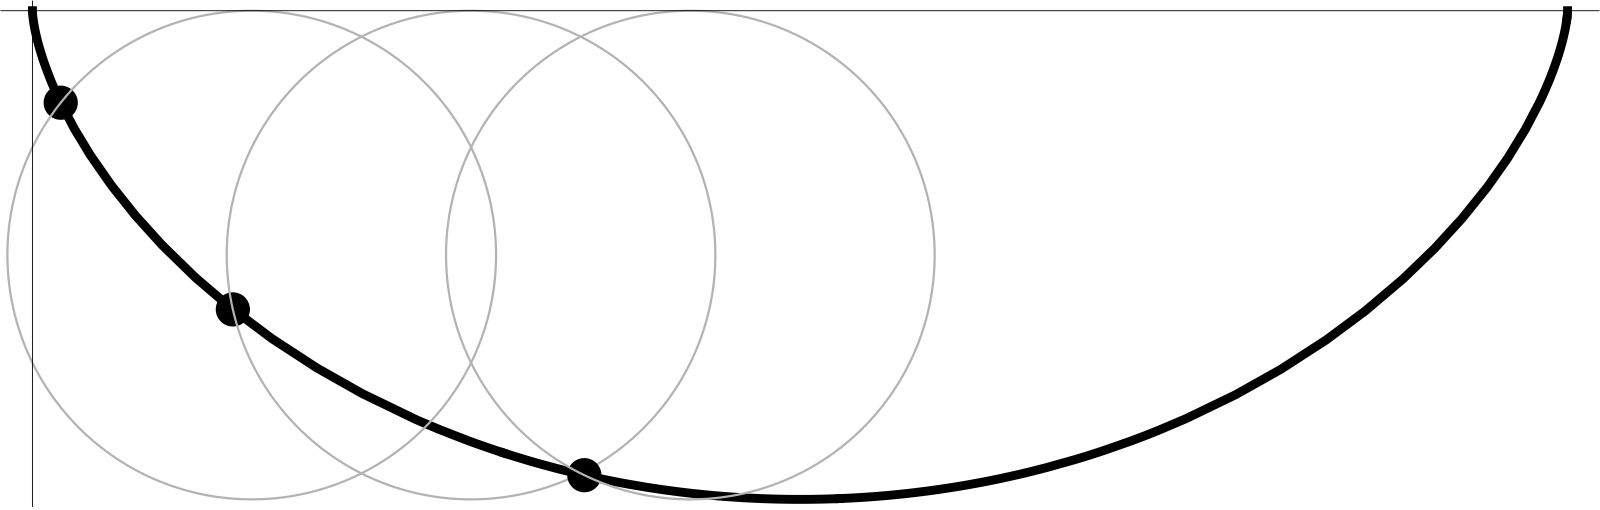
\includegraphics[width=0.90\linewidth]{figures/brachistochrone.png}\\[0.6em]
{\small Figure 2: The brachistochrone curve (cycloid) as the
trajectory of a point on the boundary of a circle
rolling on a line.}
\end{center}

\begin{example}[Geodesics in the hyperbolic plane]
The hyperbolic plane is a well-known example of a
\emph{non-Euclidean geometry}, i.e., a geometry in which
Euclid's parallel postulate fails to hold. A concrete
realization of the hyperbolic plane consists of the
set

\begin{align*}
\mathbb{H} = \{ (x,y)\in \mathbb{R}^2\,:\, y>0 \}
\end{align*}

\noindent (known as the \emph{upper half plane} in complex
analysis), together with a modified formula for the
arc length of a line segment, namely

\begin{align*}
ds = \frac{\sqrt{dx^2 + dy^2}}{y},
\end{align*}

\noindent which replaces the usual formula
$ds = \sqrt{dx^2+dy^2}$ for the ordinary Euclidean
arc length. In other words, in the hyperbolic plane,
the higher you go, the more ``flat'' in the vertical
direction your hyperbolic length measurement becomes,
in the sense that you need to traverse $y$ units of
ordinary Euclidean distance for each unit of
hyperbolic arc length.

(The hyperbolic plane can also be realized inside a
unit disk, resulting in a geometry in which objects
seem to shrink --- to our Euclidean eyes --- as they
approach the boundary of the disk. This geometry was
famously portrayed by the Dutch artist M. C. Escher in
a beautiful series of wood engravings; see Figure 3.)

\begin{center}
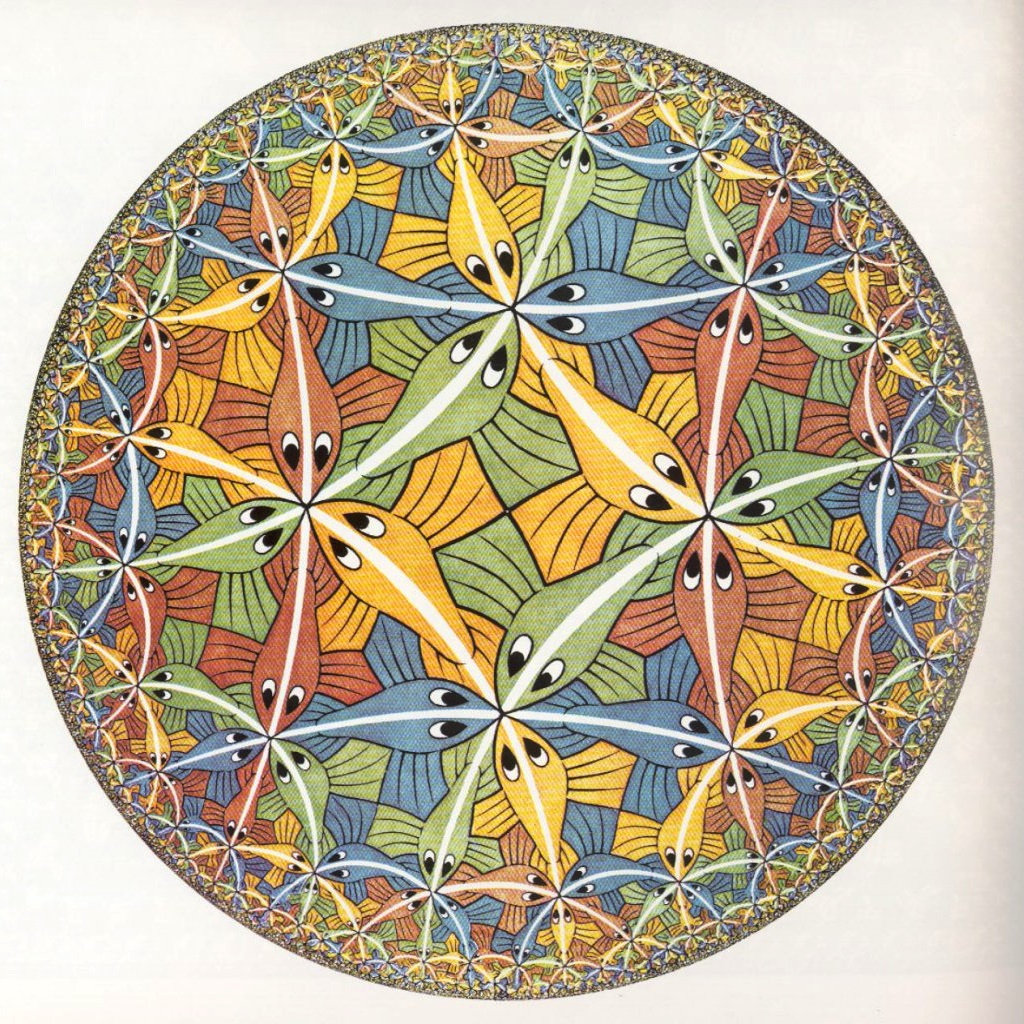
\includegraphics[width=0.55\linewidth]{figures/circlelimit3.jpg}\\[0.6em]
{\small Figure 3: M. C. Escher's \emph{Circle Limit III} (1959).}
\end{center}

\noindent Let us use the methods of the calculus of variations
to find the hyperbolic geodesics, which are the
``straight lines'' (actually shortest paths) between
two points $(x_1,y_1), (x_2,y_2)$ in the hyperbolic
plane. Imitating the setup of the plane geodesics
example, we are trying to minimize the functional

\begin{align*}
\Phi_{\mathbb{H}} = \int_{x_1}^{x_2} \,ds = \int_{x_1}^{x_2} \frac{\sqrt{1+q'(x)^2}}{q}\,dx
= \int_{x_1}^{x_2} L_{\mathbb{H}}(q',q)\,dx,
\end{align*}

\noindent which is expressed in terms of a Lagrangian

\begin{align*}
L_{\mathbb{H}}(q',q) = \frac{\sqrt{1+q'^2}}{q}.
\end{align*}

\noindent The Euler-Lagrange equation becomes

\begin{align*}
\frac{d}{dx}\left(\frac{q'(x)}{q(x)\sqrt{1+q'(x)^2}}\right)=
\frac{d}{dx}\left(\frac{\partial L_{\mathbb{H}}}{\partial q'} \right) = \frac{\partial L_{\mathbb{H}}}{\partial q} = -\frac{\sqrt{1+q'(x)^2}}{q(x)^2}.
\end{align*}

\noindent After a short computation, this reduces to the
equation

\begin{align*}
1+q'(x)^2+q(x)q''(x) = 0,
\end{align*}

\noindent or

\begin{align*}
\frac{d^2}{dx^2}\left(\tfrac12 q(x)^2\right)
= \frac{d}{dx}\left(q(x) q'(x)\right) = -1.
\end{align*}

\noindent This is readily integrated, to give

\begin{align*}
\tfrac12 q(x)^2 = -x^2 + Cx + D,
\end{align*}

\noindent or

\begin{align*}
q(x) = \sqrt{a^2 - (x-b)^2},
\end{align*}

\noindent where $D=a^2-b^2, C=2b$. The equation $y=q(x)$ is the
equation for a semicircular arc that crosses the
$y$-axis perpendicularly --- these semicircular arcs
are the geodesics in the hyperbolic plane. In
addition, in the case when $x_1=x_2$, it is easy to
verify that the geodesic connecting $(x_1,y_1)$ to
$(x_2,y_2)$ will be a vertical straight line. (In the
``unit disk'' version of the hyperbolic plane, the
geodesics are circular arcs that intersect the
boundary of the disk perpendicularly.)
\end{example}

\begin{xexercise}
Find a formula for the length (as measured using the
hyperbolic metric!) of a hyperbolic geodesic arc
between the points
$(x_1,y_1), (x_2,y_2)\in \mathbb{H}$.
\end{xexercise}

\begin{example}[Isoperimetric inequality]
The \emph{isoperimetric problem} was the classical
problem, discussed already by the ancient Greeks, of
finding the simple closed curve in the plane with
perimeter $L$ that bounds the largest area (in modern
times the problem has been considerably generalized to
higher dimensions, curved spaces etc.). The answer is
that the so-called \emph{isoperimetric curve} is a circle,
and can be derived using the calculus of variations. A
slight complication is that the problem involves
minimizing a functional (the area bounded by the
curve) subject to a constraint (representing the fixed
perimeter); this difficulty can be addressed easily
using the standard idea of Lagrange multipliers from
``ordinary'' calculus (note the repeated occurrence of
the mathematician Joseph Louis Lagrange's name --- it
is no coincidence, of course).

We model the isoperimetric problem as the problem of
minimizing the area functional

\begin{align*}
A = \int_{x_0}^{x_1} q(x)\,dx
\end{align*}

\noindent among all curves $q(x)$ taking nonnegative values on
$[x_0,x_1]$, and satisfying $q(x_0)=q(x_1)=0$ as well
as the arc length constraint

\begin{align*}
\int_{x_0}^{x_1} ds =  \int_{x_0}^{x_1} \sqrt{1+q'(x)^2}\,dx = \ell.
\end{align*}

\noindent Such a curve $q(x)$ represents the ``upper part'' of
the closed curve that lies above the $x$-axis, and
meets it at the points $x=x_0, x=x_1$. The solution
should be a semicircle meeting the $x$-axis
perpendicularly at those points; once this fact is
derived, one can derive the claim about circles being
the solution to the isoperimetric problem without too
much effort, after making reasonable assumptions about
the form of the solution.

Since this is an optimization problem under
constraints, the technique of Lagrange multipliers
requires us to solve the modified \emph{non-constrained}
problem of optimizing the functional

\begin{align*}
A_\lambda = \int_{x_0}^{x_1} q(x) + \lambda \sqrt{1+q'(x)^2}\,dx
= \int_{x_0}^{x_1} L_\lambda(q',q)\,dx,
\end{align*}

\noindent where $L_\lambda$ is a new Lagrangian that is
obtained by taking the ``original'' Lagrangian $L=q$
and adding a constant multiple of the constraint
function $\sqrt{1+q'^2}$. The price of replacing the
constrained problem by an unconstrained one is the
introduction of an additional parameter, $\lambda$,
known as the \emph{Lagrange multiplier}. After solving the
unconstrained problem in terms of the parameter
$\lambda$, the requirement for the constraint to be
satisfied gives an equation for $\lambda$. (A proof
that this technique works is beyond the scope of this
course, but the geometric intuition is very similar to
the case of Lagrange multipliers in ordinary
calculus.)

To see how this idea works in practice, we write the
Euler-Lagrange equation
$\frac{d}{dx}\left(\frac{\partial L_\lambda}{\partial
q'}\right) = \frac{\partial L_\lambda}{\partial q}$
for the unconstrained optimization problem. This gives

\begin{align*}
\frac{d}{dx}\left( \frac{\lambda q'(x)}{\sqrt{1+q'(x)^2}}\right) = 1,
\end{align*}

\noindent or

\begin{align*}
\frac{q'(x)^2}{1+q'(x)^2} = (Ax+B)^2,
\end{align*}

\noindent where $A,B$ are constants related to the values of
$\lambda$ and an integration constant. Solving for
$q'$ and then integrating, we get

\begin{align*}
q'(x) &= \pm \frac{Ax+B}{\sqrt{1-(Ax+B)^2}}, \\
q(x) &= \pm \sqrt{A^{-1}-(x+B/A)^2}+E = \pm \sqrt{C-(x+D)^2} + E,
\end{align*}

\noindent where $C,D,E$ are constants. If we now impose the
constraints that $q$ is nonnegative,
$q(x_0)=q(x_1)=0$, and assume that the arc length
$\ell$ is exactly $\frac{\pi}{2}(x_1-x_0)$, we find
that the solution to our optimization problem must
have the form

\begin{align*}
q(x) = \sqrt{\left(\frac{x_1-x_0}{2}\right)^2 - \left(x-\frac{x_1+x_0}{2}\right)^2},
\end{align*}

\noindent which is indeed a semicircular arc that meets the
$x$-axis perpendicularly at $x_0,x_1$.
\end{example}

\begin{xexercise}[Surfaces of revolution]
The surface obtained by taking a curve $y=q(x)$ on
some interval $[x_1,x_2]$ and rotating it around the
$x$-axis is called the \emph{surface of revolution} of the
curve. Its surface area is known to be

\begin{align*}
S = \int_{x_1}^{x_2} 2\pi y\,ds = 2\pi \int_{x_1}^{x_2} q(x)\sqrt{1+q'(x)^2}\,dx.
\end{align*}

\noindent For given values of $x_1<x_2$ and boundary values
$q(x_1)=y_1, q(x_2)=y_2$, find the nonnegative curve
that minimizes $S$. The surface of revolution of this
famous curve can be physically realized as the shape
of a soap film between two circular metal rings (see
Figure 4).
\end{xexercise}

\begin{center}
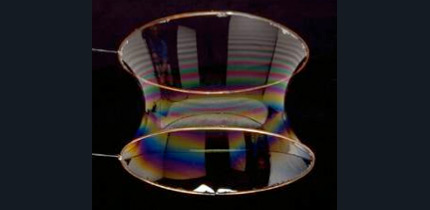
\includegraphics[width=0.55\linewidth]{figures/catenoid.jpg}\\[0.6em]
{\small Figure 4: The catenoid, a minimal surface of
revolution.}
\end{center}

\begin{xexercise}[A hanging rope]
A rope of length $L$ and uniform linear density $\rho$
hangs between two points $\mathbf{A}=(x_1,y_1)$,
$\mathbf{B}=(x_2,y_2)$, where $x_1<x_2$, and clearly
we have to assume that
$(x_2-x_1)^2+(y_2-y_1)^2 \le L^2$. Its shape is
determined by the requirement that the potential
energy

\[
E = -\int_{x_1}^{x_2} \rho gy\,ds
\]

\noindent is minimized. Find the general equation for the
shape.
\end{xexercise}

\begin{example}[The elastic rod]
A thin elastic rod of length $L$ is made to bend as
it is clamped horizontally between the two points
$(0,0)$ and $(A,0)$ (where $A<L$). Its shape can be
determined from the condition that the elastic energy
is minimized. The energy is proportional to an
integral along the curve of the square of its
curvature:

\[
E = \int \tfrac12 J (\textrm{curvature})^2\,ds = \tfrac12 J \int \kappa(s)^2 \,ds,
\]

\noindent where $J$ is a constant characteristic of the
material and geometric cross section of the rod, and
$ds$ denotes arc length. The curvature $\kappa(s)$ at
a point along the curve is the reciprocal of the
\emph{radius of curvature}, defined as the radius of a
circle that can be brought to touch the curve
tangentially in such a way that both the first and
second derivatives of the curve and circle coincide.

Let the shape of the rod be described by the
functions $(x(s), y(s))$ of the arc length parameter
$s$, which varies from $0$ to $L$. Let
$\theta=\theta(s)$ be the angle between the positive
$x$-axis and the tangent to the curve at the point
$(x(s),y(s))$; i.e., we have the relations

\begin{align*}
\tan \theta = \frac{dy}{dx}, \quad \cos\theta = \frac{dx}{ds}, \quad \sin\theta = \frac{dy}{ds}.
\end{align*}

\noindent From elementary geometry it is known that
$\kappa(s) = |\frac{d\theta}{ds}|$, i.e., the
curvature is the absolute rate of change of the angle
of the tangent with arc length [it is also the
magnitude of the acceleration vector
$(x''(s),y''(s))$]. So, in terms of the
angle-arc-length functional representation $\theta(s)$
of the curve, the energy functional can be written as

\begin{align*}
E = \int_0^L \tfrac12 J \theta'(s)^2 \,ds.
\end{align*}

\noindent To derive an ODE for this minimization problem, note
that the boundary conditions

\begin{align*}
y(0) = y(L) = x(0)= 0, \ \ \ x(L)=A,
\end{align*}

\noindent translate to two constraints

\begin{align*}
\int_0^L \frac{dy}{ds}\,ds = \int_0^L \sin\theta(s)\,ds &= 0, \\
\int_0^L \frac{dx}{ds}\,ds = \int_0^L \cos\theta(s)\,ds &= A.
\end{align*}

\noindent In addition, we have the condition
$\theta(0)=\theta(L)=0$. We therefore need to
introduce two Lagrange multipliers
$\lambda_1, \lambda_2$, and solve the unconstrained
optimization problem for the modified energy
functional

\begin{align*}
E_{\lambda_1, \lambda_2} = \int_0^L \left(\tfrac12 J \theta'(s)^2 - \lambda_1 \sin\theta(s) - \lambda_2 \cos\theta(s)\right)\,ds
\end{align*}

\noindent This gives the Euler-Lagrange equation

\begin{equation*} \tag{17}\label{eq:elasticaeq}
\begin{split}
J \theta''(s) = -\lambda_1 \cos \theta(s) + \lambda_2 \sin\theta(s).
\end{split}
\end{equation*}

\noindent Note that this equation is somewhat similar to the
pendulum equation \eqref{eq:pendulumeq}, and indeed can be
brought to the form of \eqref{eq:pendulumeq} by replacing
the function $\theta(s)$ by a shifted version of it
$\varphi(s)=\theta(s)+\alpha$, for a suitable
$\alpha$. The curves solving \eqref{eq:elasticaeq} are
known as \emph{elastica} curves, and this useful
coincidence between the elastica equation and the
theory of the pendulum is the starting point for a
beautiful analysis of the possible shapes that can be
assumed by an elastic rod. We will not go into the
details of this analysis here.
\end{example}

\begin{xexercise}[Solid of revolution with least airflow resistance]
The air resistance experienced by a bullet, whose
shape is the solid of revolution of a curve $y=q(x)$,
moving through the air is

\begin{align*}
\Phi = 4\pi \rho v^2 \int_0^L q(x) q'(x)^3\,dx,
\end{align*}

\noindent where $\rho$ is the density of the material, $v$ is
the velocity of motion and $L$ is the length of the
body of the bullet. Find the optimal shape $q(x)$
that results in the smallest resistance, subject to
the conditions $q(0)=0, q(L)=R$.
\end{xexercise}

\section{The phase flow and Liouville's theorem}

Hamiltonian systems often have quantities which are
conserved; for example, in autonmous systems we saw
that the Hamiltonian itself is conserved. In other
cases, if the Lagrangian does not depend on one of the
generalized coordinates $q_j$, then
$\frac{\partial L}{\partial q_j}=0$, so, by the
Euler-Lagrange equation for that coordinate, the
generalized momentum
$p_j = \frac{\partial L}{\partial \dot{q}_j}$ is a
conserved quantity (in such a case we say that $q_j$
is a \emph{cyclic coordinate}). Such invariant quantities
lead directly to the usual conservation laws from
mechanics --- the conservation of energy, of momentum,
and of angular momentum --- as well as to more exotic
conserved quantities that arise in specific problems.

We now discuss a different kind of conserved
quantity, one that is associated not with specific
solutions, but rather with an entire family of
solutions. What we will do is to start with an entire
set of initial states in the phase space, then let
those states evolve according to the dynamical
equations. After some time $t$, the initial states
have evolved to occupy some new set in the phase
space. It turns out that the total \emph{area} of the set
is conserved: this is the statement of Liouville's
theorem.

To state the theorem formally, given a Hamiltonian
system \eqref{eq:hamiltoniansystem}, for each point
$\mathbf{x}=(p_0,q_0)\in\mathbb{R}^2$ and time
$t\ge 0$, denote by $\varphi_t(\mathbf{x})$ the point
$(p(t),q(t))$, where $(p(t),q(t))$ are the solutions
to the equations \eqref{eq:hamiltoniansystem} with initial
condition $p(0)=p_0, q(0)=q_0$. (We assume that the
system is such that the solutions exist for all time
$t\ge 0$.) Thus, for each $t\ge 0$ we have
constructed a mapping

\[
\varphi_t:\mathbb{R}^2\to\mathbb{R}^2,
\]

\noindent which takes a ``present'' point corresponding to the
state of the system at time $0$ into a ``future''
point corresponding to the state of the system $t$
units of time later. The family of maps
$(\varphi_t)_{t\ge 0}$ is called the \emph{phase flow} of
the system: it describes how points ``flow'' along the
solution lines of the system.

\begin{thm}[Liouville's theorem]
The phase flow preserves area. More precisely, given
a region $E\subset\mathbb{R}^2$ with finite area, for
any $t\ge 0$ we have

\begin{align*}
\operatorname{area}(\varphi_t(E)) = \operatorname{area}(E).
\end{align*}

\end{thm}

\begin{proof}
Note that for fixed $t$, there is a one-to-one
correspondence between points $(p,q) \in \varphi_t(E)$
and points $(p_0,q_0)\in E$, defined by
$(p,q)=\varphi_t(p_0,q_0)$. This smooth map has a
Jacobian

\begin{align*}
J_t = \frac{\partial (p,q)}{\partial (p_0,q_0)},
\end{align*}

\noindent i.e., $J_t$ is the determinant of the Jacobian matrix

\begin{align*}
\frac{D(p,q)}{D(p_0,q_0)} = \left(\begin{array}{cc}
\frac{\partial p}{\partial p_0} & \frac{\partial p}{\partial q_0} \\ \frac{\partial q}{\partial p_0} & \frac{\partial q}{\partial q_0}
\end{array}\right).
\end{align*}

\noindent The Jacobian factor $J_t$ enters into the area
computation via a change of variables in a double
integral, as follows:

\begin{align*}
\operatorname{area}(\varphi_t(E)) &= \iint_{\varphi_t(E)} dp\,dq
= \iint_E \frac{\partial (p,q)}{\partial (p_0,q_0)}\,dp_0\,dq_0 \\
&= \iint_E J_t \,dp_0\,dq_0.
\end{align*}

\noindent We claim that $J_t\equiv 1$ for all $t$. This will
imply that

\begin{align*}
\operatorname{area}(\varphi_t(E)) &= \iint_{\varphi_t(E)} dp\,dq
= \iint_E \,dp_0\,dq_0 = \operatorname{area}(E),
\end{align*}

\noindent and therefore finish the proof. It will be
instructive to do this by computing $J_t$ more
generally for the generic (not necessarily
Hamiltonian) planar system

\begin{align*}
\dot{p} = F(p,q,t), \qquad
\dot{q} = G(p,q,t).
\end{align*}

\noindent Denote

\begin{align*}
X_t = \frac{D(p,q)}{D(p_0,q_0)} = \left(\begin{array}{cc}
\frac{\partial p}{\partial p_0} & \frac{\partial p}{\partial q_0} \\ \frac{\partial q}{\partial p_0} & \frac{\partial q}{\partial q_0}
\end{array}\right),
\end{align*}

\noindent and observe that, by the chain rule,

\begin{align*}
\frac{dX_t}{dt} =
\left(\begin{array}{cc}
\frac{\partial \dot{p}}{\partial p_0} & \frac{\partial \dot{p}}{\partial q_0} \\ \frac{\partial \dot{q}}{\partial p_0} & \frac{\partial \dot{q}}{\partial q_0}
\end{array}\right) =
\left(\begin{array}{cc}
\frac{\partial p}{\partial p_0} \frac{\partial F}{\partial p} + \frac{\partial q}{\partial p_0} \frac{\partial F}{\partial q} & \frac{\partial p}{\partial q_0} \frac{\partial F}{\partial p} + \frac{\partial q}{\partial q_0} \frac{\partial F}{\partial q} \\
\frac{\partial p}{\partial p_0} \frac{\partial G}{\partial p} + \frac{\partial q}{\partial p_0} \frac{\partial G}{\partial q} & \frac{\partial p}{\partial q_0} \frac{\partial G}{\partial p} + \frac{\partial q}{\partial q_0} \frac{\partial G}{\partial q}
\end{array}\right)
= A_t X_t,
\end{align*}

\noindent where

\begin{align*}
A_t = A_t(p_0,q_0) = \left(\begin{array}{cc} \frac{\partial F}{\partial p} & \frac{\partial F}{\partial q} \\ \frac{\partial G}{\partial p} & \frac{\partial G}{\partial q} \end{array}\right).
\end{align*}

\noindent In other words, for fixed $(p_0,q_0)$, the matrix
$X_t$ satisfies the time-dependent linear matrix ODE

\begin{align*}
\dot{X}_t = A_t X_t,
\end{align*}

\noindent with the initial condition $X_0 = I$ (the $2\times2$
identity matrix).

As a consequence, we now claim that the determinant
$J_t = \det X_t$ also satisfies an ODE, namely

\begin{equation*} \tag{18}\label{eq:liou-jac-ode}
\begin{split}
\dot{J}_t = \operatorname{tr}(A_t) J_t.
\end{split}
\end{equation*}

\noindent Indeed, for small positive $h>0$ we have

\begin{align*}
J_{t+h} &= \det(X_{t+h}) = \det( X_t+h A_t X_t + O(h^2) ) \\
&= \det((I+h A_t)X_t+O(h^2))
= \det(I+h A_t) \det(X_t) + O(h^2) \\
&= (1 + h \operatorname{tr}(A_t)) J_t + O(h^2),
\end{align*}

\noindent where the last step is true because of the exercise
below on determinants of perturbations of the identity
matrix. Subtracting $J_t$ from both sides and taking
the limit as $h\downarrow 0$ gives

\begin{align*}
\frac{dJ_t}{dt} = \lim_{h\downarrow 0} \frac{J_{t+h}-J_t}{h} =
\lim_{h\downarrow 0} \left(\operatorname{tr}(A_t)J_t + O(h)\right) = \operatorname{tr}(A_t)J_t.
\end{align*}

\noindent The equation \eqref{eq:liou-jac-ode} is an easy scalar
ODE for $J_t$, with the initial condition $J_0=1$.
Its solution is

\begin{equation*} \tag{19}\label{eq:liouville-jacobian}
\begin{split}
J_t &= \exp\left( \operatorname{tr}\left(\int_0^t A_s\,ds\right)\right) \\
&= \exp\left[ \int_0^t \left(\frac{\partial F}{\partial p}+\frac{\partial G}{\partial q}\right)\,ds \right] \\
&= \exp\left( \int_0^t \operatorname{div}(F,G) \,ds \right).
\end{split}
\end{equation*}

\noindent Going back to the case of the Hamiltonian system, we
recall that in this case

\[
\operatorname{div} (F,G) = \frac{\partial F}{\partial p}+\frac{\partial G}{\partial q} = -\frac{\partial^2 H}{\partial p \partial q} +
\frac{\partial^2 H}{\partial p \partial q} = 0,
\]

\noindent so we finally get that $J \equiv 1$, as claimed.
\end{proof}

\begin{xexercise}[Determinants of perturbations of the identity matrix]
Show that if $A$ is a square matrix then

\begin{align*}
\frac{d}{dh}\Big|_{h=0} \det(I+h A) = \operatorname{tr}(A),
\end{align*}

\noindent or equivalently

\begin{align*}
\det(I+h A) = 1 + h \operatorname{tr}(A) + O(h^2).
\end{align*}

\end{xexercise}

\begin{xexercise}[Matrix exponentials]
The exponential $\exp(A)$ of a square matrix
$A=(a_{i,j})_{i,j=1}^d$ is defined by

\begin{align*}
\exp(A) = \sum_{n=0}^\infty \frac{1}{n!} A^n.
\end{align*}

\begin{enumerate}[label=\arabic*.]
\item Show that the series converges absolutely in the
matrix norm

\begin{align*}
\lVert A \rVert = \sum_{i,j} |a_{i,j}|.
\end{align*}

\item Show that the unique solution to the linear vector
ODE

\begin{align*}
\dot{\mathbf{x}} = A \mathbf{x}
\end{align*}

\noindent with initial condition $\mathbf{x}(0) = \mathbf{x}_0$
(where we think of $\mathbf{x}$ as a column vector in
$\mathbb{R}^d$) can be expressed in terms of matrix
exponentials, namely

\begin{align*}
\mathbf{x}(t) = \exp\left(t \mathbf{A}\right) \mathbf{x}_0, \qquad t\ge 0.
\end{align*}

\item Use this to explain the characterization of the
stability of rest points in a planar system in terms
of the eigenvalues of the Jacobian matrix.

\item Prove that if $A, B$ are commuting square matrices
(i.e., matrices which satisfy $AB=BA$) then
$\exp(A+B)=\exp(A)\exp(B)$.
\end{enumerate}

\end{xexercise}

\begin{xexercise}[Determinant of a matrix exponential]
Prove the formula

\begin{align*}
\det\left( \exp(A)\right) = e^{\operatorname{tr}(A)},
\end{align*}

\noindent where $A$ is a square matrix and
$\operatorname{tr}(A)$ denotes the trace of $A$.

$\textbf{Hint.}$ Take determinants of both sides of
the equation $\exp(A)=\exp(n^{-1} A)^n$, which is
true by part (4) of the exercise above, then use the
fact that $\exp(n^{-1} A)=I+n^{-1}A + O(n^{-2})$ and
the exercise above on determinants of matrices close
to $I$.
\end{xexercise}

\begin{cor}
The phase flow of a planar system preserves area if
and only if the system is Hamiltonian.
\end{cor}

\begin{proof}
We saw in the proof of Liouville's theorem that the
preservation of area is determined by the Jacobian
$J_t$ of the phase flow: if $J_t \equiv 1$ then the
system preserves area; conversely, if $J_t(p,q)\neq 1$
for some $t$ at a point $(p,q)=\varphi_t(p_0,q_0)$,
then a small disk of radius $\epsilon$ and area
$\pi \epsilon^2$ around $(p_0,q_0)$ is mapped by
$\varphi_t$ to a set of area approximately
$\pi \epsilon^2 J_t \neq \pi \epsilon^2$, and
therefore the phase flow does not preserve area.

To conclude, from the computation in
\eqref{eq:liouville-jacobian} it follows that the system
preserves area if and only if
$\operatorname{div}(F,G)=0$, and we already showed in
\hyperref[lem:hamiltonian-div]{Lemma~\ref*{lem:hamiltonian-div}} that this is equivalent to
the system being Hamiltonian.
\end{proof}

\begin{cor}
The rest points of an autonomous Hamiltonian system
are either saddle points or centers.
\end{cor}

\begin{proof}
An asymptotically stable or unstable rest point
(which is either a node or a spiral) would imply that
the phase flow either contracts or expands small disks
around the rest point; by Liouville's theorem, this is
impossible.
\end{proof}

\section{Poincaré recurrence theorem}

Liouville's theorem is the starting point for a set
of important investigations into the qualitative
behavior of Hamiltonian systems. The following theorem
illustrates the kind of conclusions that the theorem
will enable us to draw.

\begin{thm}[Poincaré recurrence theorem]
\label{thm:poincare-recurrence}
Let $D$ be a bounded region of the plane. Let
$\varphi:D\to D$ be a continuous one-to-one map which
is area-preserving. Then in any neighborhood
$N\subset D$, there exists a point
$\mathbf{p}=(p,q) \in N$ such that the sequence of
points $(\varphi^k(\mathbf{p}))_{k=0}^\infty$ returns
to $N$ infinitely many times. Here,
$\varphi^k(\mathbf{p})$ denotes the \emph{$k$th iterate of
$\varphi$}, i.e.,
$\varphi^2(\mathbf{p})=\varphi(\varphi(\mathbf{p})),
\varphi^3(\mathbf{p})=\varphi(\varphi(\varphi(\mathbf{p})))$,
etc.
\end{thm}

\begin{proof}
The images of the neighborhood $N$ under $\varphi$
are

\begin{align*}
N, \varphi(N), \varphi^2(N), \varphi^3(N), \ldots
\end{align*}

\noindent Since $\varphi$ preserves areas, these are all sets
of equal area, which lie in the bounded region $D$.
It follows that there must be two of them which
intersect (otherwise the total area would be
infinite), that is, we have
$\varphi^k(N) \cap \varphi^\ell(N) \neq \emptyset$
for some $k>\ell\ge 0$. If
$\mathbf{p}_1, \mathbf{p}_2 \in N$ are two points
such that
$\varphi^\ell(\mathbf{p}_1)=\varphi^k(\mathbf{p}_2)=\varphi^\ell(\varphi^{k-\ell}(\mathbf{p}_2))$,
then, since $\varphi$ is one-to-one, we get that
$\varphi^{k-\ell}(\mathbf{p}_2)=\mathbf{p}_1$. We
have shown that there is a point $\mathbf{p}_2\in N$
and an integer $j>0$ such that
$\varphi^j(\mathbf{p}_2)\in N$, i.e., the point
returned to $N$ after $j$ iterations. To prove the
stronger claim that there is a point that returns to
$N$\emph{infinitely many times}, the idea is to apply the
same argument again, replacing $N$ with
$N\cap \varphi^j(N)$. This is left as an exercise to
the reader.
\end{proof}

\noindent In the context of an autonomous Hamiltonian system,
\hyperref[thm:poincare-recurrence]{Theorem~\ref*{thm:poincare-recurrence}} becomes applicable
(by taking $\varphi=\varphi_s$ for any fixed $s>0$)
when there is a set of trajectories that is known to
be bounded; for example, trajectories with energy
bounded from above in such a way that we know no
trajectory can escape to infinity. The conclusion in
this case is that in the vicinity of each state of the
system included in the bounded region, there are
states which, after evolving for some time, will
return to the vicinity of the same state.

It should be noted that in all but the simplest
possible systems, it is hopeless to solve the
equations analytically. Many systems, such as the
double pendulum, exhibit an additional complexity to
their behavior, known as \emph{chaos}, which makes them
even more difficult to analyze in detail. Thus, in
many cases obtaining a rough understanding of the
system's behavior, using qualitative results such as
the Poincaré recurrence theorem, is our only hope.
Note that Liouville's theorem also holds for
Hamiltonian systems with more than one degree of
freedom (we will not prove this, but the proof is not
much more difficult than the planar case).

\section{Liouville's theorem and ``statistical dynamics''}

Another, more quantitative, way in which Liouville's
theorem makes it possible to reach a broad
understanding of a complicated nonlinear system
without being able to describe in detail specific
solutions, is by looking at \emph{statistical} behavior. To
be more concrete, if $\mathbf{p}(t)$ is a solution
curve in $\mathbb{R}^d$ of an autonomous Hamiltonian
system with $d$ degrees of freedom, instead of trying
to understand in detail the motion of $\mathbf{p}(t)$
through the phase space, we can simply ask about the
frequency of time $\mathbf{p}(t)$ spends in any given
part of it. That is, for a well-behaved (say, bounded
and open) set $A \subseteq \mathbb{R}^2$, we look at
the time average

\begin{align*}
f_A(T) = \frac{1}{T} \int_0^T 1_{\{ \mathbf{p}(t) \in A\}}\,dt,
\end{align*}

\noindent where the integrand is equal to $1$ if
$\mathbf{p}(t)\in A$ or $0$ otherwise, and ask
whether this quantity (which might be called the
\emph{empirical frequency of visits to $A$}) might
converge to an interesting limit (which will be a
function of the set $A$) as $T\to\infty$. An ideal
situation is one in which the limit does not depend on
the initial condition $\mathbf{p}(0)$, and looks like

\begin{equation*} \tag{20}\label{eq:idealdensity}
\begin{split}
\lim_{T\to\infty} f_A(T) = f_A^{(\infty)} := \int_A g(\mathbf{p})\,d\mathbf{p}.
\end{split}
\end{equation*}

\noindent In this case we will say that the density
$g(\mathbf{p})$ describes in some sense the ``ideal''
statistics of the system: by following the trajectory
of a single solution for a long time, we will learn
about the relative proportion of time spent in each
part of the phase space by \emph{any} solution. Such
knowledge may have very practical applications. Can we
say what the density $g(\mathbf{p})$ might be? Note
that the function $f_A^{(\infty)}$ by its definition
ought to be invariant under the phase flow, in the
sense that for all $t\ge 0$,

\begin{align*}
f_A^{(\infty)} = f_{\varphi_t(A)}^{(\infty)}
\end{align*}

\noindent (an exercise to the reader: prove this). Liouville's
theorem says that $A$ and $\varphi(A)$ have the same
volume, i.e.,

\begin{align*}
\int_A d\mathbf{p} = \int_{\varphi_t(A)} d\mathbf{p},
\end{align*}

\noindent so it is reasonable to guess that if
\eqref{eq:idealdensity} holds then the density
$g(\mathbf{p})$ might simply be a constant. Again, if
a result of this type were true it would give us a
very nice and potentially useful insight into the
behavior of the system. It turns out that
\eqref{eq:idealdensity} in its literal form cannot be
true, for the simple reason that the system has a
natural conserved quantity, the Hamiltonian (which
here for convenience we will call the energy); so,
each solution only gets to explore a part of the phase
space with a constant energy, and therefore the limit
on the right-hand side of \eqref{eq:idealdensity} cannot
be independent of the initial condition and must
instead necessarily be a function of the initial
energy. However, there is a way to work around this
slight complication and it does not detract from the
usefulness of the statistical approach to analyzing
dynamical systems. In fact, the argument we just
sketched is the beginning of an area of mathematics
called \emph{ergodic theory}, which we will discuss more in
detail in the second part of the course.

\section{The pendulum equation, falling trees and domino waves}

In this section we show how to obtain an exact
solution of the simple pendulum equation

\begin{align*}
\ddot{\theta} + \frac{g}{\ell} \sin \theta = 0
\end{align*}

\noindent and show several applications of this solution.
Unfortunately, the solution involves some exotic
special functions that are unfamiliar to most people
(possibly even to most mathematicians!) --- the
elliptic integrals and Jacobi elliptic functions ---
but it is useful (and entertaining) nonetheless.

\subsection{Analytic solution using elliptic integrals}

We derive the solution under the assumption that
$\theta(0) = 0$, $\dot{\theta}(0)>0$. Let
$\lambda=g/\ell$, so the equation becomes
$\ddot{\theta}+\lambda \sin \theta=0$. Conservation
of energy gives the equation

\begin{equation*} \tag{21}\label{eq:pendulum-energy-cons}
\begin{split}
\tfrac12 \dot{\theta}^2-\lambda \cos \theta = \textrm{const}
\end{split}
\end{equation*}

\noindent (to verify this, differentiate both sides). For
reasons which will become clear soon, denote the
integration constant on the right by
$\lambda(2k^2-1)$, where $k\ge0$ and use the relation
$\cos \theta = 1-2\sin^2\tfrac{\theta}{2}$. This
brings \eqref{eq:pendulum-energy-cons} to the form

\begin{equation*} \tag{22}\label{eq:pendulum-energy-cons2}
\begin{split}
(\dot{\theta})^2 = 4\lambda \left(k^2-\sin^2 \tfrac{\theta}{2} \right).
\end{split}
\end{equation*}

\noindent Note that this already makes it easy to plot the
phase portrait (in the $\theta$-$\dot{\theta}$ plane,
or wrapped around a cylinder, since adding multiples
of $2\pi$ to $\theta$ does not change the physical
state of the system); see Figure 5.

\begin{center}
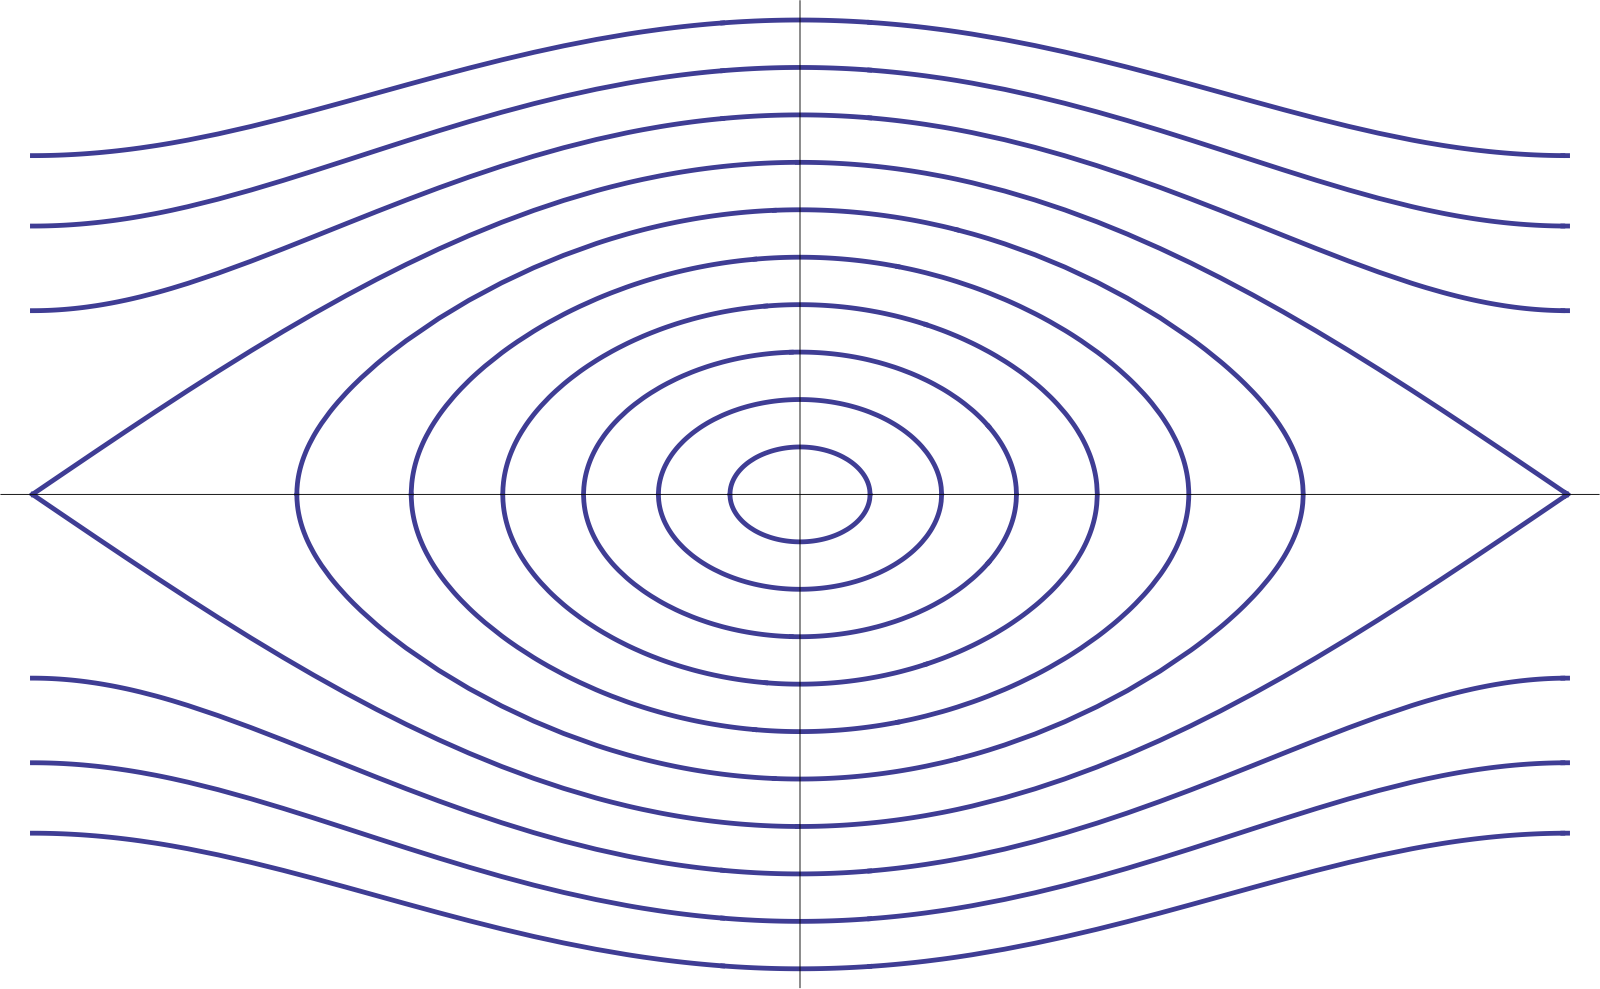
\includegraphics[width=0.52\linewidth]{figures/pendulumphasediag.png}\hspace{0.02\linewidth}%
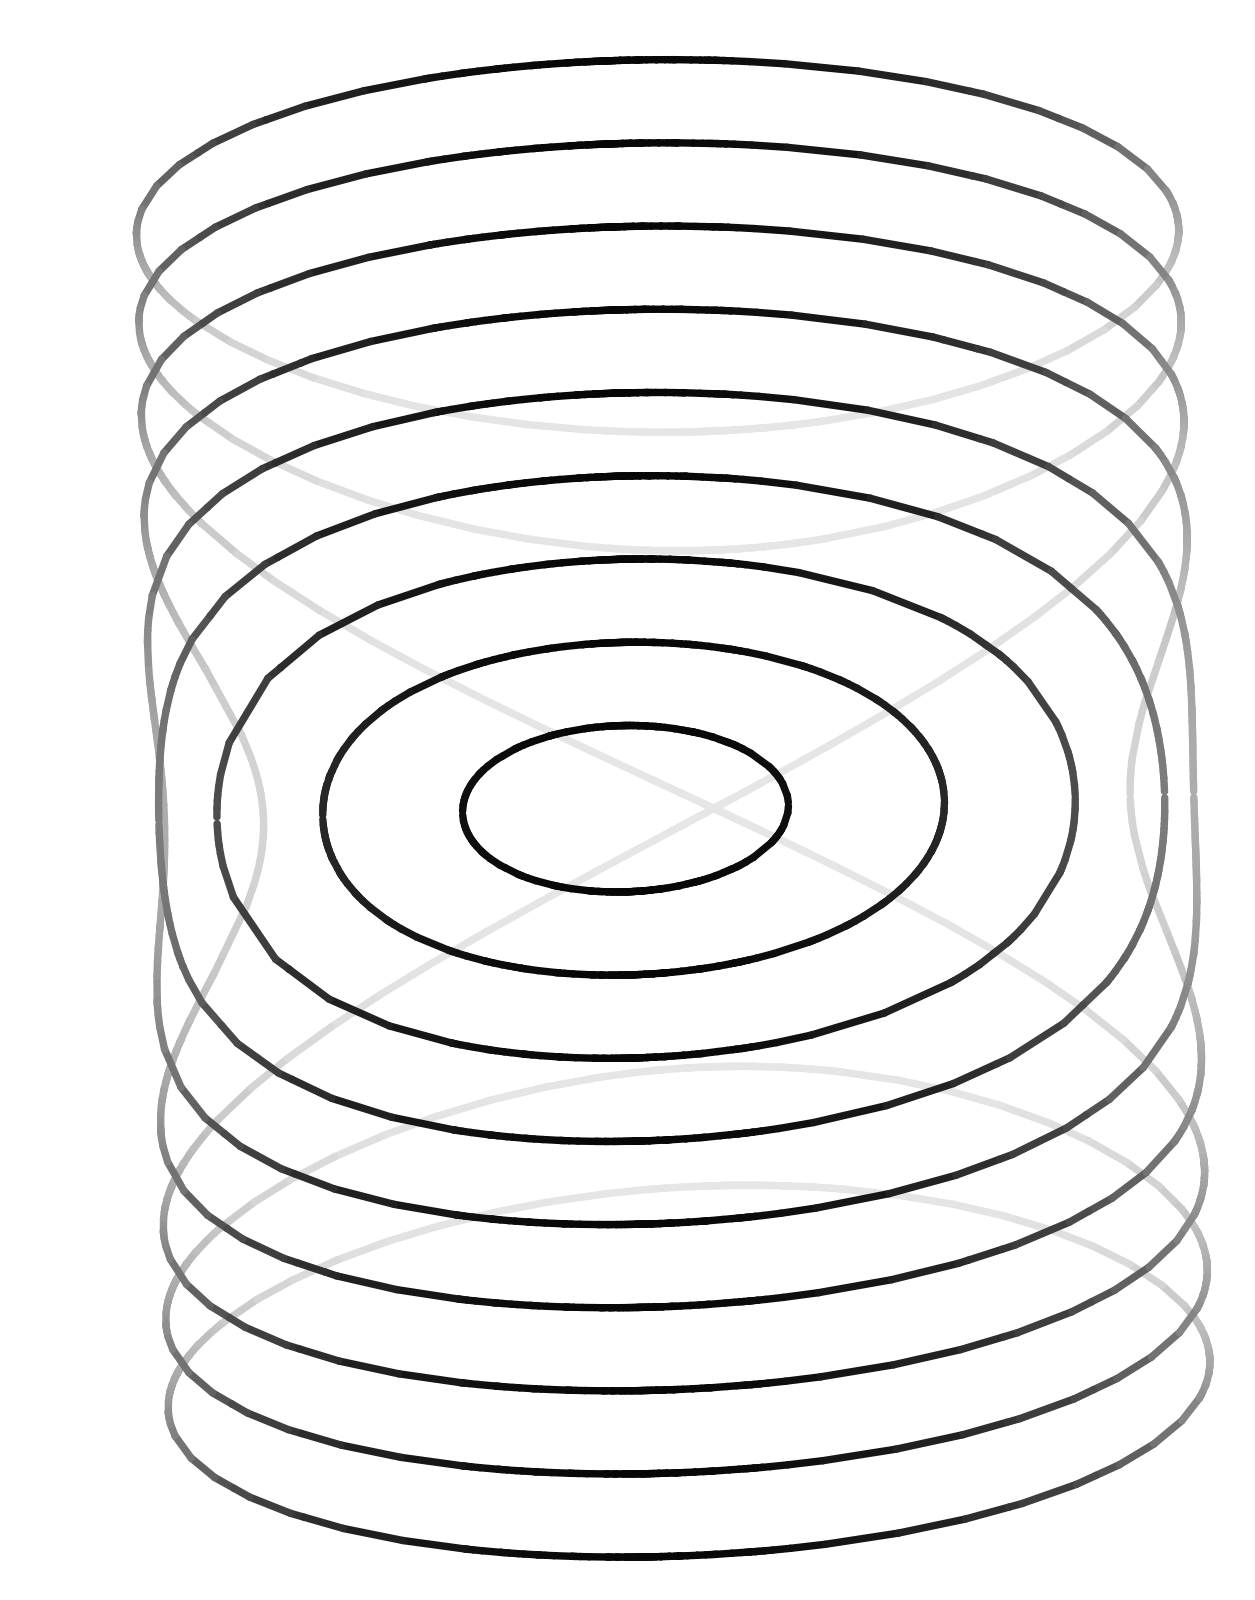
\includegraphics[width=0.30\linewidth]{figures/pendulumphasediag3d.png}\\[0.6em]
{\small Figure 5: The phase portrait of the simple pendulum:
in the planar representation, the constant energy
curves are given by the equation
$y=\pm 2 \sqrt{\lambda\left(k^2-\sin^2(x/2)\right)}$
for different values of $k$.}
\end{center}

\noindent The relation between the parameter $k$ and the
initial angular velocity $\dot{\theta}(0)$ is found
by setting $t=0$ in \eqref{eq:pendulum-energy-cons2},
giving

\begin{align*}
k=\frac{1}{2\sqrt{\lambda}} \dot{\theta}(0).
\end{align*}

\noindent It is also easy to see from the energy conservation
equation \eqref{eq:pendulum-energy-cons2} that the
periodic solutions (which are the solutions for which
$\theta$ remains bounded) correspond to $0<k<1$, and
that in that case we have
$k=\sin (\theta_{\textrm{max}}/2)$ where
$\theta_{\textrm{max}}=\sup_{t\ge 0} \theta(t)$ is
the maximal angle that the pendulum will reach (or
approach asymptotically, in the case
$\theta_{\textrm{max}}=\pi$). The equation
\eqref{eq:pendulum-energy-cons2} is a first-order ODE, and
is in a form suitable for separation of variables;
e.g., we can write

\begin{align*}
\frac{d\theta}{\sqrt{k^2-\sin^2 \tfrac{\theta}{2}}} = 2\sqrt{\lambda} \,dt,
\end{align*}

\noindent or (since we stipulated that $\theta(0)=0$)

\begin{equation*} \tag{23}\label{eq:ellipticintegral-trig}
\begin{split}
\int_0^\theta \frac{d\theta}{\sqrt{k^2-\sin^2 \tfrac{\theta}{2}}} = 2\sqrt{\lambda} t.
\end{split}
\end{equation*}

\noindent From this point on, assume that $k<1$. Making the
substitution $ku = \sin(\theta/2)$ in the integral on
the left, we get the equivalent form

\begin{align*}
\int_0^u \frac{du}{\sqrt{(1-u^2)(1-k^2 u^2)}} = \sqrt{\lambda} t.
\end{align*}

\noindent The integral on the left is related to a special
function known as $\operatorname{sn}(u,k)$ (one of a
family of special functions called the \emph{Jacobi
elliptic functions}), by

\begin{align*}
\operatorname{sn}^{-1}(u,k) = \int_0^u \frac{du}{\sqrt{(1-u^2)(1-k^2 u^2)}},
\end{align*}

\noindent (meaning the inverse function of
$\operatorname{sn}(u,k)$ as a function of $u$; the
variable $k$ is thought of as a parameter, sometimes
called the \emph{elliptic modulus}). It follows that

\begin{align*}
\frac{1}{k}\sin\frac{\theta}{2} = u = \operatorname{sn}(\sqrt{\lambda}t ,k),
\end{align*}

\noindent so finally we get that

\begin{equation*} \tag{24}\label{eq:pendulum-almostfinal}
\begin{split}
\sin\frac{\theta}{2} = k \operatorname{sn}(\sqrt{\lambda}t ,k).
\end{split}
\end{equation*}

\noindent We have thus obtained our analytic solution, given by
the rather intimidating formula

\begin{align*}
\theta  = 2 \arcsin \left[k \operatorname{sn}(\sqrt{\lambda}t ,k)\right].
\end{align*}

\subsection{Formula for the period}

We can now easily derive a formula for the period of
oscillation $T$ of the pendulum. Let
$t_{\textrm{max}}$ be the time at which the maximal
angle $\theta_{\textrm{max}}$ is attained. We have

\begin{align*}
k = \sin(\theta_{\textrm{max}}/2) = k \operatorname{sn}(\sqrt{\lambda}\, t_{\textrm{max}},k),
\end{align*}

\noindent so
$\operatorname{sn}(\sqrt{\lambda}
t_{\textrm{max}},k)=1$,
or equivalently,

\begin{align*}
\sqrt{\lambda}\, t_{\textrm{max}} = \operatorname{sn}^{-1}(1,k) = \int_0^1 \frac{du}{\sqrt{(1-u^2)(1-k^2u^2)}}.
\end{align*}

\noindent The integral on the right-hand side is known as the
\emph{complete elliptic integral of the second kind}, and
denoted by $K(k)$:

\begin{align*}
K(k) = \int_0^1 \frac{du}{\sqrt{(1-u^2)(1-k^2u^2)}}.
\end{align*}

\noindent which is also sometimes written as

\begin{align*}
K(k) = \int_0^{\pi/2} \frac{d\phi}{\sqrt{1-k^2 \sin^2\phi}},
\end{align*}

\noindent using the substitution $u=\sin \phi$. By symmetry,
the period of oscillation of the pendulum is
$4t_{\textrm{max}}$ (refer to Figure 5; the time from
$0$ to $t_{\textrm{max}}$ represents a passage around
one quadrant in the phase plane). So, we have derived
the well-known formula

\begin{align*}
T= \frac{4}{\sqrt{\lambda}}K(k) = 4\sqrt{\frac{\ell}{g}} K(k)
= 4\sqrt{\frac{\ell}{g}} K(\sin (\theta_{\textrm{max}}/2)).
\end{align*}

\noindent Since $K(0)=\pi/2$, for small values of
$\theta_{\textrm{max}}$ we get the approximate
formula for small oscillations

\begin{align*}
T \approx T_0 = 2\pi \sqrt{\frac{\ell}{g}}.
\end{align*}

\noindent Figure 6 illustrates the dependence of the period on
the oscillation amplitude $\theta_{\textrm{max}}$.

\begin{center}
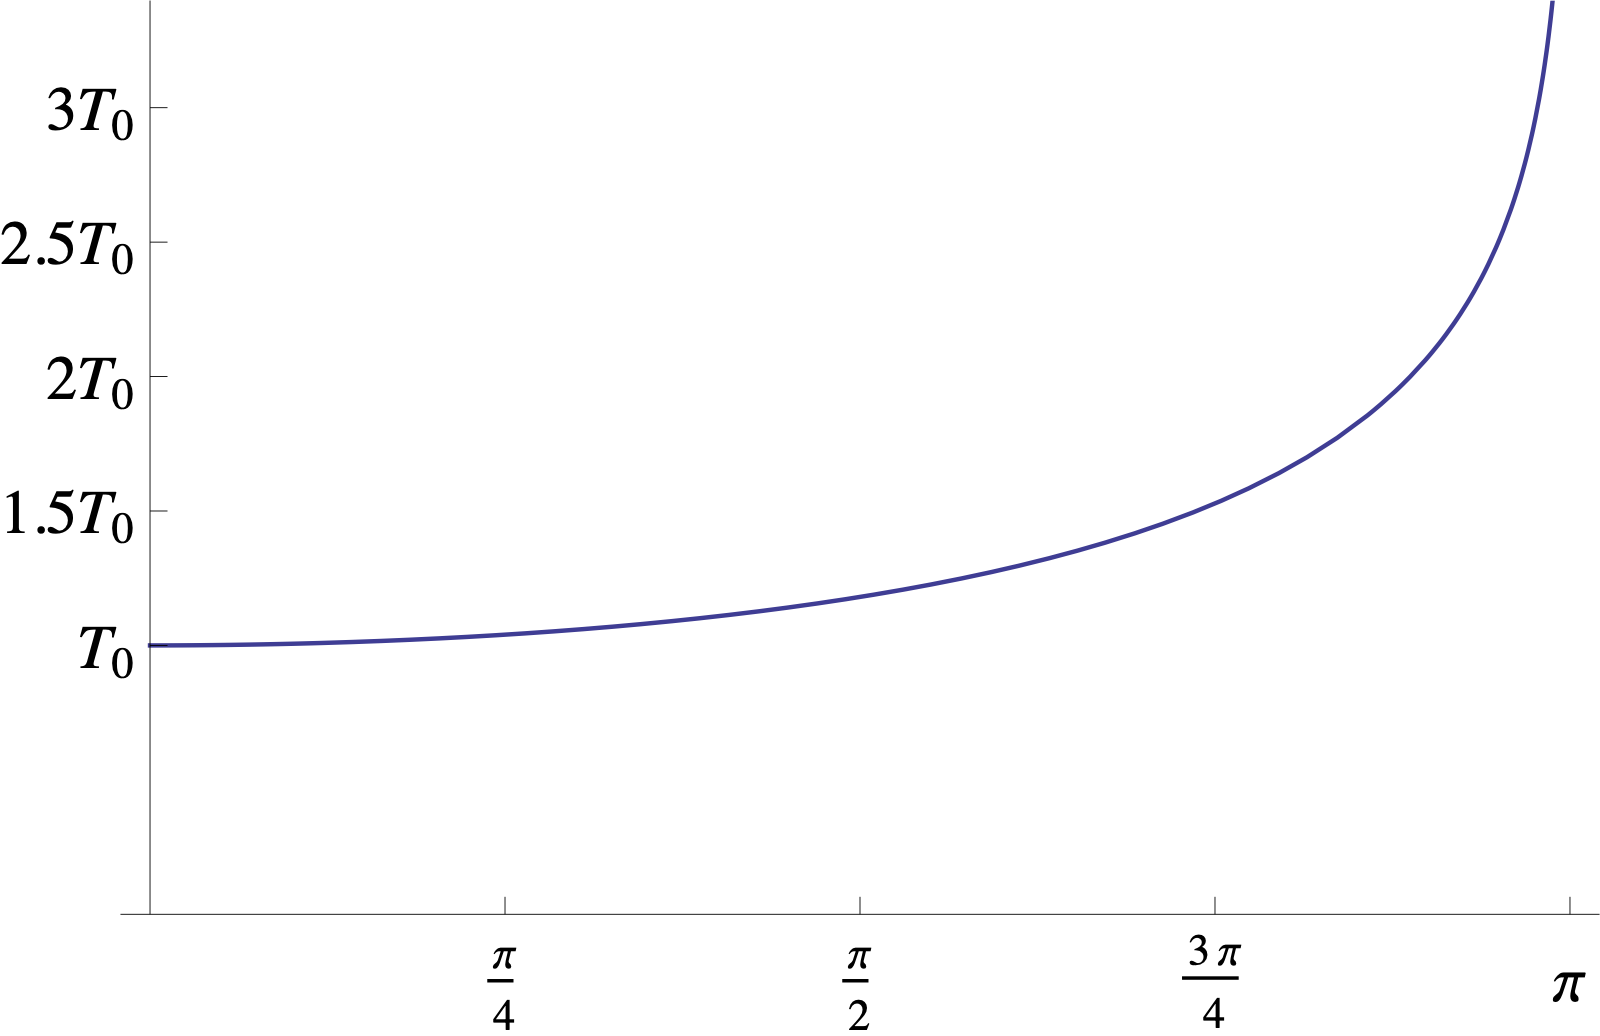
\includegraphics[width=0.70\linewidth]{figures/pendulumperiod.png}\\[0.6em]
{\small Figure 6: The period $T$ of a pendulum (measured in
units of the period $T_0=2\pi\sqrt{\ell/g}$ for small
oscillations) as a function of the oscillation
amplitude $\theta_{\textrm{max}}$.}
\end{center}

\subsection{Falling time of a tree}

A related question concerns the time it takes a
vertical standing object such as a tree to fall over
from its vertical position once it is given a small
destabilizing push. This corresponds almost exactly to
the pendulum starting from the inverted position
$\theta(0)=\pi$, except for the fact that a tree is
actually a \emph{compound} pendulum whose mass is
distributed in some fashion along its entire length.
However, the essential facts remain the same for such
a pendulum --- one simply has to change the length
parameter $\ell$ (see the exercise below, which deals
with the case in which the distribution of mass is
uniform along the length of the rod on which the
pendulum swings). Of course, if the initial angular
velocity $\dot{\theta}(0)$ is $0$, then we have an
equilibrium state and the tree will not fall over. But
this is an unstable equilibrium, so even a tiny
non-zero initial angular velocity
$\dot{\theta}(0)=\omega_0$ would lead to toppling.

To derive the toppling time, which we denote by
$\tau$, observe that the question is equivalent to
asking how long it would take for the pendulum
starting from the modified initial condition
$\theta(0)=0$, $\dot{\theta}(0)=\omega_{\textrm{max}}$
to swing between the angles $\theta=\pi/2$ and
$\theta=\pi$, where $\omega_{\textrm{max}}$, the
angular velocity at the bottom position $\theta=0$
(which is the maximal angular velocity the pendulum
will attain during its motion), is related to
$\omega_0$ by the conservation of energy equation

\begin{align*}
\tfrac12 \omega_0^2 - \lambda \cos(\pi) = \tfrac12 \omega_{\textrm{max}}^2 - \lambda \cos(0),
\end{align*}

\noindent giving the relation
$\omega_{\textrm{max}} = \sqrt{\omega_0^2+4\lambda}$.
In other words, using the solution we just derived for
just such initial conditions, and specifically
\eqref{eq:ellipticintegral-trig}, the quantity we are
trying to compute can be written as the difference of
two times $\tau = t_2-t_1$, where

\begin{align*}
2 \sqrt{\lambda}\, t_1 &= \int_0^{\pi/2} \frac{d\theta}{\sqrt{k^2-\sin^2\tfrac{\theta}{2}}}, \\
2 \sqrt{\lambda}\, t_2 &= \int_0^{\pi} \frac{d\theta}{\sqrt{k^2-\sin^2\tfrac{\theta}{2}}}
\end{align*}

\noindent and
$k=\omega_{\textrm{max}}/2\sqrt{\lambda} =
\sqrt{1+\frac{\omega_0^2}{4\lambda}}$.
This can be written succinctly in terms of the special
function $K(k)$ and another variant, the \emph{incomplete
elliptic integral of the first kind}$F(\alpha, k)$,
defined by

\begin{align*}
F(\alpha,k) = \int_0^\alpha \frac{d\phi}{\sqrt{1-k^2 \sin^2 \phi}}.
\end{align*}

\noindent (Note that $K(k)=F(\pi/2,k)$.) In this notation, we
have

\begin{align*}
\tau &= \frac{1}{2\sqrt{\lambda}} \int_{\pi/2}^\pi \frac{d\theta}{\sqrt{k^2-\sin^2 \tfrac{\theta}{2}}}
= \frac{1}{k \sqrt{\lambda}} \int_{\pi/4}^{\pi/2} \frac{d\phi}{\sqrt{1-k^{-2}\sin^2 \phi}} \\ &=
K(k^{-1}) - F(\pi/4,k^{-1}).
\end{align*}

\noindent Note that $\tau$ becomes arbitrarily large when
$\omega_0$ approaches $0$.

\begin{xexercise}[Compound pendulum]
The falling tree problem is more accurately modeled
by a \emph{compound pendulum}, where we assume the mass $m$
is spread out uniformly along the length of the
swinging rod, instead of being concentrated at its
end. Show that the motion of a compound pendulum with
length $\ell$ is equivalent to that of a simple
pendulum with length $2\ell/3$.
\end{xexercise}

\subsection{The speed of a wave of falling dominoes}

If you have ever set up a long chain of dominoes that
topple each other in a wavelike progression, you must
have wondered how long it would take for all the
dominoes to fall once the experiment is set in motion
(as everyone knows, it ends all too quickly given the
tedious work involved in setting up the dominoes...).
We can now answer this question, in a slightly
simplified model, using the theory of the pendulum
discussed above.\footnote{This section is adapted from the paper \emph{Domino waves}
by C. J. Efthimiou and M. D. Johnson (\emph{SIAM Review}$\textbf{49}$ (2007), 111--120).}

Let us fix some notation for the setup of our domino
wave. We assume a row of standing dominoes of height
$\ell$ is arranged on a plane, with a fixed
horizontal distance of $d$ between each two
successive dominoes. For simplicity, we will model
each domino as a simple inverted pendulum with mass
$m$ (it is not difficult to adapt the analysis to the
case of a compound pendulum) and that its thickness is
small compared to the inter-domino spacing $d$. We
denote by $\beta$ the angle formed between two
adjacent dominoes when one rotates around its contact
point with the floor until it just touches the other;
it is given by

\begin{align*}
\beta = \sin^{-1}\frac{d}{\ell}.
\end{align*}

\noindent See Figure 7.

\begin{center}
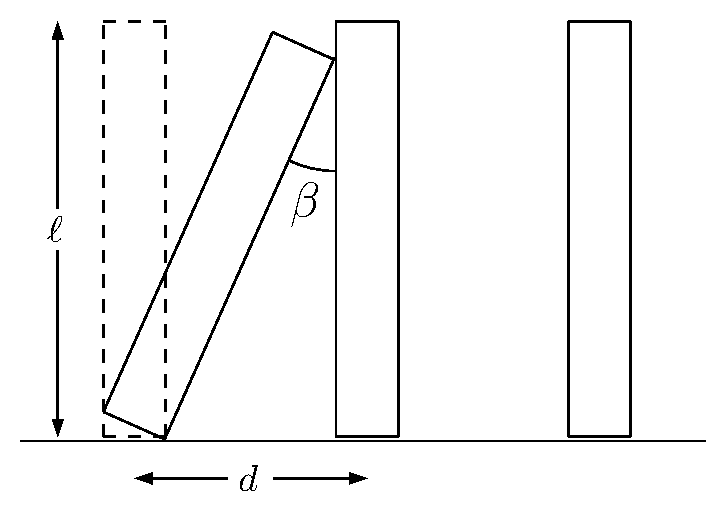
\includegraphics[width=0.60\linewidth]{figures/fallingdominoes.png}\\[0.6em]
{\small Figure 7: A row of falling dominoes.}
\end{center}

\noindent Our analysis of the speed of the domino wave will be
based on analyzing what happens during collisions
between dominoes. We will make the following idealized
assumptions:

\begin{enumerate}[label=(\roman*)]
\item Only collisions between successive dominoes occur
(i.e., we neglect the possible interaction between two
dominoes separated by a third domino).

\item The bottom end of each domino is fixed in place by
static friction with the floor while it topples, so
the domino is only free to rotate around it.

\item Collisions are instantaneous and are elastic, i.e.,
involve no dissipation of energy: both the energy and
momentum of the system are the same \emph{immediately
before and after a collision} (of course, during other
times energy and momentum are not conserved due to
friction forces and dissipation of kinetic energy when
dominoes hit the floor).
\end{enumerate}

\noindent We will now derive equations relating the initial
angular velocity $\omega_0$ of one domino, ``domino
$A$'', to the initial angular velocity $\omega_1$ of
the next one in the row, ``domino $B$''. Two
intermediate quantities that will play a role in the
analysis are the angular velocity $\Omega_0$ of
domino $A$\emph{just before} it collides with domino $B$,
and its angular velocity $\Omega_1$\emph{immediately
after} the collision. The relationships between the
four quantities
$\omega_0, \omega_1, \Omega_0, \Omega_1$ are
determined by the conservation of energy and momentum.

First, conservation of energy during the motion of
domino $A$ from the time it starts to rotate until it
hits domino $B$ gives the equation

\begin{align*}
\tfrac12 m \ell^2 \omega_0^2 + mg\ell = \tfrac12 m \ell^2 \Omega_0^2 + mg\ell \cos \beta,
\end{align*}

\noindent which can be solved for $\Omega_0$ to give

\begin{equation*} \tag{25}\label{eq:dominowave-cons1}
\begin{split}
\Omega_0^2 = \omega_0^2 + \frac{2g}{\ell}(1-\cos \beta).
\end{split}
\end{equation*}

\noindent Next, conservation of energy during the collision
gives

\begin{align*}
\tfrac12 m\ell^2 \Omega_0^2 = \tfrac12 m\ell^2 \Omega_1^2 + \tfrac12m\ell^2 \omega_1^2,
\end{align*}

\noindent which simplifies to

\begin{equation*} \tag{26}\label{eq:dominowave-cons2}
\begin{split}
\Omega_0^2 = \Omega_1^2 + \omega_1^2.
\end{split}
\end{equation*}

\noindent To express the conservation of momentum, it is easier
(and equivalent) to write an equation for the
conservation of \emph{angular} momentum around the base
point of domino $B$. This gives

\begin{align*}
m\ell^2\Omega_0 \cos^2\beta = m\ell^2\Omega_1 \cos^2 \beta + m\ell^2\omega_1.
\end{align*}

\noindent That is,

\begin{equation*} \tag{27}\label{eq:dominowave-cons3}
\begin{split}
\Omega_0\cos^2\beta = \Omega_1\cos^2\beta + \omega_1.
\end{split}
\end{equation*}

\noindent It is not difficult to solve \eqref{eq:dominowave-cons2},
\eqref{eq:dominowave-cons3} for $\Omega_1$ and $\omega_1$,
to get

\begin{equation*} \tag{28}\label{eq:dominowave-cons4}
\begin{split}
\omega_1 &= f_+ \Omega_0, \\
\Omega_1 &= \frac{f_+}{f_-} \Omega_0,
\end{split}
\end{equation*}

\noindent where

\begin{align*}
f_{\pm} = \frac{2}{\cos^2 \beta \pm \cos^{-2}\beta}.
\end{align*}

\noindent Plugging the value of $\Omega_0$ obtained from
\eqref{eq:dominowave-cons1} into \eqref{eq:dominowave-cons4}
finally yields an equation expressing $\omega_1$ in
terms of $\omega_0$, namely

\begin{align*}
\omega_1 = f_+ \sqrt{\omega_0^2 + \frac{2g}{\ell}(1-\cos \beta)} = H(\omega_0).
\end{align*}

\noindent Our analysis has produced the following result: if we
start the domino wave going by giving the first domino
in the chain a slight push that gives it an initial
angular velocity $\omega_0$, then the next domino it
will collide with will start its motion with an
initial angular velocity equal to
$\omega_1=H(\omega_0)$. That domino will collide with
a third domino, which will acquire an initial angular
velocity of $\omega_2=H(\omega_1)=H(H(\omega_0))$,
and so forth: the $n$th domino in the chain will get
an initial angular velocity of

\begin{align*}
\omega_{n-1} = H^{n}(\omega_0) = H(H(H(\ldots H(\omega_0)))\ldots)
\end{align*}

\noindent (the $n$th functional iterate of $H$). While it may
appear as if the way the wave gets started is
important, a more careful look at the properties of
the function $H$ shows that in fact the wave will
settle down to an equilibrium state in which each
domino gets an initial angular velocity equal to

\[
\omega_\infty = \lim_{n\to\infty} \omega_n.
\]

\noindent This equilibrium angular velocity must satisfy the
equation

\begin{align*}
\omega_\infty = H(\omega_\infty) = f_+ \sqrt{\omega_0^2 + \frac{2g}{\ell}(1-\cos \beta)},
\end{align*}

\noindent which can be solved to give

\begin{align*}
\omega_\infty = \frac{2g}{\ell}\frac{f_+^2}{1-f_+^2}(1-\cos\beta) = \frac{2g}{\ell}f_-^2(1-\cos\beta).
\end{align*}

\noindent We are finally ready to answer the original question
regarding the speed of a traveling domino wave. Once
the wave has reached its equilibrium state, each
domino starts its motion with the angular velocity
$\omega_\infty$, and rotates through an angle of
$\beta$ before colliding with the next domino. By the
theory of falling times for the inverted pendulum
discussed in the previous section, the time this
rotation takes is given by

\begin{align*}
\tau &= \frac{1}{2\sqrt{g/\ell}} \int_{\pi-\beta}^{\pi} \frac{d\theta}{\sqrt{k^2-\sin^2\tfrac{\theta}{2}}}
= \frac{1}{k\sqrt{g/\ell}} \int_{(\pi-\beta)/2}^{\pi/2} \frac{d\phi}{\sqrt{1-k^{-2}\sin^2 \phi}} \\
&= \frac{1}{k\sqrt{g/\ell}} \left( K(k^{-1})-F((\pi-\beta)/2,k^{-1}) \right),
\end{align*}

\noindent where

\begin{align*}
k = \sqrt{\frac{4g/\ell+\omega_\infty^2}{4g/\ell}}.
\end{align*}

\noindent During each such rotation cycle, one can say that the
wave has travelled the distance $d$ equal to the
inter-domino spacing. Thus, the speed of the domino
wave is given by the grand formula

\begin{align*}
v_{\textrm{wave}} = \frac{d}{\tau} = k d \sqrt{\frac{g}{\ell}}
\left( K(k^{-1})-F((\pi-\beta)/2,k^{-1}) \right)^{-1},
\end{align*}

\noindent Note that all quantities in this formula are
expressed as functions of the ``free'' parameters
$d, \ell$ and $g$.

\chapter{Part 2 — Discrete-time dynamics, chaos and ergodic theory}

\section{Introduction}
\label{sec:ergodic-intro}

In this part of the course, we will consider a
different flavor of nonlinear systems in which time
flows in discrete steps instead of continuously. The
set of states of such a system is a set $\Omega$
commonly referred to as the \emph{state space}. In many
cases $\Omega$ is a subset of $\mathbb{R}$ or the
vector space $\mathbb{R}^d$. The state of the system
as a function of time is a sequence
$(x_n)_{n=0}^\infty$ of elements of $\Omega$; i.e.,
it can be thought of as a function of time
$n\mapsto x_n$, where the time variable takes only
discrete values (and therefore is frequently denoted
by the letter $n$ instead of $t$).

With a continuous-time system, we commonly use an
ordinary differential equation $\dot{x}=F(x,t)$ to
describe the \emph{dynamics}, i.e., the rules according to
which the state of the system evolves. The analogous
concept for a discrete-time system $(x_n)_{n\ge 0}$
is called a \emph{difference equation}, which is an
equation of the form

\begin{equation*} \tag{29}\label{eq:differenceeq}
\begin{split}
x_{n+1}-x_n &= F(x_n, n),
\end{split}
\end{equation*}

\noindent where $F$ is a function
$F:\Omega\times \mathbb{N}_0\to\Omega$ (note that
this only makes sense if the set $\Omega$ is a subset
of a vector space so that the operation of subtraction
is defined). Given a state $a \in \Omega$, we can
solve the difference equation \eqref{eq:differenceeq}
starting from the initial condition $x_0=a$. The
solution is obtained (and is easily seen to be unique)
by rewriting \eqref{eq:differenceeq} as
$x_{n+1}=x_n+F(x_n,n)$ and iterating this ``forward
evolution'' rule, e.g.,

\begin{align*}
x_1 &= x_0 + F(x_0,0), \\ x_2&= x_1+F(x_1,1), \\ x_3&=x_2+F(x_2,2), \ldots
\end{align*}

\noindent You can see that this process of iteration is much
more straightforward than the process of solving ODEs.
For example, one does not have to deal with issues of
existence or uniqueness of solutions. In fact, in many
cases one does not even need to know calculus to work
with such equations. On the other hand, as we shall
see, many of the other delicate issues that show up in
the study of ODEs (such as chaotic behavior, stability
and instability, and bifurcations) exist also for
difference equations.

\section{Difference equations and maps}

As we commented above, the equation
\eqref{eq:differenceeq} can be rewritten in a way that
eliminates the differencing operation, namely as

\begin{equation*} \tag{30}\label{eq:differenceeq-map}
\begin{split}
x_{n+1} &= T(x_n,n),
\end{split}
\end{equation*}

\noindent where $T(x_n,n)=x_n+F(x_n,n)$. In many cases the
evolution rule of a system is described by giving the
function $T:\Omega\times \mathbb{N}_0\to\Omega$
instead of $F:\Omega\times \mathbb{N}_0\to\Omega$;
clearly these two descriptions are equivalent, but the
latter has the advantage that it makes sense even when
$\Omega$ is an abstract set with no extra structure
(in which case there is no ``differencing'' operation,
so it does not make sense to talk about a difference
equation). In the case of the equation
\eqref{eq:differenceeq-map}, usually it will be called a
\emph{recurrence relation} instead of a difference
equation. An especially nice (and very common)
situation is one in which $T$ does not depend on the
time variable $n$, but instead is simply a function
$T(x)$ of the state. In this case
\eqref{eq:differenceeq-map} becomes

\begin{align*}
x_{n+1} &= T(x_n),
\end{align*}

\noindent and the function $T:\Omega\to\Omega$ is called the
\emph{evolution map}, or just the \emph{map}, associated with
the system; it tells the state of the system one unit
of time into the future as a function of the present
state. We shall be concerned exclusively with such
time-independent systems.

\begin{example}[Arithmetic growth]
The equation for arithmetic growth is

\begin{align*}
x_{n+1} = x_n + b,
\end{align*}

\noindent where $b\in\mathbb{R}$ is a constant. As a difference
equation, it will be written as

\begin{align*}
x_{n+1}-x_n = b.
\end{align*}

\noindent Its solution is the arithmetic sequence

\[
x_n = x_0 + bn.
\]

\end{example}

\begin{example}[Geometric growth]
The equation for geometric growth is

\begin{align*}
x_{n+1} = r x_n ,
\end{align*}

\noindent where $r\in\mathbb{R}$ is a constant, or
$x_{n+1}-x_n = (r-1)x_n$ as a difference equation
(so, like the ODE $\dot{x}(t)=cx(t)$, it is suitable
to model situations in which the rate of change of a
quantity is proportional to it). The solution is the
geometric sequence

\[
x_n = x_0 r^n.
\]

\end{example}

\begin{example}[Fibonacci numbers]
The sequence of Fibonacci numbers $(F_n)_{n=1}^\infty$
is defined as the unique sequence that satisfies the
initial conditions $F_1=F_2=1$ together with the
recurrence relation

\begin{equation*} \tag{31}\label{eq:recurrence-fibonacci}
\begin{split}
F_{n+2}=F_{n+1}+F_n \qquad (n\ge0).
\end{split}
\end{equation*}

\noindent Note that this is a \emph{second-order recurrence
relation} --- the discrete-time analogue of a second
order differential equation. In general, a
second-order recurrence will have the form

\begin{align*}
x_{n+2} &= T(x_n,x_{n+1},n),
\end{align*}

\noindent i.e., each successive value in the sequence is
computed as a function of the last two values (and
possibly the time parameter). To solve the recurrence
we will need to specify not one but two initial
conditions, e.g. (if we are trying to solve the
recurrence for $n\ge0$) $x_0$ and $x_1$.

It is well-known that the solution to the recurrence
\eqref{eq:recurrence-fibonacci} is given by the amusing
formula

\begin{equation*} \tag{32}\label{eq:fibonacci-closedform}
\begin{split}
F_n = \frac{1}{\sqrt{5}}\left(\frac{1+\sqrt{5}}{2}\right)^n-\frac{1}{\sqrt{5}}\left(\frac{1-\sqrt{5}}{2}\right)^n.
\end{split}
\end{equation*}

\noindent This can be proved by induction by verifying the
initial conditions and then substituting the
expression on the right-hand side into
\eqref{eq:recurrence-fibonacci}.

Is there a systematic way to derive such mysterious
formulas? As with ODEs, it is often more convenient to
represent a second- (or higher-) order system as a
first-order system. We can do this by constructing a
new system whose state space is $\mathbb{R}^2$
instead of $\mathbb{R}$, where the recurrence
relation is given by

\begin{equation*} \tag{33}\label{eq:recurrence-fib-matrix}
\begin{split}
\left( \begin{array}{c}X_{n+1}\\Y_{n+1}\end{array}\right) =
\left( \begin{array}{c} X_n+Y_n \\ X_n
\end{array}\right) =
\left( \begin{array}{cc}
1&1\\1&0
\end{array}\right)
\left( \begin{array}{c}X_n\\Y_n\end{array}\right).
\end{split}
\end{equation*}

\noindent Substituting
$\left(
\begin{array}{c}X_n\\Y_n\end{array}\right)=\left(
\begin{array}{c}F_{n+1}\\F_n\end{array}\right)$
into \eqref{eq:recurrence-fib-matrix}, we get

\begin{align*}
\left( \begin{array}{c}F_{n+2}\\F_{n+1}\end{array}\right)
=
\left( \begin{array}{c} X_{n+1}\\ Y_{n+1}
\end{array}\right) =
\left( \begin{array}{c} X_n+Y_n \\ X_n
\end{array}\right) =
\left( \begin{array}{c} F_{n+1}+F_n \\ F_{n+1}
\end{array}\right),
\end{align*}

\noindent which reproduces \eqref{eq:recurrence-fibonacci}.
Denoting the $2\times 2$ matrix on the right-hand
side of \eqref{eq:recurrence-fib-matrix} by $A$, the
recurrence relation \eqref{eq:recurrence-fib-matrix} can
be thought of as ``geometric growth with a matrix
multiplier''. By analogy with the geometric growth
example, it is easy to see that its solution is

\begin{equation*} \tag{34}\label{eq:fibonacci-matrixsol}
\begin{split}
\left(\begin{array}{c}
F_{n+1}\\F_n
\end{array}\right) = A^{n-1}
\left(\begin{array}{c}
1\\1
\end{array}\right).
\end{split}
\end{equation*}

\noindent The formula \eqref{eq:fibonacci-closedform} can now be
derived using standard diagonalization techniques from
linear algebra.
\end{example}

\begin{xexercise}
Derive the formula \eqref{eq:fibonacci-closedform} by
diagonalizing the matrix
$A=\left(\begin{array}{cc}
1&1\\0&1\end{array}\right)$
and using the solution \eqref{eq:fibonacci-matrixsol}.
\end{xexercise}

\begin{example}[$3x+1$ map]
On the state space $\Omega=\mathbb{N}$, define the
map $T:\mathbb{N}\to\mathbb{N}$ by

\begin{align*}
T(x) &= \begin{cases} x/2 & \textrm{if $x$ is even}, \\ 3x+1 & \textrm{if $x$ is odd}.
\end{cases}
\end{align*}

\noindent It is interesting to ask what happens if we start
from some initial value $x_0$ and apply the map to
get the subsequent values
$x_1=T(x_0), x_2=T(x_1)=T(T(x_0)),$ etc. Let's look
at some examples:

\begin{align*}
x=1: \quad & 1\mapsto 4 \mapsto 2 \mapsto 1 \mapsto [\textrm{infinite cycle of }4,2,1], \\
x=3: \quad & 3\mapsto 10\mapsto 5\mapsto 16\mapsto 8 \mapsto 4 \mapsto2\mapsto 1 \mapsto
[\textrm{cycle of }4,2,1], \\
x=6: \quad & 6 \mapsto 3 \mapsto \ldots[\textrm{see above}] \ldots \mapsto [\textrm{infinite cycle of }4,2,1], \\
x=7: \quad & 7 \mapsto 22\mapsto 11\mapsto 34\mapsto 17\mapsto 52\mapsto 26\mapsto13\mapsto40
\mapsto20 \\ & \ \,\mapsto10\mapsto \ldots[\textrm{see above}] \ldots \mapsto [\textrm{infinite cycle of }4,2,1].
\end{align*}

\noindent Is it true that for any initial number $x_0$,
iterating the map will eventually reach the infinite
cycle $4,2,1$? This famous question, known as the
\emph{Collatz problem}, was proposed 75 years ago.
Extensive research and numerical computations suggest
that the answer is yes, but no one knows how to prove
this.
\end{example}

\begin{example}[Discretized forward evolution of an ODE]
If $\dot{x}=F(x)$ is an autonomous ODE (say on
$\mathbb{R}$ or some region of $\mathbb{R}^d$), we
can discretize time by allowing it to flow only in
integer multiples of some fixed time step $\tau$.
That is, we consider the phase flow
$(\varphi_t)_{t\ge 0}$ of the system, and for each
initial condition $x_0$ define a sequence
$(x_n)_{n=0}^\infty$ by

\[
x_n = \varphi_{n\tau}(x_0) \qquad (n\ge 1).
\]

\noindent Because the phase flow satisfies the equation
$\varphi_{t+s}(x)=\varphi_t\circ \varphi_s(x)$, it is
easy to see that $x_n$ satisfies the recurrence
relation

\[
x_{n+1} = T(x_n),
\]

\noindent where $T = \varphi_\tau$. So, the ODE has given rise
to a discrete-time dynamical system by fixing the
time-step $\tau$.
\end{example}

\begin{example}[Poincaré section map of an ODE]
The time-discretization procedure described in the
above example requires an arbitrary choice of a time
unit. There is a more natural way to construct a
discrete-time dynamical system starting from an ODE
that avoids this difficulty, called the \emph{Poincaré
section map} or \emph{first-return map}. Assume the phase
space $\Omega$ of the ODE is $n$-dimensional (i.e., a
subset of $\mathbb{R}^n$, or more generally, an
``$n$-dimensional manifold''). Furthermore, assume
that there is an $(n-1)$-dimensional subset
$A \subset \Omega$ that has the property that all
solutions are known to pass infinitely many times
through $A$ and through its complement
$\Omega\setminus A$. The Poincaré map $T:A\to A$ is
defined by

\begin{align*}
T(x) = \varphi_{\tau(x)}(x),
\end{align*}

\noindent where $\tau(x) = \inf\{ t>0\,:\, \varphi_t(x)\in A\}$
and $\varphi_t:\Omega\to\Omega$ is the phase flow of
the system.

Poincaré maps are an extremely useful tool in the
analysis of ODEs. A nice illustration of this general
construction and its applicability in a specific
example is given on page 279 of Strogatz's book
\emph{Nonlinear Dynamics and Chaos}.
\end{example}

\begin{example}[Logistic map]
An important and fascinating example that we will
spend a lot of time discussing is the \emph{logistic map}$L:[0,1]\to[0,1]$, a dynamical system with state
space $\Omega=[0,1]$. It is actually not one map, but
a family of maps $L=L_r$ where $0\le r\le 4$ is a
parameter. The map $L_r$ is defined by the formula

\begin{align*}
L_r(x) = rx(1-x).
\end{align*}

\noindent The logistic map was introduced as a simple model for
the fluctuations in the population of a species of
animals (or plants, or bacteria etc.) in an
environment with limited resources. The idea is that
$x$ represents the size of the population (as a
fraction of some absolute maximum), and the
assumptions are that for small values of $x$, the
population will increase in a roughly geometric
pattern, but for large values of $x$ the growth will
taper off as the animals deplete the available food
resources, leading to starvation and a dramatic
reduction in population size for even larger values of
$x$ (see Figure 8).

\begin{center}
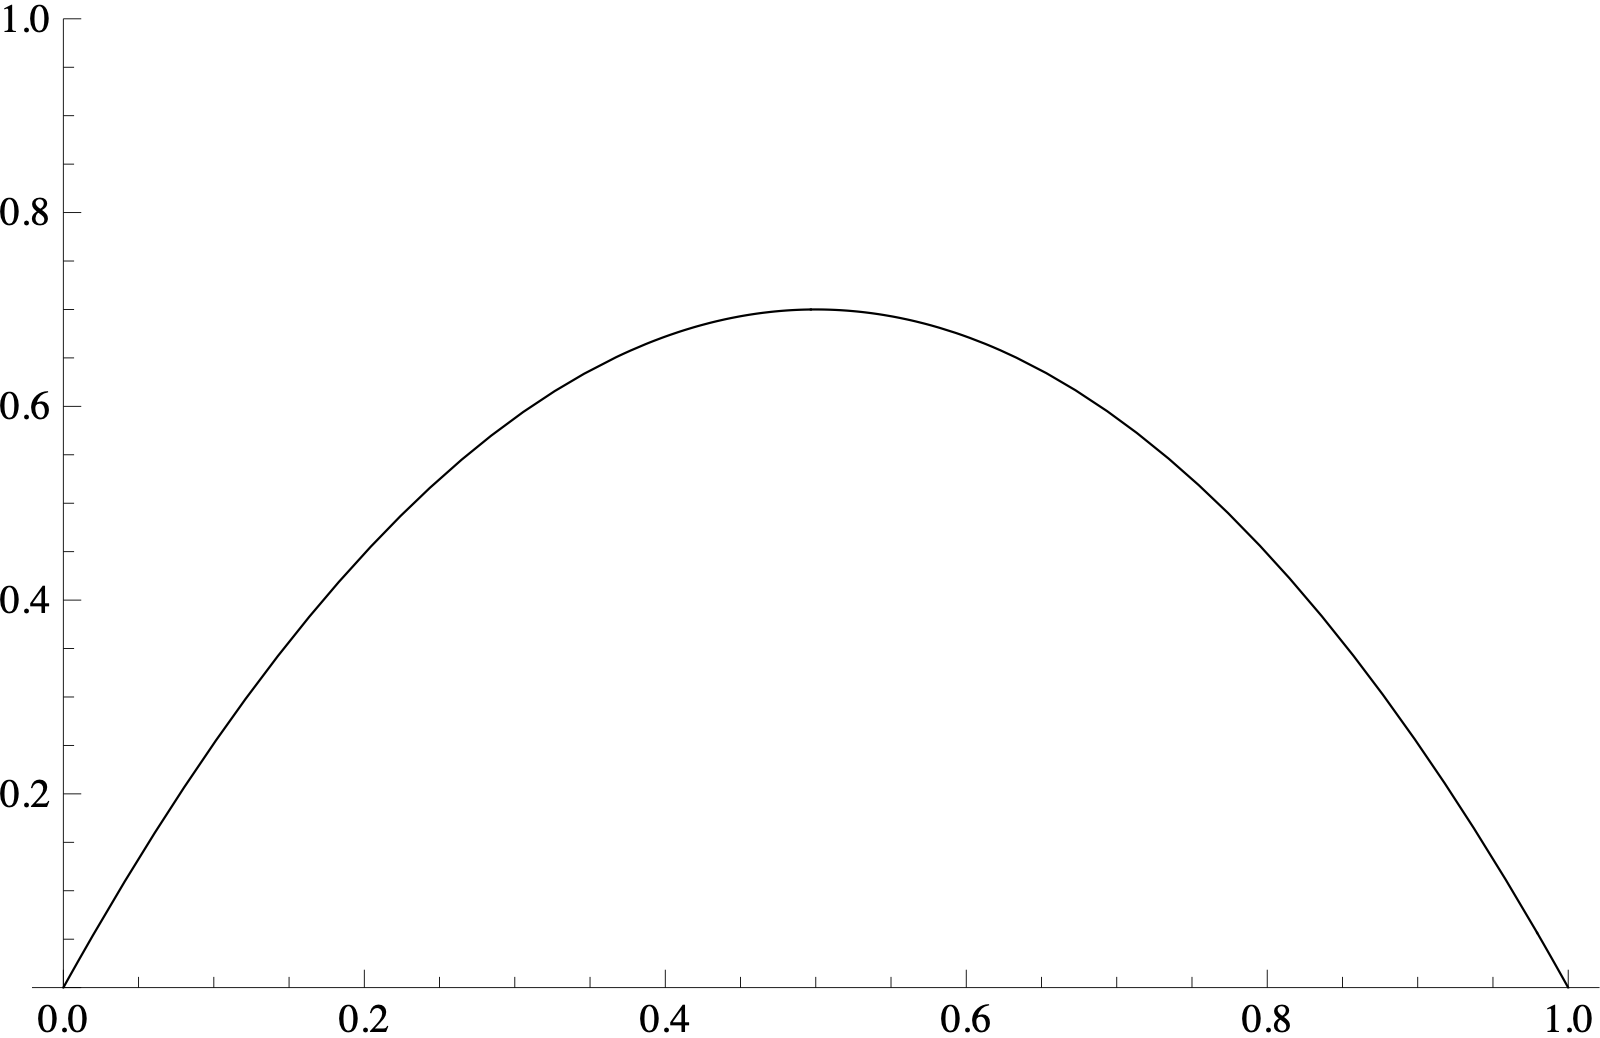
\includegraphics[width=0.62\linewidth]{figures/logisticmap28.png}\\[0.6em]
{\small Figure 8: The logistic map $L_r$ for $r=2.5$.}
\end{center}

\noindent The behavior of the logistic map, depending on the
value of $r$, can be very simple, or very complicated
(or somewhere in between) --- in fact, it is one of
the simplest examples of a chaotic system, and
studying it will give us valuable insights into the
more general theory of discrete-time dynamical
systems.
\end{example}

\begin{example}[Billiard maps]
An interesting class of examples with a geometric
flavor are the billiard maps. Given some odd-shaped
bounded region $D$ in the plane, we let a billiard
ball bounce around in $D$, reflecting off the walls
without loss of energy. This is a continuous time
system, but a standard simplification step is to take
its Poincaré section map with respect to the set of
times at which the ball hits the wall. Thus, the state
space of a billiard system considered as a
discrete-time system is the set of pairs $(x,\theta)$
where $x \in \partial D$ is a boundary point and
$\theta\in [0,2\pi)$ is the angle of the ball's
velocity immediately after it reflects off the wall at
$x$.

Billiard systems exhibit an extremely rich behavior
that is extensively studied by mathematicians and
physicists as a toy model for more complicated systems
such as the behavior of an ideal gas. Depending on the
shape of the ``billiard table,'' the system can have a
chaotic structure or a more orderly behavior where
nearby initial conditions do not drift far apart. See
Figure 9 for some examples.

\begin{center}
\begin{minipage}[t]{0.44\linewidth}\centering
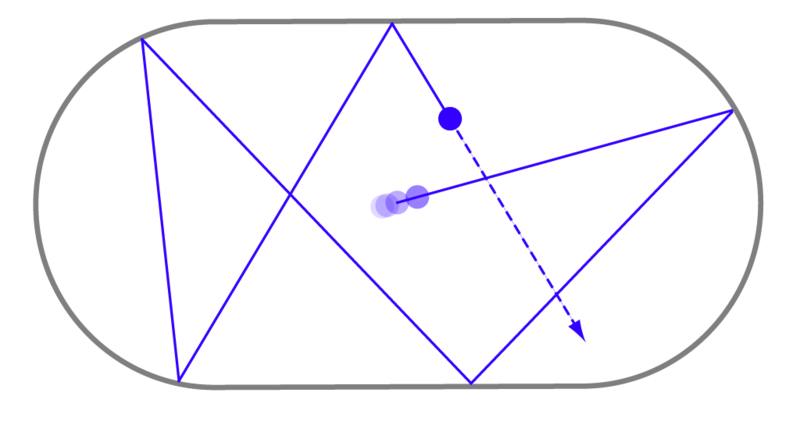
\includegraphics[width=\linewidth]{figures/billiards-bunimovichstadium.png}\\
(a)
\end{minipage}\hspace{0.02\linewidth}%
\begin{minipage}[t]{0.44\linewidth}\centering
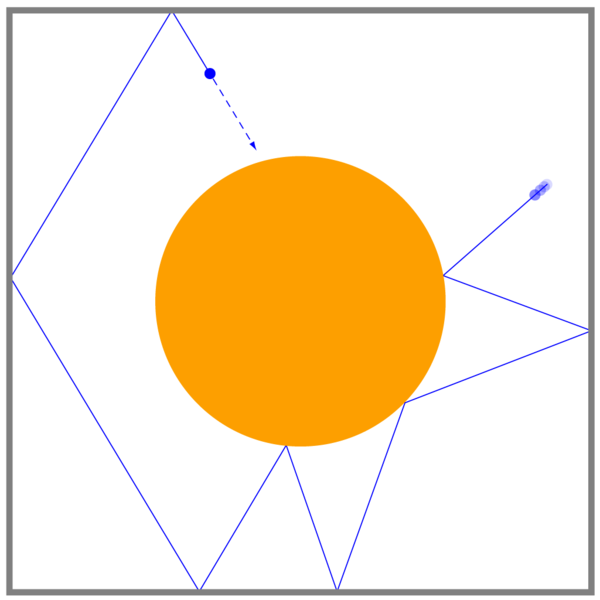
\includegraphics[width=\linewidth]{figures/billiards-sinai.png}\\
(b)
\end{minipage}\hspace{0.02\linewidth}%
\begin{minipage}[t]{0.44\linewidth}\centering
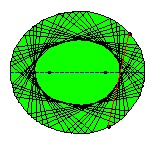
\includegraphics[width=\linewidth]{figures/billiard-ellipse.jpg}\\
(c)
\end{minipage}\hspace{0.02\linewidth}%
\begin{minipage}[t]{0.44\linewidth}\centering
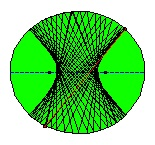
\includegraphics[width=\linewidth]{figures/billiard-hyperbola.jpg}\\
(d)
\end{minipage}\\[0.6em]
{\small Figure 9: Billiard dynamical systems: (a) The
``Bunimovich stadium''; (b) The ``Sinai billiard''
(source: Wikipedia); (c) and (d) billiard in an
ellipse-shaped region.}
\end{center}

\end{example}

\section{Interval maps}

A discrete-time system is called \emph{one-dimensional} if
it has either $\mathbb{R}$ or a sub-interval of
$\mathbb{R}$ as its state space. There are many
interesting examples of such systems, and it will be
especially convenient to focus on maps defined on an
interval, usually taken to be the unit interval
$[0,1]$ (or in some cases the open interval $(0,1)$).
Such a map is called an \emph{interval map}. The logistic
map is one especially interesting example of an
interval map. Here are some additional maps that we
will consider later.

\begin{example}[Doubling map]
The doubling map $D:[0,1)\to[0,1)$ is defined by

\begin{align*}
D(x) &= 2x \textrm{ mod } 1 = \begin{cases}
2x & \textrm{if }0\le x<\tfrac12, \\ 2x-1 & \textrm{if }\tfrac12 \le x < 1,
\end{cases}
\end{align*}

\noindent (see Figure 10). As we will see later, it is closely
related to binary expansions of real numbers in
$(0,1)$. In particular, trying to understand the
statistical properties of binary expansions of random
numbers leads naturally to questions about properties
of the doubling map --- see Section
\ref{sec:normalnumbers} for further discussion.
\end{example}

\begin{example}[Circle rotation map]
For $0<\alpha<1$, the circle rotation map
$R_\alpha:[0,1)\to[0,1)$ is defined by

\begin{align*}
R_\alpha(x) = x+\alpha\textrm{ mod }1
= \begin{cases}
x+\alpha & \textrm{if }0\le x<1-\alpha, \\
x+\alpha-1 & \textrm{if } 1-\alpha \le x\le 1.
\end{cases}
\end{align*}

\noindent The reason for the name of this map is that if one
considers the interval $[0,1]$ as a topological
circle by identifying the two ends, the map
corresponds to a rotation of the circle by the angle
$2\pi \alpha$.
\end{example}

\begin{example}[Tent map]
The tent maps are another one-parameter family of
maps $\Lambda_a$, $0<a\le 2$, defined by

\begin{align*}
\Lambda_a(x) &= \begin{cases}
ax & \textrm{if }0\le x<\tfrac12, \\ a-ax & \textrm{if }\tfrac12 \le x \le 1.
\end{cases}
\end{align*}

\noindent Figure 10 illustrates the extreme case $a=2$.
\end{example}

\begin{example}[Gauss map]
Denote by $\{ x \}=x-\lfloor x\rfloor$ the fractional
part of a real number $x$ (where
$\lfloor x\rfloor = \max\{ n\in\mathbb{Z}\,:\,n\le
x\}$
is the integer part of $x$). The Gauss map
$G:(0,1)\to[0,1)$, which is related to so-called
continued fraction expansions of real numbers, is
defined by

\begin{align*}
G(x) &= \left\{ \frac{1}{x} \right\},
\end{align*}

\noindent i.e., $G(x)=1/x-n$ for $1/(n+1)<x<1/n$,
($n=1,2,\ldots$).
\end{example}

\begin{xexercise}[Properties of the Gauss map]

\begin{enumerate}[label=\arabic*.]
\item Show (or read in a number theory textbook how to
show) that the numbers $x\in [0,1]$ for which the
sequence of iterates $G^n(x)$ eventually reaches $0$
(and is therefore undefined for larger values of $n$)
are precisely the rational numbers.

\item Show that the eventually periodic points of $G$
(numbers $x$ for which for some $n$, $G^n(x)$ belongs
to an $m$-cycle, see the definition below) are the
quadratic irrationals, i.e., the irrational numbers
which are solutions of quadratic equations.

\item Find a formula for all the fixed points of $G$.
\end{enumerate}

\end{xexercise}

\begin{center}
\begin{minipage}[t]{0.44\linewidth}\centering
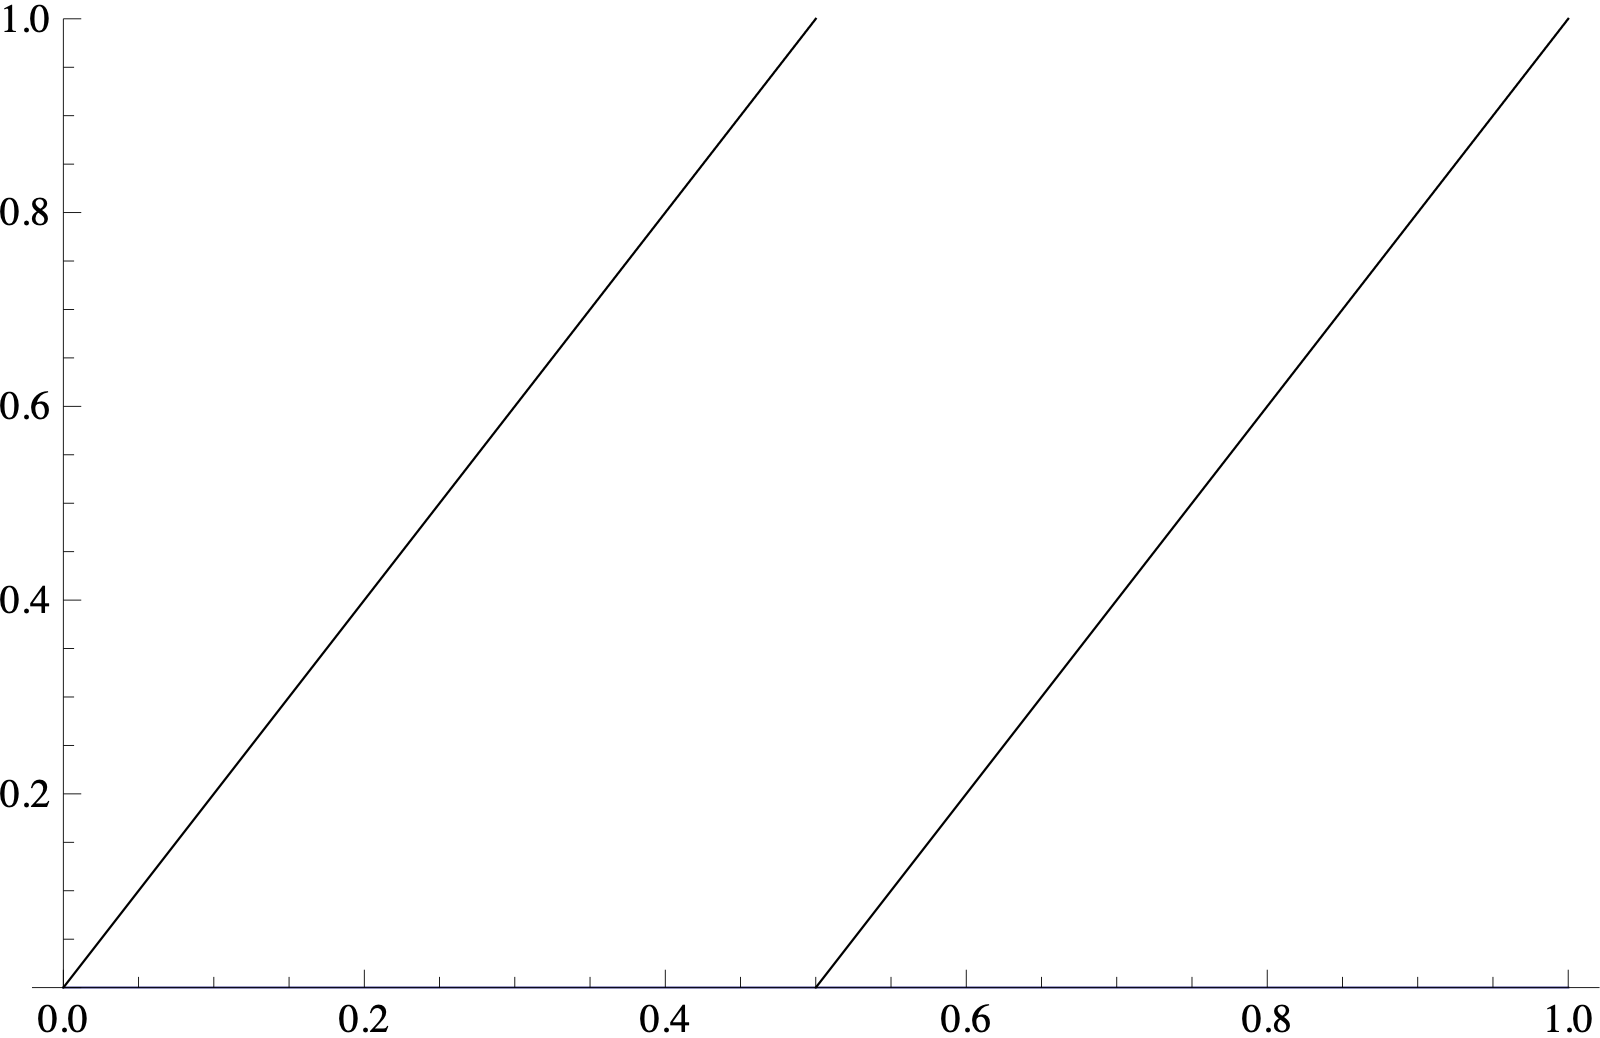
\includegraphics[width=\linewidth]{figures/doublingmap.png}\\
(a)
\end{minipage}\hspace{0.02\linewidth}%
\begin{minipage}[t]{0.44\linewidth}\centering
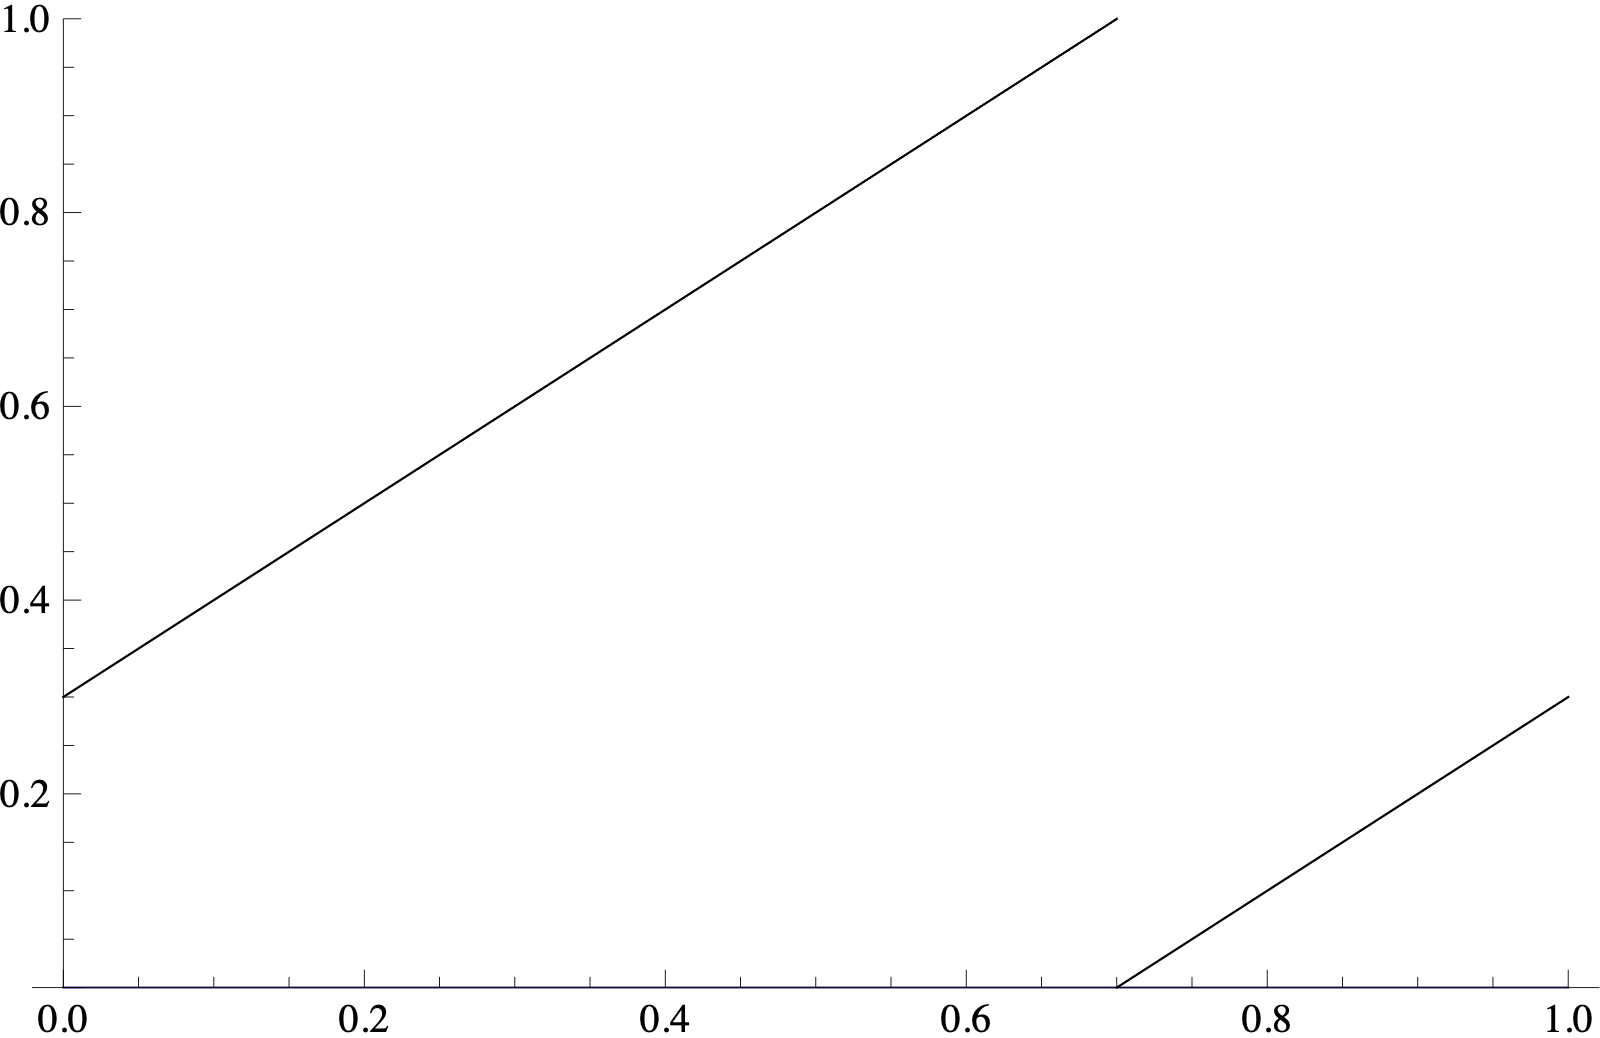
\includegraphics[width=\linewidth]{figures/circlerotation03.png}\\
(b)
\end{minipage}\hspace{0.02\linewidth}%
\begin{minipage}[t]{0.44\linewidth}\centering
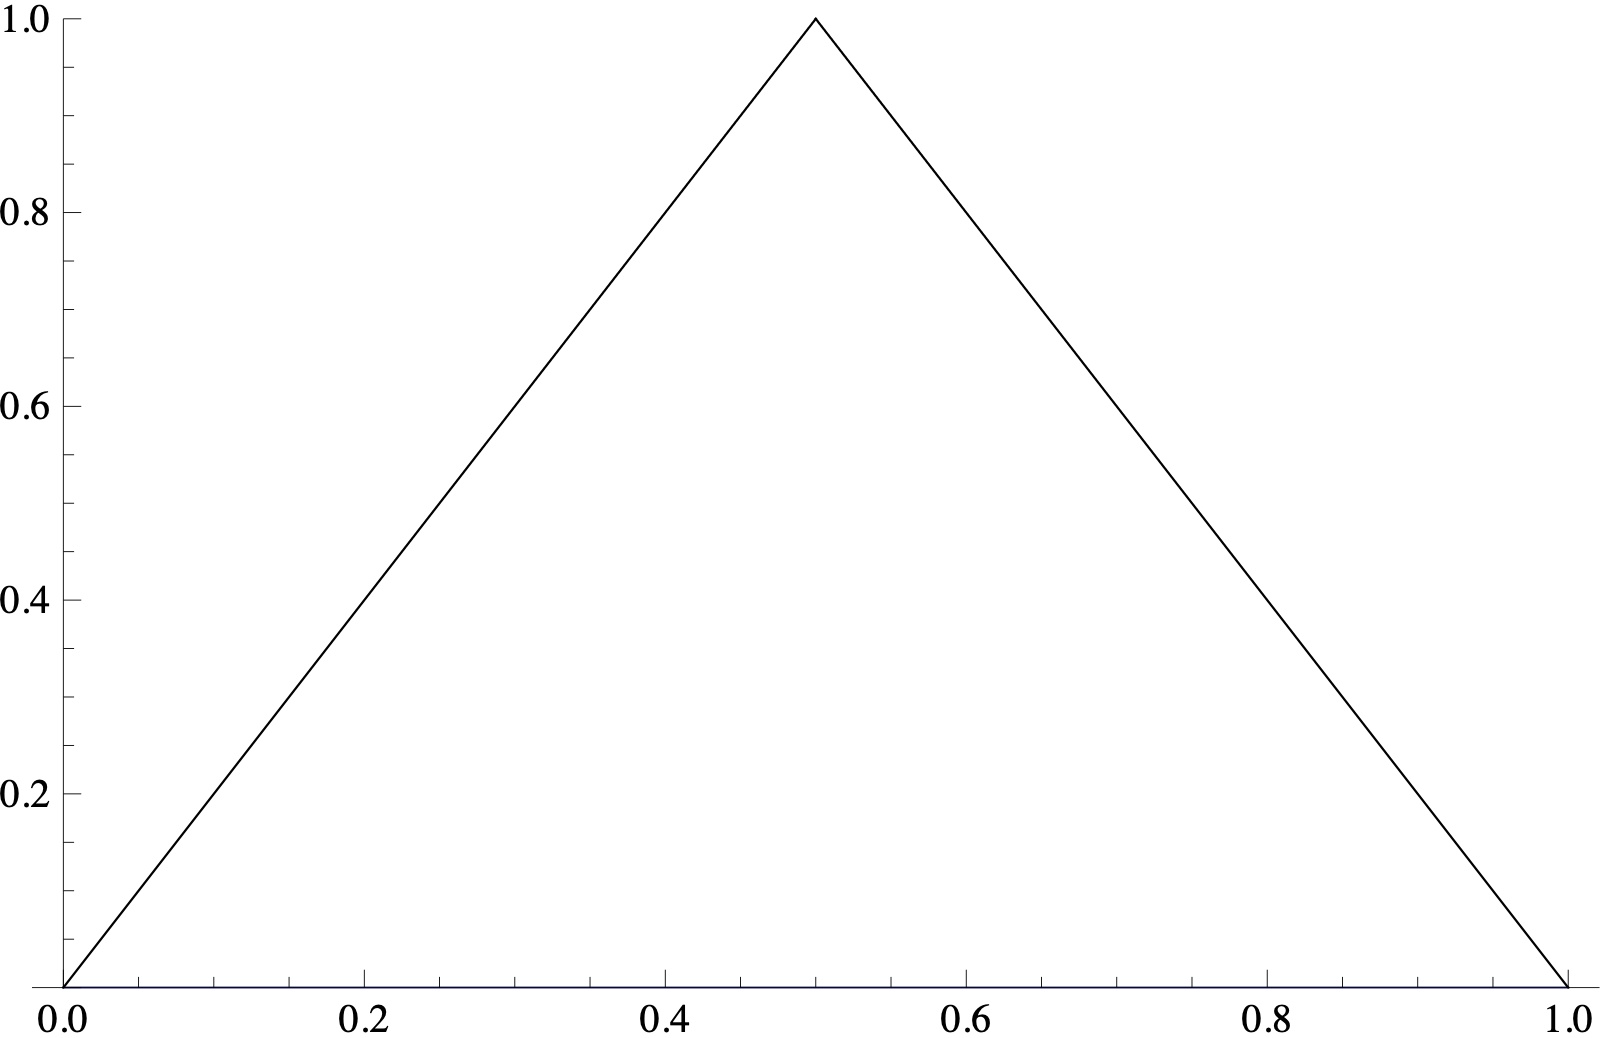
\includegraphics[width=\linewidth]{figures/tentmap.png}\\
(c)
\end{minipage}\hspace{0.02\linewidth}%
\begin{minipage}[t]{0.44\linewidth}\centering
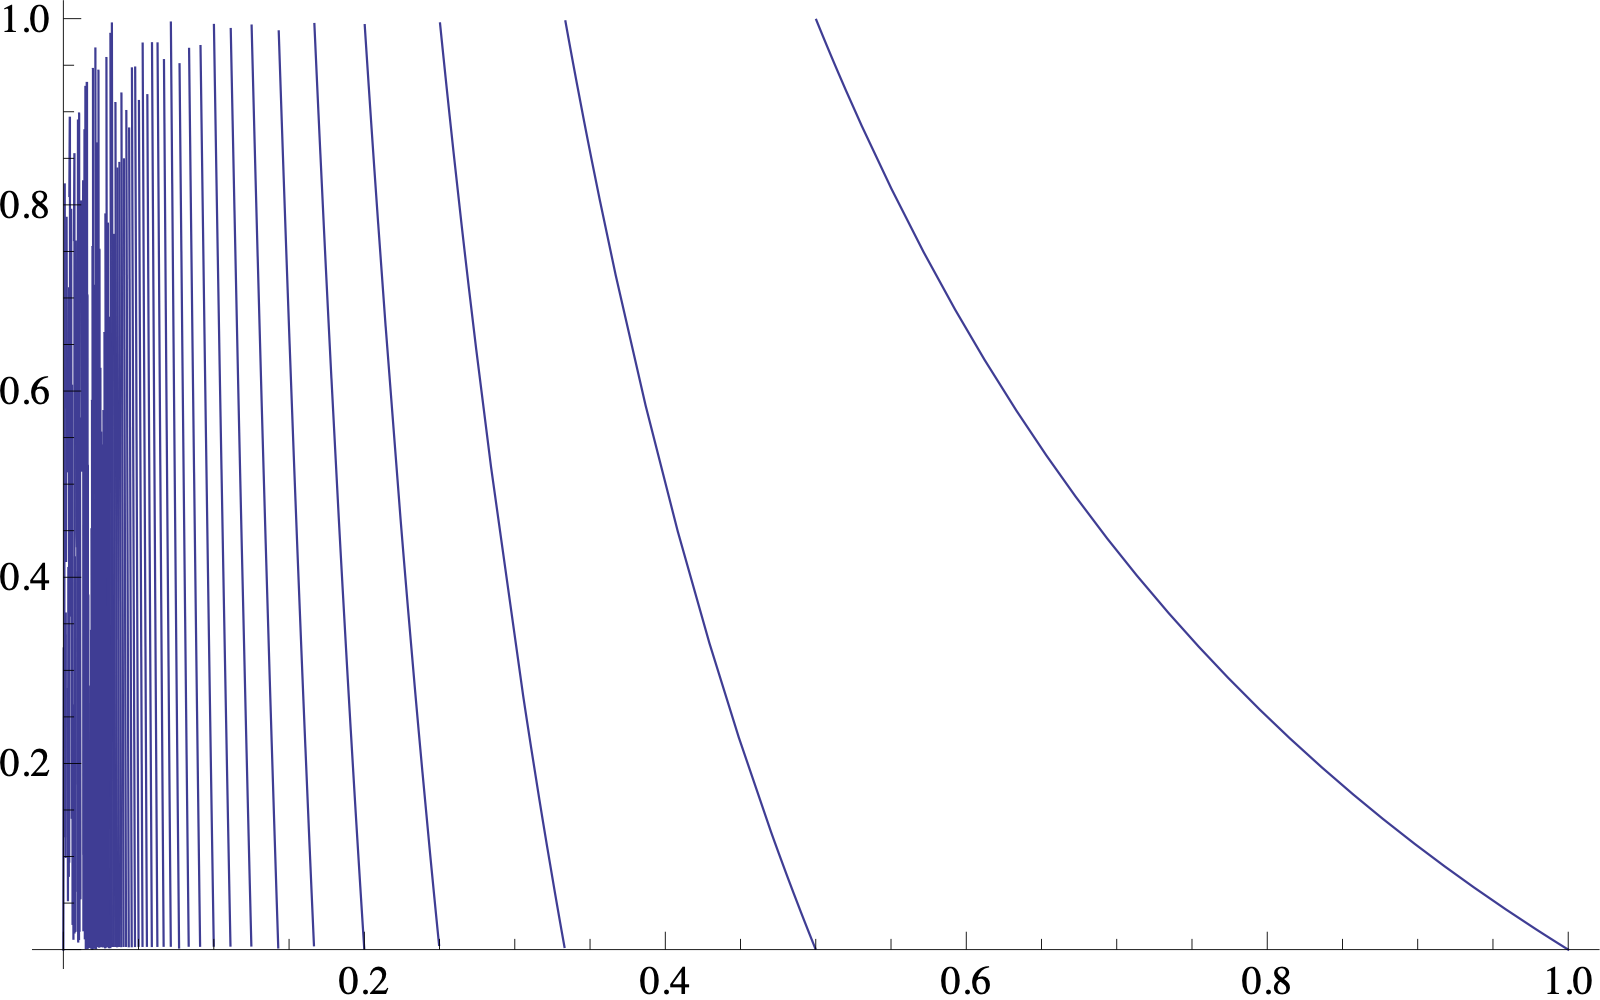
\includegraphics[width=\linewidth]{figures/gaussmap.png}\\
(d)
\end{minipage}\\[0.6em]
{\small Figure 10: (a) The doubling map; (b) The circle
rotation map $R_\alpha$ for $\alpha=0.3$; (c) the
tent map $\Lambda_2$; (d) The Gauss map.}
\end{center}

\section{Fixed points and cycles}

When we studied ODEs, we were interested in rest
points, which are static points of the phase state
which remain stationary under the ODE dynamics, and in
periodic orbits which close in on themselves and lead
to infinite repetition of a sequence of movements. In
discrete-time systems, the analogous concepts are
\emph{fixed points} and \emph{cycles}. A point $x\in I$ is a
fixed point of a map $T:I\to\mathbb{R}$ if $T(x)=x$.
We call a finite sequence $(x_j)_{j=1}^n$ a cycle (or
an $n$-cycle if we want to emphasize its length) of
$T$ if all the $x_j$'s are distinct and
$T(x_1)=x_2, T(x_2)=x_3, \ldots, T(x_{n-1})=x_n,
T(x_n)=x_1$.

The fixed points can be found graphically by drawing
the graph of $T$ and the graph of the curve $y=x$,
and finding their intersections. Note that if
$(x_j)_{j=1}^n$ is an $n$-cycle of $T$ then
$x_1 = T(T(T(\ldots(T(x_1)))\ldots)$ (that is,
iterating $T$$n$-times starting from $x_1$ leads
back to $x_1$). The map $T$ iterated $n$ times is
denoted $T^n$ (usually it is understood from the
context that this represents an iteration rather than
raising to a power; when there is risk of confusion
one needs to be careful and say explicitly what is
meant). So, the $n$-cycles can be found by first
computing the iterated map $T^n$ and then finding the
fixed points of $T^n$. Note that such a fixed point
could turn out to be the first point of an $n$-cycle,
or it could be a fixed point of $T$, or a fixed point
of $T^k$ for some $k<n$ that is a divisor of $n$ (in
this case we can use it to generate a $k$-cycle
$x_1,T(x_1,\ldots,T^{k-1}(x_1)$). In practice,
finding the $n$-cycles often becomes very hard to do
when $n$ is larger than some very small number.

\begin{example}
Consider the map $T(x)=x^2$ on $[0,1]$. The fixed
points are solutions of $x^2=x$, i.e., $x=0$ and
$x=1$. Computing the iterated maps gives
$T^2(x)=T(T(x))=x^4, T^3(x)=x^8, \ldots,
T^n(x)=x^{2^n}, \ldots$.
The fixed points of $T^n$ are still $x=0$ and $x=1$,
which means there are no $n$-cycles for $n>1$.
\end{example}

\begin{example}
The doubling map $D(x)=2x\textrm{ mod }1$ has no
fixed points. What about $2$-cycles? We have
$D^2(x)=D(D(x))=4x\textrm{ mod }1$. The equation
$x=D(D(x))$ has two solutions: $x_1=4x_1-1$ gives
$x_1=1/3$; $x_2=4x_2-2=2/3 = D(x_1)$. So we have
found a $2$-cycle $(1/3,2/3)$. In general, it is
possible to identify all $k$-cycles, by noting an
important connection between the doubling map and the
binary expansion of a real number.
\end{example}

\begin{xexercise}[$k$-cycles of the doubling map]
Identify all the $k$-cycles of the doubling map, by
using the connection with binary expansions (see the
discussion in Section \ref{sec:normalnumbers}).
Alternatively, plot $D^k(x)=2^k x \textrm{ mod }1$
and use a graphical approach to identify all the
$k$-cycles.
\end{xexercise}

\section{Stability of fixed points}

What happens to the system $x_{n+1}=T(x_n)$ if we
move slightly away from a fixed point $x_*$? We will
call the fixed point $x_*$\emph{asymptotically stable},
or \emph{attracting}, if it has the property that for
initial points $x_0$ in some small neighborhood
$(x_*-\delta, x_*+\delta)$ of $x_*$, the sequence of
iterates $x_n = T^n(x_0)$ converges to $x_*$. We will
say that $x_*$ is \emph{asymptotically unstable}, or
\emph{repelling}, if there is some $\delta>0$ such that
for any initial point $x_0\neq x_*$, the sequence of
iterates $x_n=T^n(x_0)$ will eventually leave the
interval $[x_*-\delta,x_*+\delta]$. It is also
possible for a fixed point to exhibit a mixture of the
two types of behavior; for example, it may be
attracting for initial points $x_0>x_*$ and repelling
for $x_0<x_*$.

To understand the stability properties near a fixed
point, consider the linear approximation to $T$
around $x_*$ (assuming it is continuously
differentiable in a neighborhood of the fixed point):

\begin{align*}
T(x) &= T(x_*) + T'(x_*) (x-x_*) + o(x-x_*) \\ &= x_* + T'(x_*) (x-x_*) + o(x-x_*),
\end{align*}

\noindent i.e., if the initial point $x_0$ is near $x_*$ then
by the neglecting the little-o $o(x-x_*)$ term, we
see that for the first few values we have
approximately

\begin{align*}
x_{n+1} - x_* \approx T'(x_*) (x_n-x_*),
\end{align*}

\noindent or, denoting $y_n = x_n-x_*$ and $\lambda=T'(x_*)$,

\begin{align*}
y_{n+1} \approx \lambda y_n,
\end{align*}

\noindent which is the recurrence for geometric growth.
Ignoring the small inaccuracy that comes from the
linearization, clearly $y_n\to 0$ if $|\lambda|<1$,
and $|y_n|$ becomes larger than some fixed small
number $\delta>0$ if $|\lambda|>1$. Thus, we have
essentially proved the following fact.

\begin{lem}
\label{lem-fixedpoint-stability}
For a fixed point $x_*$, if $|T'(x_*)|<1$ then the
fixed point is asymptotically stable, and if
$|T'(x_*)|>1$ then the fixed point is asymptotically
unstable.
\end{lem}

\begin{xexercise}
Complete the argument sketched above to get a
rigorous proof of \hyperref[lem-fixedpoint-stability]{Lemma~\ref*{lem-fixedpoint-stability}}.
\end{xexercise}

\begin{example}
In the example above involving $T(x)=x^2$, we have
$T'(0)=0$ and $T'(1)=2$, so $0$ is an asymptotically
stable fixed point, and $1$ is an asymptotically
unstable fixed point.
\end{example}

\begin{example}
Pull out a pocket calculator and repeatedly press the
``$\cos$'' button. The value on the display will
converge to the number $x_*\approx0.739085$, which is
the unique fixed point of $T(x)=\cos x$. Note that
$T'(x_*)=-\sin(x_*)\approx -0.673$, which shows that
the fixed point is asymptotically stable. Note that
the fact that $T'(x)<0$ means that the values of
$x_n=\cos^n(0)$ will oscillate around $x_*$,
producing values that are alternately bigger and
smaller than $x_*$.
\end{example}

\begin{xexercise}
In the case in which $|T'(x_*)|=1$ but
$T''(x_*)\neq 0$, characterize the asymptotic
stability of the fixed point as a function of
$T'(x_*)$ and $T''(x_*)$.
\end{xexercise}

\section{A detailed study of the logistic map}

This section is based on sections 10.2--10.5 in
Strogatz's book \emph{Nonlinear Dynamics and Chaos}.

\section{Measures and measure preserving maps}

Our study of maps so far has shown that even very
simple maps such as the logistic map or the $3x+1$
map can lead to extremely complicated behavior of the
associated dynamical system. Is there any hope of
understanding such complicated systems in some
meaningful sense? Yes, there is. A key insight is that
one should focus on questions of a statistical nature:
instead of trying to predict in detail where the orbit
of a particular initial point $x_0$ will go (which is
hopeless for a chaotic system), instead we will try to
make predictions about statistical behavior of orbits,
i.e., how often they visit each part of the state
space. The mathematical object that encodes such a set
of statistics is called a \emph{probability measure}, and
as we will see, a natural condition for a measure to
encode the correct information about a map is that the
map is \emph{measure preserving}.

Let $\Omega$ be a set. The theory of probability
measures can be developed in much greater generality,
but for our purposes we will assume that $\Omega$ is
a connected open (or closed) subset of $\mathbb{R}$
or of $\mathbb{R}^d$. Thus, on $\Omega$ there is a
natural ``measure'' $d\mathbf{x}$ of $d$-dimensional
volume familiar from multivariate calculus. The
probability measures that we will consider take the
form

\[
P(d\mathbf{x})=f(\mathbf{x})\,d\mathbf{x}
\]

\noindent where $f$ is a nonnegative function such that
$\int_{\Omega} f(\mathbf{x})\,d\mathbf{x} = 1$.
Formally, the measure $P$ is considered to be a
function $A\mapsto P(A)$ that takes a subset
$A\subset \Omega$ and returns a number

\[
P(A) = \int_A f(\mathbf{x})d\mathbf{x}.
\]

\noindent Both the function $f$, called the \emph{probability
density function} associated with $P$, and the set $A$
are assumed to be sufficiently well-behaved that
$P(A)$ is defined. (You can learn about the precise
technical definitions, which we will not discuss here,
in an advanced class on real analysis, measure theory
or probability theory). A set $A$ for which $P(A)$ is
defined is called a \emph{measurable set}. It is an
annoying fact of life that not all sets are
measurable, but in practice all sets that you are ever
likely to encounter will be measurable, so we will not
worry about that.

Now, if $T:\Omega\to \Omega$ is a map and $P$ is a
probability measure on $\Omega$, we say that $T$\emph{preserves the measure $P$} (or \emph{is measure
preserving for $P$}) if for any measurable set $A$
the following identity holds:

\[
P(A) = P(T^{-1}(A)),
\]

\noindent that is,

\[
\int_A f(\mathbf{x})d\mathbf{x} = \int_{T^{-1}(A)} f(\mathbf{x})d\mathbf{x}.
\]

\noindent For interval maps, it is sufficient to prove this
when $A$ is an interval. The intuitive meaning of the
definition is that if the measure $P$ represents the
statistical distribution of a random element $x$ in
$\Omega$ (corresponding to the state of the dynamical
system at some time $n$), then $T(x)$, which
corresponds to the state at time $n+1$, will have the
same statistical distribution. In other words, the
probabilistic behavior is stationary with respect to
the time dynamics. A dynamical system $(\Omega, T)$
together with a probability measure $P$ that is
preserved by $T$ is called a \emph{measure preserving
system}. If $T$ preserves the measure $P$, we say
that $P$ is an \emph{invariant measure} for $T$.

\begin{example}[Circle rotation map]
The circle rotation map $R_\alpha$ preserves the
standard length measure on $[0,1)$ (which in analysis
is called \emph{Lebesgue measure} --- pronounced like
\emph{le-baig}), i.e., the measure with density
$f(x)\equiv 1$.
\end{example}

\begin{proof}
This fact is obvious if you think of the intuitive
meaning of the circle rotation map, but for
illustration purposes here is a formal proof. If $A$
is a subset of $[\alpha,1)$ then
$R_\alpha^{-1}(A) = A-\alpha$, so clearly the length
measure is preserved. Similarly, if
$A \subset [0,\alpha)$ then
$R_\alpha^{-1}(A) = A+1-\alpha$ and again the length
measure is preserved. For a general $A\subset[0,1)$,
write $A$ as a disjoint union $A=A'\sqcup A''$ where
$A'\subset[0,\alpha)$, $A''\subset[\alpha,1)$, then
$R_\alpha^{-1}(A) = R_\alpha^{-1}(A')\sqcup
R_\alpha^{-1}(A'')$
has the same Lebesgue measure as $A$.
\end{proof}

\begin{example}[Doubling map]
The doubling map also preserves Lebesgue measure.
\end{example}

\begin{proof}

\[
P(D^{-1}(A)) =
P\left(\tfrac12 A \sqcup \left(\tfrac12 A+\tfrac12\right) \right)
= \tfrac12 P(A)
+ \tfrac12 P(\tfrac12+A) =
P(A).
\]

\end{proof}

\begin{xexercise}[Tent map $\Lambda_2$]
Show that the tent map $\Lambda_2$ (the special case
$a=2$ of the family of tent maps $\Lambda_a$)
preserves Lebesgue measure.
\end{xexercise}

\begin{example}[Logistic map $L_4$]
For $r=4$, the logistic map $L_r=L_4$ preserves the
measure

\[
P(dx) = \frac{1}{\pi \sqrt{x(1-x)}}\,dx.
\]

\end{example}

\begin{proof}
Denote $f(x)=\frac{1}{\pi \sqrt{x(1-x)}}$. If
$A \subset [0,1]$ is an interval, then

\begin{align*}
P(L_4^{-1}(A)) &= \int_{L_4^{-1}(A)} f(x)\,dx \\ &=
\int_{L_4^{-1}(A)\cap\left[0,1/2\right]} f(x)\,dx +
\int_{L_4^{-1}(A)\cap\left[1/2,1\right]} f(x)\,dx \\
&= \int_A f(\lambda_1(y))\frac{dy}{L_4'(\lambda_1(y))} + \int_A f(\lambda_2(z)) \frac{dz}{-L_4'(\lambda_2(z))},
\end{align*}

\noindent where we define
$\lambda_1(y)=\tfrac12(1-\sqrt{1-y}),
\lambda_2(z)=\tfrac12(1+\sqrt{1-z})$
(the functions $x=\lambda_{1,2}(w)$ are the two
solutions of the equation $L_4(w)=x$), and we make
the substitutions

\begin{align*}
y&=L_4(x) \leftrightarrow x=\lambda_1(y) \textrm{ in the first integral,} \\ z&=L_4(x) \leftrightarrow x=\lambda_2(z) \textrm{ in the second integral}.
\end{align*}

\noindent Note that $L_4$ is decreasing on $[1/2,1]$, which
explains why we needed to insert a minus sign in front
of the $L_4'(\lambda_2(z))$ term in the second
integral.

Now, since we are trying to prove that the expression
above is equal to $P(A)=\int_A f(x)\,dx$, it will be
enough to show that the following identity holds:

\begin{align*}
f(x) = f(\lambda_1(x))\frac{1}{|L_4'(\lambda_1(x))|} + f(\lambda_2(x))\frac{1}{|L_4'(\lambda_2(x))|}
\end{align*}

\noindent (the absolute value signs make the sum on the right
more symmetric, though of course the first one is
unnecessary). This identity is strange but easy to
verify: noting the simple relations

\begin{align*}
L_4'(w) &=4(1-2w), \\ f(w)&=\frac{2}{\pi\sqrt{L_4(w)}}, \\ L_4(\lambda_1(x)) &= L_4(\lambda_2(x)) =x,
\end{align*}

\noindent the right-hand side of the identity becomes

\begin{align*}
\frac{2}{\pi \sqrt{x}} &\cdot \frac{1}{4(1-(1-\sqrt{1-x}))}
-
\frac{2}{\pi \sqrt{x}}\cdot \frac{1}{4(1-(1+\sqrt{1-x}))} \\
& =
\frac{1}{2\pi} \left( \frac{1}{\sqrt{x}}\cdot \frac{1}{\sqrt{1-x}} +
\frac{1}{\sqrt{x}}\cdot \frac{1}{\sqrt{1-x}} \right) = \frac{1}{\pi\sqrt{x(1-x)}} = f(x).
\end{align*}

\end{proof}

\noindent The idea used in the proof above can be generalized
to give a criterion for checking whether a map is
measure-preserving.

\begin{lem}
\label{lem:measure-pres}
Let $T:I\to I$ be an interval map that is piecewise
smooth and monotonic, i.e., the interval $I$ can be
decomposed into a union of finitely many subintervals
on each of which $T$ is smooth and monotonic (in
fact, the claim is true even if this is true for a
subdivision into countably many subintervals). Then
$T$ preserves the measure $P(dx)=f(x)dx$ if and only
if the density $f(x)$ satisfies the equation

\begin{align*}
f(x) = \sum_{y\in T^{-1}(x)} \frac{f(y)}{|T'(y)|}
\end{align*}

\noindent for all but countably many points $x\in I$, where the
sum ranges over all pre-images of $x$.
\end{lem}

\begin{xexercise}
Prove \hyperref[lem:measure-pres]{Lemma~\ref*{lem:measure-pres}}.
\end{xexercise}

\begin{example}[Gauss map]
The Gauss map $G(x)$ preserves the measure $\gamma$
on $(0,1)$ (called \emph{Gauss measure}), defined by

\[
\gamma(dx) = \frac{1}{\log 2}\cdot \frac{1}{1+x}\,dx.
\]

\end{example}

\begin{xexercise}
Use \hyperref[lem:measure-pres]{Lemma~\ref*{lem:measure-pres}} to prove this.
\end{xexercise}

\begin{xexercise}[Additive Gauss map]
The additive Gauss map $g:[0,1]\to[0,1]$ is defined
by

\begin{align*}
g(x) = \begin{cases} \frac{x}{1-x} & \textrm{if }0\le x\le \tfrac12, \\
\frac{1-x}{x}&\textrm{if }\tfrac12\le x\le 1
\end{cases}
\end{align*}

\noindent (see Figure 11(a)). Show that $g$ preserves the
measure

\[
m(dx)=\frac{1}{x}\,dx.
\]

\noindent (Note: this measure is not a probability measure,
since the integral of the density is infinite.
However, the concept of measure-preservation makes
sense for such measures, and \hyperref[lem:measure-pres]{Lemma~\ref*{lem:measure-pres}}
is still valid in this context.)
\end{xexercise}

\begin{xexercise}[Boole map]
Show that \emph{Boole's transformation}

\begin{align*}
B(x)=x-\frac{1}{x}
\end{align*}

\noindent preserves Lebesgue measure on $\mathbb{R}$.
\end{xexercise}

\begin{xexercise}[Pythagorean triples map]
The interval map $N:[0,1]\to[0,1]$

\begin{align*}
\begin{cases}
\frac{x}{1-2x} & \textrm{if }0\le x\le \tfrac13, \\
\frac{1}{x}-2 & \textrm{if }\tfrac13 \le x \le \tfrac12, \\
2-\frac{1}{x} & \textrm{if }\tfrac12 \le x \le 1,
\end{cases}
\end{align*}

\noindent arises in the study of Pythagorean triples. (Figure
11(b) explains why it is denoted by $N$.) Show that
it preserves the measure

\begin{align*}
\pi(dx) = \frac{1}{x(1-x)}\,dx.
\end{align*}

\end{xexercise}

\noindent Although much of our discussion has been focused on
interval maps, the concept of measure preserving
systems appears in many different contexts (including
some rather exotic ones), as the next few examples
illustrate.

\begin{center}
\begin{minipage}[t]{0.44\linewidth}\centering
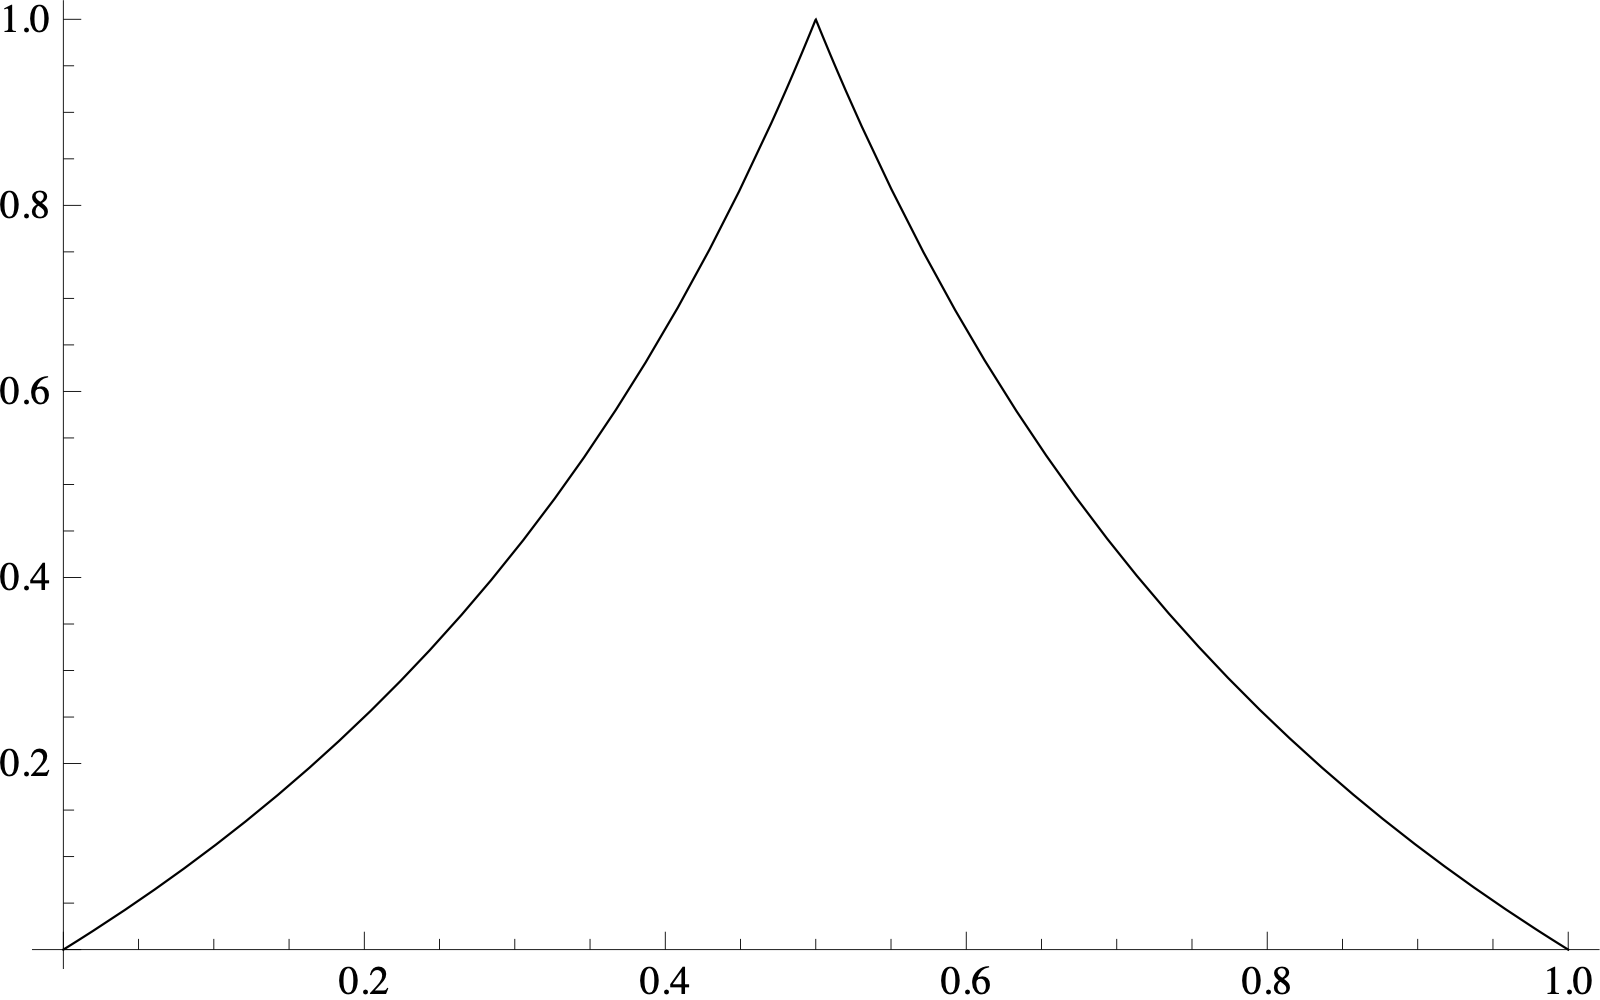
\includegraphics[width=\linewidth]{figures/slowgauss.png}\\
(a)
\end{minipage}\hspace{0.02\linewidth}%
\begin{minipage}[t]{0.44\linewidth}\centering
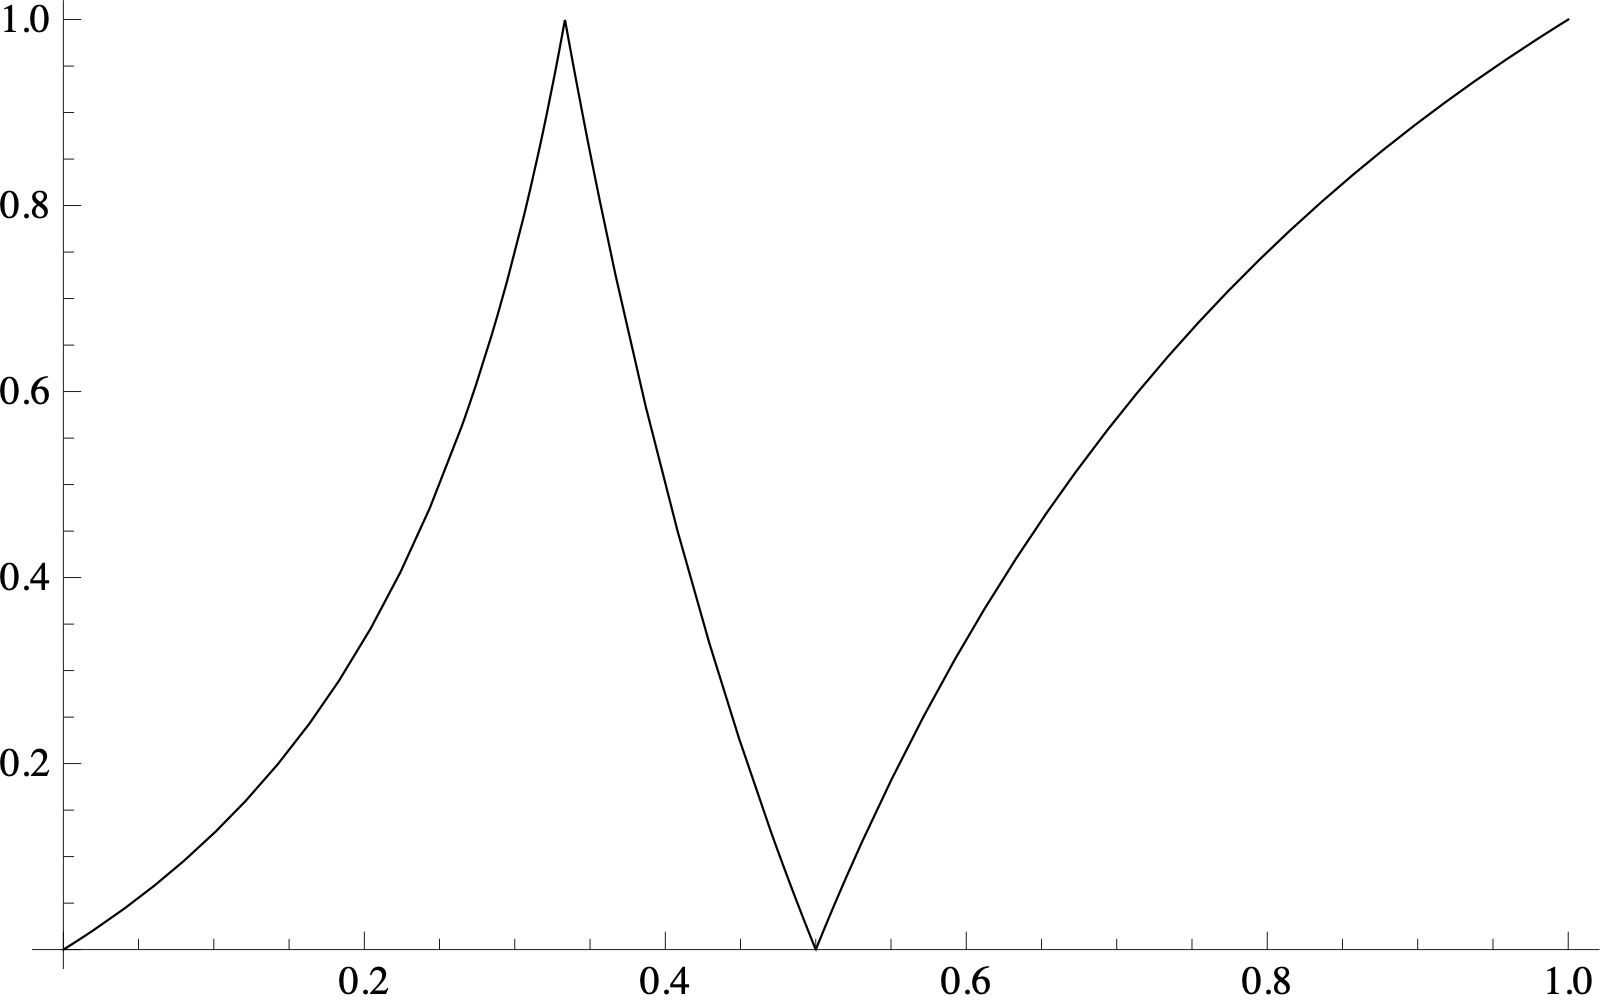
\includegraphics[width=\linewidth]{figures/pythagorean.png}\\
(b)
\end{minipage}\\[0.6em]
{\small Figure 11: (a) The additive Gauss map; (b) The
Pythagorean triples map.}
\end{center}

\begin{example}[Hamiltonian flow]
By Liouville's theorem, the phase flow of a
Hamiltonian system preserves area measure in
$\mathbb{R}^2$ (also called the two-dimensional
Lebesgue measure). This is a continuous-time dynamical
system, but the notion of measure preserving dynamics
makes sense for such systems as well. In particular,
if the system is discretized by fixing a time step
$\tau$, we get a map preserving Lebesgue measure.
\end{example}

\begin{example}[Geodesic flow]
The geodesic flow is a continuous-time dynamical
system on a curved surface. Its phase space is the set
of points $(x,v)$ where $x$ is a point on the surface
and $v$ is a tangent vector to the surface based at
$x$ (representing the direction and speed in which a
person standing at $x$ will start walking). The flow
$\varphi_t(\cdot,\cdot)$ takes such a pair $(x,v)$
and maps it to a new pair $(x',v')=\varphi(x,v)$
representing where the person will be, and which
direction they will be pointing at, $t$ time units
later. It can be shown that the geodesic flow
preserves the natural volume measure associated with
the phase space (roughly speaking, the measure is
product of the surface area measure of the surface in
the component $x$, and a standard area measure in the
$v$ component).
\end{example}

\begin{example}[Billiard map]
Billiard maps can be thought of as a limiting case of
certain Hamiltonian systems (think of a limit in which
the reflecting wall is actually a strongly repelling
potential well that becomes steeper and steeper), so
they too have an invariant measure. In certain natural
coordinates $\phi, \theta, \ell$, the formula for the
invariant measure becomes

\begin{align*}
P(A) = \int_A \frac{\sin \theta}{\sin \theta_1}\, d\theta\, d\phi\, d\ell.
\end{align*}

\noindent (For the meaning of these quantities, see the
interesting article \emph{What is the ergodic theorem?}, G.
D. Birkhoff, \emph{American Math. Monthly}, April 1942.)
\end{example}

\begin{example}[$3x+1$ map]
One of the many (ultimately unsuccessful) attempts at
solving the famous $3x+1$ problem mentioned in
Section \ref{sec:ergodic-intro} was based on the
observation that since the formula of the $3x+1$ map
$T(x)$ depends on the parity of $x$, the range of
definition of $T$ can be expanded to include numbers
of the form

\begin{align*}
a_0 + a_1 \cdot 2 + a_2 \cdot 4 + a_3\cdot 8 + \ldots + a_n \cdot 2^n + \ldots = \sum_{n=0}^\infty a_n 2^n.
\end{align*}

\noindent Such exotic numbers, which have an infinite binary
expansion to the \emph{left} of the ``binary point'', are
called \emph{$2$-adic integers} and have fascinating
properties. In particular, there is a natural measure
associated with them that is analogous to Lebesgue
measure on $\mathbb{R}$. It can be shown that the
extended $3x+1$ map preserves this measure.
\end{example}

\section{Measure $0$ sets}

A set $E\subset \mathbb{R}$ is called a \emph{measure 0}
set if its Lebesgue measure is 0. Although we have not
discussed (and do not plan to discuss) precise
definitions of Lebesgue measure or of the notion of
measurability, for the case of measure 0 sets there is
an easy explicit definition. $E$ has measure 0 if and
only if for any $\epsilon>0$, $E$ can be covered by a
countable union of open intervals whose lengths add up
to less than $\epsilon$:

\[
\forall \epsilon>0\ \ \ E\subset\bigcup_{n=1}^\infty (a_n, b_n), \ \  \sum_{n=1}^\infty (b_n-a_n) < \epsilon \ \iff \ \textrm{measure 0.}
\]

\begin{xexercise}
Prove that any countable set $E\subset \mathbb{R}$
has measure 0.
\end{xexercise}

\section{Invariant sets, ergodicity and the ergodic theorem}

We now come to a key idea that underlies the basis
for all of ergodic theory and explains the importance
of invariant measures in discrete-time dynamics. Given
a map $T:I\to I$ and the associated recurrence
$x_{n+1}=T(x_n)$, for every sub-interval $A\subset I$
we can compute the frequency of visits of the
dynamical system to $A$, namely

\begin{align*}
\mu_{x}^{(n)}(A) = \frac{1}{n} \# \left\{ 0\le k \le n-1\,:\, T^k(x) \in A \right\}.
\end{align*}

\noindent Note that this depends on the set $A$ as well as on
$n$ (the number of elements in the sequence of
iterates we are using to compute the frequency) and
$x$, the initial point. If we fix $n$ and $x$, the
function $A\mapsto \mu_x^{(n)}(A)$ is a probability
measure (but it is a discrete probability measure,
which assigns a positive measure of $1/n$ to the
specific points $x,T(x),\ldots,T^{n-1}(x)$, instead
of the measures we considered earlier which were
defined in terms of a density function $f(x)$). Now
let $n\to\infty$ (for fixed $x$). If we are lucky,
the probability measures $\mu_x^{(n)}(\cdot)$ will
converge to a limiting measure $P(dx)=f(x)dx$, in the
sense that

\begin{align*}
\mu_x^{(n)}(A) \xrightarrow[n\to\infty]{} P(A) = \int_A f(x)\,dx \ \ \textrm{ for any subinterval }A\subset I.
\end{align*}

\noindent It is not hard to see that the limiting measure needs
to be an invariant measure for $T$:

\begin{align*}
P(T^{-1}(A)) &= \lim_{n\to\infty} \mu_x^{(n)}(T^{-1}(A)) \\ &
= \lim_{n\to\infty} \frac{1}{n}\#\left\{ 0\le k\le n-1\,:\,T^k(x)\in T^{-1}(A) \right\} \\
&
= \lim_{n\to\infty} \frac{1}{n}\#\left\{ 0\le k\le n-1\,:\,T^{k+1}(x)\in A \right\} \\
&
= \lim_{n\to\infty} \frac{1}{n}\#\left\{ 1\le k\le n\,:\,T^{k}(x)\in A \right\} \\
&
= \lim_{n\to\infty} \frac{1}{n}\#\left\{ 0\le k\le n-1\,:\,T^{k}(x)\in A \right\} = P(A).
\end{align*}

\noindent It is therefore clear that an invariant measure which
arises in this way encodes useful statistical
information about the orbit of the point $x$ under
the map $T$. On the other hand, the limiting measure
may depend on $x$ (or we may have convergence to a
limiting measure for some values of $x$, and fail to
have convergence for other values). It turns out that
for a wide family of maps, called \emph{ergodic} maps, the
limit is mostly independent of the initial point $x$.
We summarize the relevant facts, whose proof is beyond
the scope of the course, in the following result,
which is a version of a famous theorem known as
Birkhoff's Pointwise Ergodic Theorem:

\begin{thm}[The ergodic theorem]
If $T:I\to I$ is an interval map which preserves a
measure $P(dx)=f(x)dx$, then:

\begin{enumerate}[label=\arabic*.]
\item There is a set $E\subset I$ such that $I\setminus E$
is a measure-$0$ set and for any $x\in E$, the
measures $\mu_x^{(n)}(\cdot)$ converge to a limiting
invariant measure $P_x$ in the sense described above.

\item If $T$ satisfies a natural condition known as
ergodicity, then $P_x$ is independent of $x$ and is
equal to the invariant measure $P$ for all $x\in E$.
\end{enumerate}

\end{thm}

\noindent Maps for which the condition of part (b) applies are
the ergodic maps. In such a case, one can say that
``the statistics of most orbits reproduce the ideal
statistics of the system'', or that ``time averages
are equal to space averages''. That is, by observing a
typical orbit for a long time we can learn about the
statistical behavior of almost all other orbits. We
will not discuss the precise definition of ergodicity,
preferring instead to explore some of the interesting
consequences of the result above. Roughly speaking
(setting aside some nuances involving measure 0 sets),
a map is ergodic if $I$ can't be divided into two
disjoint parts $A$ and $B$ such that $P(A)>0$,
$P(B)>0$ and for any points $x\in A, y\in B$,
$T^k(x)\in A$ and $T^j(y) \in B$ for all $j,k\ge 0$.
Such sets $A$ and $B$ are called \emph{invariant sets} for
$T$. The existence of a nontrivial invariant set is a
fairly obvious obstacle to the statement of part (b)
in the theorem above holding true, and the main
difficulty in proving the result is showing that when
there are no invariant sets then (in some sense) there
is nothing else that can go wrong and therefore the
result must be true.

Another thing to note is that actually checking
whether a given map is ergodic may be rather
difficult. However, we will use the theorem in a few
cases in which ergodicity is known and not very
difficult to prove.

\section{The doubling map and normal numbers}
\label{sec:normalnumbers}

Our first application of the ergodic theorem is
related to the doubling map $D(x)=2x\textrm{ mod }1$,
which as we have seen preserves Lebesgue measure on
$(0,1)$. We will use without proof the fact that this
map is ergodic. The reason this is interesting is
because the orbits $D^n(x)$ of a number $x$ encode
information about the binary expansion of $x$. More
precisely, write

\begin{align*}
x = \sum_{n=1}^\infty a_n(x) 2^{-n},
\end{align*}

\noindent where $a_n(x) \in \{0,1\}$ is the $n$th digit in the
binary expansion of $x$ (in the case of a dyadic
number $m/2^N$ for which there is a small amount of
ambiguity, choose the expansion which terminates with
an infinite succession of $0$'s). Applying the
doubling map gives

\begin{align*}
D(x) = 2x\textrm{ mod 1} = \sum_{n=1}^\infty a_n(x) 2^{-(n-1)} \textrm{ mod }1 = \sum_{n=1}^\infty a_{n+1}(x)2^{-n},
\end{align*}

\noindent from which we conclude that $a_n(D(x)) = a_{n+1}(x)$
-- in terms of the binary expansion, the doubling map
has the effect of ``chopping off'' the leading digit
in the expansion. Successive applications of $D$ will
chop off additional digits. By tracking the frequency
of visits of $D(x)$ to a specific set such as
$(0,1/2) = \{ u\in(0,1)\,:\, a_1(u)=0 \}$, we can
prove the following result:

\begin{thm}
All numbers $x\in(0,1)$ except those lying in some
measure-0 set have the property:

\begin{equation*} \tag{35}\label{eq:normal1}
\begin{split}
\frac{1}{n}\#\left\{ 1\le k\le n\,:\, a_n(x) = 0 \right\} \xrightarrow[n\to\infty]{} \tfrac12,
\end{split}
\end{equation*}

\noindent and, more generally, for any
$b_1,\ldots,b_m\in\{0,1\}$, we have

\begin{equation*} \tag{36}\label{eq:normal2}
\begin{split}
\frac{1}{n}\#\left\{ 1\le k\le n\,:\, a_k(x) = b_1,\ldots, a_{k+m-1}(x)=b_m \right\} \xrightarrow[n\to\infty]{} \frac{1}{2^m}.
\end{split}
\end{equation*}

\end{thm}

\begin{proof}
The frequency on the left-hand side of \eqref{eq:normal1}
is what we denoted earlier by $\mu_x^{(n)}((0,1/2))$
(with respect to the doubling map), so by the ergodic
theorem, it converges to $P((0,1/2))=1/2$. Similarly,
the left-hand side of \eqref{eq:normal2} converges to the
Lebesgue measure of the interval
$[\sum_{j=1}^m b_j 2^{-j},\sum_{j=1}^m b_j
2^{-j}+2^{-m})$,
which is $1/2^m$.
\end{proof}

\noindent A number $x\in (0,1)$ is called \emph{normal to base $2$}
if it satisfies the condition \eqref{eq:normal2} --- that
is, if its binary expansion contains the digits 0 in 1
in the right asymptotic frequency of $1/2$, and
similarly contains each of the types of successive
pairs ``$00$'', ``$01$'', ``$10$'' and ``$11$'' with
asymptotic frequency $1/4$, each triple of digits
with frequency $1/8$, etc. In other words, the binary
expansion of a number that is normal to base $2$ is
hard to distinguish (at least based on statistics)
from the output of an ideal random number generator.
We proved above that ``almost every'' $x\in (0,1)$
(all $x$ except for those in some measure-$0$ set) is
normal to base $2$. This can be generalized to
arbitrary bases.

\begin{xexercise}[Normal numbers to base $10$]
Define the notion of a number $x\in(0,1)$ that is
normal to base $10$. Define an interval map
$E:(0,1)\to(0,1)$ that is related to the decimal
expansion of a number in the same way that $D$ is
related to the binary expansion, and use it to prove
that almost every number $x\in(0,1)$ is normal to
base $10$.
\end{xexercise}

\section{Circle rotations and equidistribution on $(0,1)$}

Our next application of the ergodic theorem will be
to the circle rotation map
$R_\alpha(x)=x+\alpha\textrm{ mod }1$. Note that
$R_\alpha^n(x)=x+n\alpha\textrm{ mod }1 = \left\{
x+n\alpha \right\}$
(where $\left\{u\right\}=u-\lfloor u \rfloor$ denotes
the fractional part of a real number $u$).

\begin{thm}
The map $R_\alpha$ is ergodic if and only if $\alpha$
is irrational.
\end{thm}

\begin{proof}
If $\alpha=p/q$ is rational, the set

\[
E = \left[0, \tfrac{1}{2q}\right]
\cup \left[\tfrac{1}{q}, \tfrac{3}{2q}\right]
\cup \left[\tfrac{2}{q}, \tfrac{5}{2q}\right]
\cup \left[\tfrac{3}{q}, \tfrac{7}{2q}\right]
\cup \ldots
\cup \left[\tfrac{q-1}{q}, \tfrac{2q-1}{2q}\right]
\]

\noindent is an example of a nontrivial invariant set. The
other direction (that if $\alpha$ is irrational then
the map is ergodic) can be proved using Fourier
series. Here is a sketch of the proof. The idea is to
check the ergodic theorem by taking some well-behaved
function $g:[0,1)\to\mathbb{R}$ and looking at sums
of the form

\begin{align*}
\mu_x^{(n)}(g) = \frac{1}{n} \sum_{k=0}^{n-1} g(R_\alpha^k(x))
\end{align*}

\noindent (such sums are called \emph{ergodic averages}, since they
represent an averaging of the values of $g$ over
orbits of $x$). It can be shown that if the averages
converge to the ``ideal average'' $\int_0^1 g(x)\,dx$
(the average of $g$ with respect to the invariant
measure, which in this case is simply Lebesgue
measure) for a sufficiently large family of functions
$g$, then the map is ergodic. It turns out that for
the circle rotation map, this is particularly simple
to check when $g_m(x)=e^{2\pi i m x}$ is a complex
exponential, $m\in\mathbb{Z}$. For $m=0$ the claim is
trivial, and for $m\neq 0$ we have

\begin{align*}
\mu_x^{(n)}(g_m) &=
\frac{1}{n} \sum_{k=0}^{n-1} g_m(R_\alpha^k(x)) =
\frac{1}{n} \sum_{k=0}^{n-1} \exp(2\pi i m R_\alpha^k(x)) \\ &=
\frac{1}{n} \sum_{k=0}^{n-1} \exp(2\pi i m (x+k\alpha \textrm{ mod }1)) \\
&=
\frac{1}{n} \sum_{k=0}^{n-1} \exp(2\pi i m (x+k\alpha))
=
\frac{1}{n} e^{2\pi i m x} \sum_{k=0}^{n-1} e^{2\pi i m k \alpha} \\
&=
\frac{1}{n} e^{2\pi i m x} \frac{1-e^{2\pi i n m \alpha}}{1-e^{2\pi i m \alpha}} \xrightarrow[n\to\infty]{}0=\int_0^1 e^{2\pi i m x}\,dx = \int_0^1 g_m(x)\,dx.
\end{align*}

\end{proof}

\noindent Applying the ergodic theorem, we get (see the
exercise below the proof) the following famous result
in number theory, proved in 1909 and 1910
independently by Weyl, Sierpinski and Bohl.

\begin{thm}[Equidistribution theorem]
If $\alpha\in(0,1)$ is irrational then for any
$0\le a<b\le 1$

\begin{equation*} \tag{37}\label{eq:equidistribution1}
\begin{split}
\frac{1}{n} \#\Big\{ 1\le k \le n \,:\, \left\{n\alpha\right\} \in (a,b) \Big\} \xrightarrow[n\to\infty]{} b-a.
\end{split}
\end{equation*}

\end{thm}

\begin{xexercise}
The ergodic theorem only guarantees the result that

\begin{equation*} \tag{38}\label{eq:equidistribution2}
\begin{split}
\frac{1}{n} \#\Big\{ 1\le k \le n \,:\, \left\{x+n\alpha\right\} \in (a,b) \Big\} \xrightarrow[n\to\infty]{} b-a
\end{split}
\end{equation*}

\noindent holds for all $x\in [0,1)$ except on a measure-0 set.
Explain why in the case of the rotation map
$R_\alpha$, the truth of this claim is independent of
the initial point $x$, and therefore
\eqref{eq:equidistribution1} follows from
\eqref{eq:equidistribution2}.
\end{xexercise}

\section{Statistics of the logistic map $L_4$}

As a final example of the application of the ergodic
theorem, we justify our earlier claim that the
logistic map $L_4$ can be understood statistically
even though its orbits are chaotic. We rely on another
unproved fact from ergodic theory, which is that $L_4$
is ergodic.

\begin{thm}
For all $0\le a<b\le 1$ and for all $x\in[0,1]$
except on a set of measure $0$, we have

\begin{align*}
\frac{1}{n}\# &\left\{ 0\le k\le n-1\,:\, L_4^k(x) \in (a,b) \right\} \\
& \xrightarrow[n\to\infty]{} \frac{1}{\pi} \int_a^b \frac{du}{\sqrt{u(1-u)}}
= \frac{2}{\pi}\arcsin(\sqrt{b})-\arcsin(\sqrt{a}).
\end{align*}

\end{thm}

\begin{xexercise}

\begin{enumerate}[label=\arabic*.]
\item Prove that the logistic map $L_4$ is related to the
tent map $\Lambda_2$ by

\[
\Lambda_2(x) = (h\circ L_4 \circ h^{-1})(x),
\]

\noindent where $h(x) = \frac{2}{\pi}\arcsin(\sqrt{x})$. (Two
interval maps that are related to each other via a
relation of the type $T_1=h\circ T_2 h^{-1}$, where
$h:I\to I$ is invertible, are called \emph{conjugate
maps}, and share many similar properties.)

\item Use this to prove that the tent map satisfies a
similar statistical distribution result, namely that
for all $x\in[0,1]$ except on a set of measure 0, we
have

\begin{align*}
\frac{1}{n}\#\left\{ 0\le k\le n-1\,:\, \Lambda_2^k(x) \in (a,b) \right\} \xrightarrow[n\to\infty]{} b-a.
\end{align*}
\end{enumerate}

\end{xexercise}

\chapter{Part 3 — Control theory}

\section{Introduction: the problem of control}

The dynamical systems we find in nature are plagued
by a host of undesirable effects such as
instabilities, unpredictable and chaotic behavior, and
unwanted oscillations. Left to their own devices,
ecosystems can suffer cycles of uninhibited growth
followed by mass starvation; economies undergo
cyclical downturns; human hearts go into fibrillation;
aircraft would plunge down to earth; etc. The goal of
control theory is to devise methods to steer dynamical
systems away from unfavorable modes of behavior and
towards desired ones, by manipulating the differential
equation itself --- usually through manipulation of a
specific term (or set of terms) present in the
equation, known as the \emph{control function}. Control
theory is a large field, and its proper study requires
a separate concentrated effort. In these notes we will
merely give a short introduction to the subject,
focusing on a few simple examples which illustrate
some of the main ideas of this fascinating (and
extremely useful) subject and how it relates to the
theory of ODEs.

In mathematical terms, the problem of control can be
formulated as follows. We are given a vector equation
of the form

\begin{align*}
\dot{\mathbf{x}} = G(\mathbf{x},\mathbf{u},t)
\end{align*}

\noindent where $\mathbf{x}$ is a $d$-dimensional vector
dynamic variable and $G:\mathbb{R}^{d+k+1}\to\R^d$ is
a smooth function. We think of $\mathbf{u}$ as a
$k$-dimensional input that is a parameter to the
equation. That is, given a curve $\mathbf{u}(t)$ in
$\mathbf{R}^k$, we can plug it into the equation to
get an ODE
$\dot{\mathbf{x}}(t) =
G(\mathbf{x}(t),\mathbf{u}(t),t)$
for the vector variable $\mathbf{x}$. The assumption
is that we can pick $\mathbf{u}$, with the goal being
of steering the solution $x(t)$ towards a specified
desired behavior. For example, $\mathbf{u}$ could
represent a driving force in a mechanical system; an
electric voltage applied by a digital controller in an
electronic circuit; an interest rate on
government-issued bonds set by a central bank, etc. A
common goal is to make $\mathbf{x}$ go to a specific
point in $\mathbb{R}^d$ and stay there, i.e., to
stabilize the system at a state that it would not
normally (in the absence of deliberate control) remain
stable at. We refer to $\mathbf{u}$ as the \emph{control
variable} (or variables), or \emph{control function}.

\section{Feedback}

If the control variable $\mathbf{u}$ at a given time
$t$ needs to be specified simply as a function
$\mathbf{u}(t)$ of time, without reference to the
current state $\mathbf{x}(t)$ of the dynamical
system, we are talking about control without feedback
(technically, this is known as \emph{open-loop control}).
Alternatively, if we allow $\mathbf{u}$ to be
specified as a function $\mathbf{u}(\mathbf{x},t)$
(that is, if the controller is allowed to ``look at
what she is doing''), this means that the control
system incorporates feedback. A control system of this
type is known as \emph{closed-loop control}. Feedback is an
extremely powerful idea --- as anyone who has tried to
drive a car blindfolded knows! Indeed, almost all of
control theory focuses on control with feedback.
However, as we shall see below, open-loop control also
has some surprising uses.

\section{An inverted pendulum with a vertically oscillating base}

The simple pendulum has two rest points: it can be
``hanging down'' or ``standing up''. A pendulum in the
``standing up'' position is called an \emph{inverted
pendulum}. Since this rest point is asymptotically
unstable, one rarely observes pendulums in this
position! However, from the point of view of control
theory, the inverted pendulum is much more interesting
than the pendulum in its stable state. It turns out
that the pendulum can be stabilized around the
inverted rest point, using both open-loop and
closed-loop control schemes. The Segway personal
transportation device is a practical invention built
precisely around this idea.

As our first example in control theory, we will show
how the inverted pendulum can be stabilized in an
open-loop control scheme whereby the base of the
pendulum is made to oscillate along the vertical
direction. This dynamical system is known as
\emph{Kapitza's pendulum} (see Figure 12). The amplitude
and frequency of the oscillation need to be adjusted
to suitable values to achieve stability, but in
practice the effect is quite easy to achieve, and
entertaining video demonstrations of this surprising
and unintuitive result can be found online.

\begin{center}
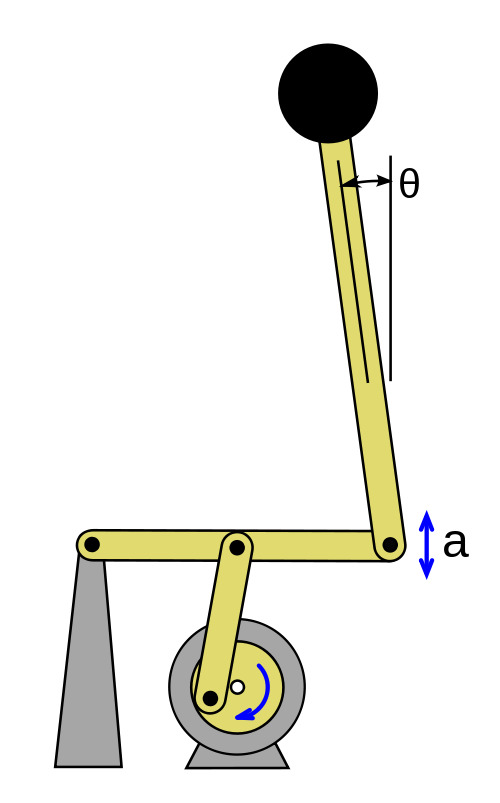
\includegraphics[width=0.32\linewidth]{figures/kapitza.png}\\[0.6em]
{\small Figure 12: Kapitza's pendulum (source: Wikipedia).}
\end{center}

\noindent Let $\ell$ denote the length of the rod of the
pendulum. We assume the base is moving along the
vertical axis as a function $u(t)$ of time (which
plays the role of the ``control function'' in this
problem), and denote by $x$ the angle the pendulum
forms with the \emph{upward-pointing vertical}, so that
$x=0$ (rather than $x=\pi$ with the more commonly
used angular coordinate) represents the unstable
equilibrium point of the inverted pendulum. The
position of the swinging mass is
$\mathbf{r}=(\ell\sin x, \ell \cos x + u(t))$. We can
now write the kinetic energy, potential energy and the
Lagrangian, as follows:

\begin{align*}
K &= \tfrac12 |\dot{\mathbf{r}}|^2 = \tfrac12\left( \ell^2 \dot{x}^2\cos^2 x + \ell^2 \dot{x}^2 \sin^2 x - 2 \ell \dot{u} \dot{x} \sin x + \dot{u}^2\right) \\
&= \tfrac12 \ell^2 \dot{x}^2 + \tfrac12 \dot{u}^2 - \ell \dot{u} \dot{x} \sin x, \\
U &= g\ell \cos x + g u, \\
L &= \tfrac12 \ell^2 \dot{x}^2 + \tfrac12 \dot{u}^2 - \ell \dot{u} \dot{x} \sin x
-g\ell \cos x - g u.
\end{align*}

\noindent Therefore we have

\begin{align*}
\frac{\partial L}{\partial x} &= -\ell \dot{u}\dot{x}\cos x + gl\sin x,
\\
\frac{\partial L}{\partial \dot{x}} &= \ell^2 \dot{x} - \ell \dot{u}\sin x,
\\
\frac{d}{dt}\left(\frac{\partial L}{\partial \dot{x}}\right) &= \ell^2 \ddot{x} - \ell \ddot{u}\sin x - \ell \dot{u}\dot{x} \cos x,
\end{align*}

\noindent and the Euler-Lagrange equation for this Lagrangian
is

\begin{align*}
\ddot{x} =\frac{g+\ddot{u}}{\ell} \sin x.
\end{align*}

\noindent That is, the effect of the vertical driving
acceleration $\ddot{u}(t)$ applied to the base point
is to make the effective gravity felt by the pendulum
change as a function of time. We shall now make some
assumptions to simplify the analysis. First, we shall
study the behavior in the vicinity of the rest point,
so we can replace the equation with its linearized
version

\begin{align*}
\ddot{x} = \frac{g+\ddot{u}}{\ell} x.
\end{align*}

\noindent Next, we assume that $u(t)$ is a periodic function
with period $2T$ and frequency $f = 1/2T$, and
furthermore, we assume that its second derivative
$\ddot{u}(t)$ takes only two values $\pm a$, changing
its sign exactly every half-period $T$, so that the
graph of $u$ over each half-period is a parabolic arc
rather than the sinusoidal arc typically used for
periodic motions (this can even be a realistic
assumption depending on the way the driving mechanism
operates in practice, but the main reason for assuming
it is that it results in a simpler mathematical
analysis); see Figure 13. With this assumption, the
equation becomes

\begin{align*}
\ddot{x} = (\omega^2 \pm A^2) x,
\end{align*}

\noindent with the notation $\omega=\sqrt{g/\ell}$,
$A=\sqrt{a/\ell}$, and where ``$\pm$'' denotes the
square wave function

\begin{align*}
\pm = \begin{cases} +1 & \textrm{if }\sin(2\pi f t)>0, \\ -1 &
\textrm{if }\sin(2\pi f t)<0.
\end{cases}
\end{align*}

\noindent We assume that $A>\omega$, i.e., the ``artificial
gravity'' induced by the vibrations dominates the
gravity of the more usual type. It can be easily
checked that the amplitude $d$ of the oscillation is
given by

\begin{align*}
d = \frac{T^2 a}{8}.
\end{align*}

\begin{center}
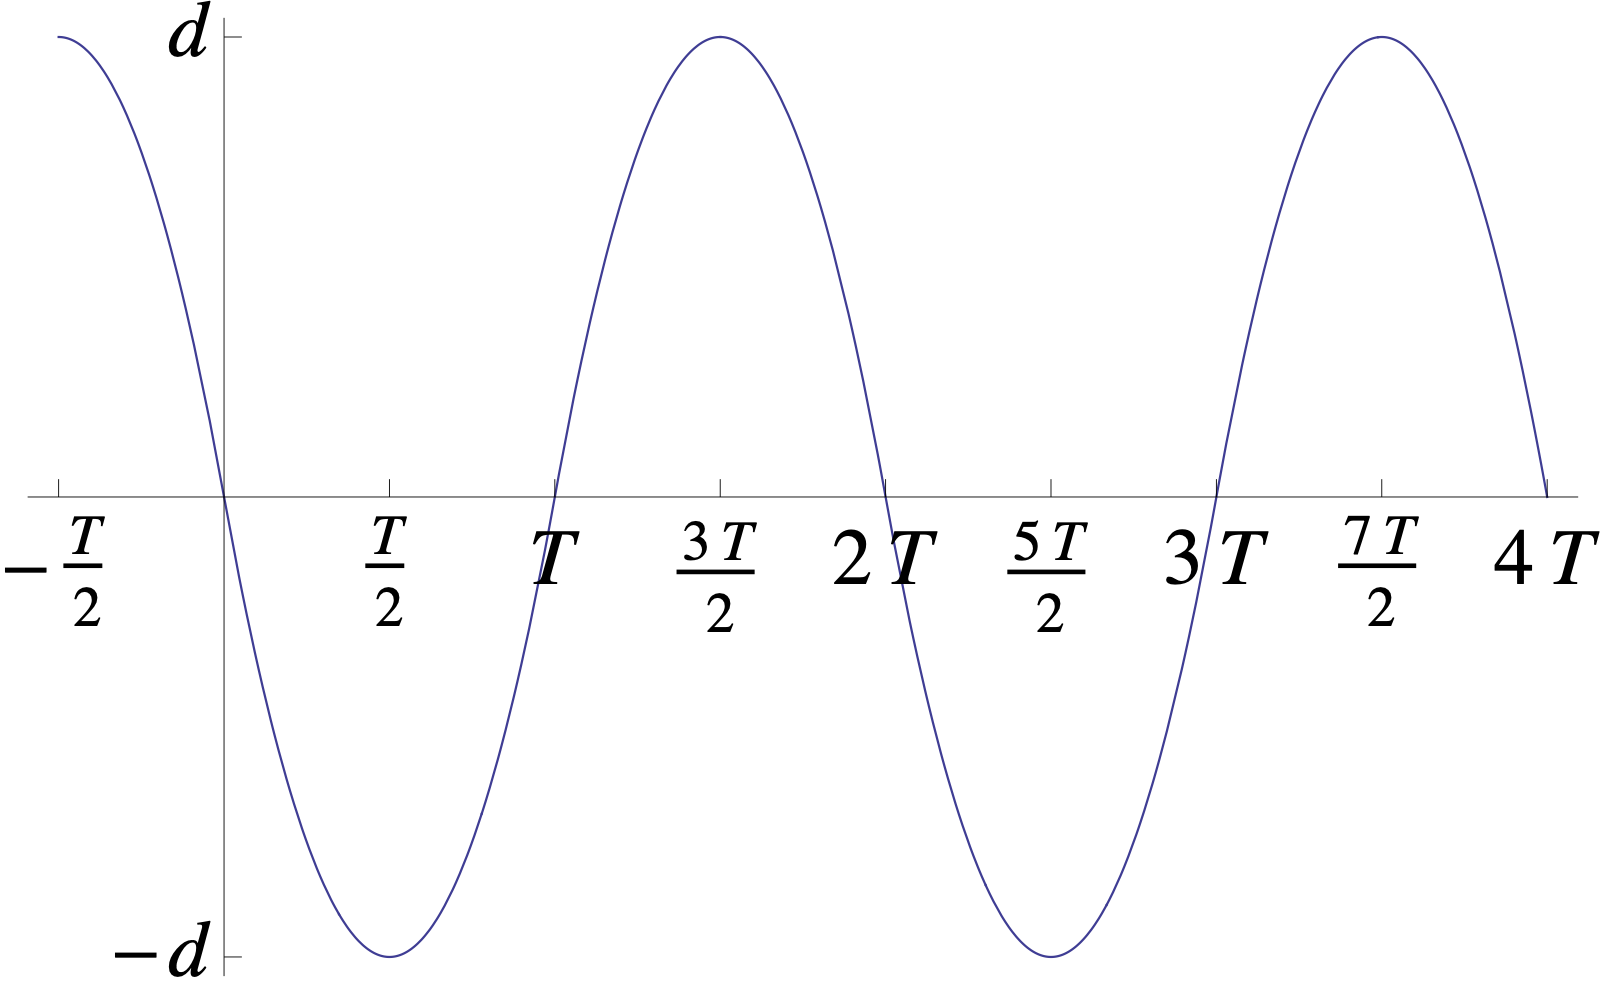
\includegraphics[width=0.70\linewidth]{figures/drivingforce.png}\\[0.6em]
{\small Figure 13: In our analysis, the driving function
$u(t)$ for the height of the oscillating base is
assumed to be periodic with period $2T$, and each
half-period is a parabolic arc with second derivative
$\pm a$ and amplitude $d$.}
\end{center}

\noindent As a final notational step before we start the
analysis, we do the usual trick of representing a
second-order system as a planar first-order system:

\begin{align*}
\dot{x} &= y, \\
\dot{y} &= (\omega^2 \pm A^2) x.
\end{align*}

\noindent Note that this is a linear, but time-dependent,
system, so we can represent it in vector notation as

\begin{equation*} \tag{39}\label{eq:kapitza-matrix}
\begin{split}
\dot{\mathbf{x}} &= B_t \mathbf{x},
\end{split}
\end{equation*}

\noindent where $\mathbf{x}=(x,y)^\top$ and
$B_t = \left( \begin{array}{cc} 0&1 \\ \omega^2\pm
A^2 & 0 \end{array}\right)$.

We are now in a position to study when (as a function
of the parameters $a, T, \ell, g$) we can expect the
system to be stable at $x=0$. The idea is to reduce
the problem to understanding the stability of an
autonomous discrete-time dynamical system which we can
explicitly compute. For real numbers $t_0<t_1$,
define a map $\psi_{t_0,t_1}:\R^2\to\R^2$, analogous
to the phase flow map $\varphi_t$ we studied for
autonomous systems, as follows:

\begin{align*}
\psi_{t_0,t_1}(\mathbf{x}_0) = &\ \mathbf{x}(t_1)\textrm{ where $\mathbf{x}(t)_{t\ge t_1}$ is the solution of the system (\ref{eq:kapitza-matrix})}\\ & \textrm{with initial condition $\mathbf{x}(t_0)=\mathbf{x}_0$}.
\end{align*}

\noindent That is, $\psi_{t_0,t_1}$ evolves a point forward in
time from time $t_0$ to time $t_1$. (In the case of
an autonomous system, we could write this as
$\varphi_{t_1-t_0}(\mathbf{x}_0)$ since it would
depend only on the duration of the evolution rather
than the specific starting and ending times.) The
evolution maps $\psi_{t_0,t_1}$ have several
important properties. First, they are linear, since
the system \eqref{eq:kapitza-matrix} is linear. Second,
they satisfy the composition property

\begin{align*}
\psi_{t_0,t_2}(\mathbf{x}_0) = \psi_{t_1,t_2}( \psi_{t_0,t_1}(\mathbf{x}_0)) \ \ (t_0<t_1<t_2),
\end{align*}

\noindent or equivalently

\begin{equation*} \tag{40}\label{eq:composition-prop}
\begin{split}
\psi_{t_0,t_2}(\mathbf{x}_0) = \psi_{t_1,t_2}\circ \psi_{t_0,t_1}\ \ (t_0<t_1<t_2),
\end{split}
\end{equation*}

\noindent since evolving a solution from time $t_0$ to $t_2$
can be done by evolving it up to time $t_1$ and then
evolving the resulting point from $t_1$ to $t_2$.
Third, because the matrix function $t\mapsto B_t$ in
the equation \eqref{eq:kapitza-matrix} is periodic with
period $2T$, we have

\begin{align*}
\psi_{t_0+2T,t_1+2T}(\mathbf{x}_0) = \psi_{t_0,t_1}(\mathbf{x}_0).
\end{align*}

\noindent By the composition property \eqref{eq:composition-prop},
we can now express the solution $\mathbf{x}(t)$ with
an initial condition $\mathbf{x}(0)=\mathbf{x}_0$ at
time $0$ as the result of a sequence of evolution
steps along small time intervals of length $T$. More
precisely, if $n$ is an integer such that
$2nT \le t < 2(n+1)T$, then we have

\begin{equation*} \tag{41}\label{eq:kapitza-phase-flow}
\begin{split}
\mathbf{x}(t) &= \psi_{0,t}(\mathbf{x}_0) \\
&=
\psi_{T,t} \circ \psi_{0,T}(\mathbf{x}_0) \\
&=
\psi_{2T,t} \circ \psi_{T,2T}\circ \psi_{0,T}(\mathbf{x}_0) =  \ldots \\
&=
\psi_{2nT, t} \circ \psi_{(2n-1)T,2nT} \circ \ldots
\circ \psi_{2T,3T} \circ \psi_{T,2T}\circ \psi_{0,T}(\mathbf{x}_0) \\
&=
\psi_{2nT, t} \circ S_- \circ S_+ \circ S_- \circ S_+ \circ \ldots \circ S_- \circ S_+ (\mathbf{x}_0) \\
&=
\psi_{0, t-2nT} \circ (S_- \circ S_+)^n (\mathbf{x}_0) = \psi_{0, t-2nT} \circ P^n (\mathbf{x}_0),
\end{split}
\end{equation*}

\noindent where we denote

\begin{align*}
S_+ = \psi_{0,T}, \ \ \ S_- = \psi_{T,2T}, \ \ \ P= S_- \circ S_+ = \psi_{0,2T}.
\end{align*}

\noindent The analysis will now revolve around an explicit
computation of the $2\times 2$ matrices associated
with the linear maps $S_\pm$ and their composition
$P$, the \emph{period evolution map}. A key observation is
the following:

\begin{lem}
If $|\operatorname{tr}(P)|<2$ then the system
\eqref{eq:kapitza-matrix} has a stable rest point at
$\mathbf{x}=\mathbf{0}$.
\end{lem}

\begin{proof}
$P$ is a $2\times 2$ matrix of real numbers with
determinant $\det(P)=\det(S_-)\det(S_+)=1$ (this fact
also follows from Liouville's theorem). Its
eigenvalues $\lambda_1, \lambda_2$ are the roots of a
quadratic polynomial with real coefficients, and
satisfy

\begin{align*}
\lambda_1 \lambda_2 &= \det(P)=1, \\
\lambda_1 + \lambda_2 &= \operatorname{tr}(P).
\end{align*}

\noindent If both eigenvalues are real then the fact that
$\lambda_2=1/\lambda_1$ implies that

\begin{align*}
|\lambda_1 + \lambda_2| = \left|\lambda_1 + \frac{1}{\lambda_1}\right| \ge 2,
\end{align*}

\noindent in contradiction to the assumption that
$|\operatorname{tr}(P)|<2$. The only other
possibility is that $\lambda_1$ and $\lambda_2$ are
conjugate complex numbers, which must lie on the unit
circle, since
$\lambda_1\lambda_2 = \lambda_1 \overline{\lambda_1}=
|\lambda_1|^2 = 1$.
This implies that for some constant $C>0$, we have

\begin{align*}
|P^n \mathbf{x}| \le C |\mathbf{x}|
\end{align*}

\noindent for all $n\ge1$ and $\mathbf{x}\in \R^2$, since
$\lambda_1=e^{i\theta}$ for some real $\theta$, and
from linear algebra we know that by representing such
a matrix in an appropriate basis one can bring it to
the form of a rotation matrix
$\left(\begin{array}{cc} \cos \theta & -\sin\theta \\
\sin\theta & \cos\theta\end{array} \right)$.
In other words, this shows that the \emph{discrete-time}
dynamical system defined by the matrix $P$ has a
(neutrally) stable rest point at
$\mathbf{x}=\mathbf{0}$.

Finally, observe that the family of matrices
$(\psi_{0,s})_{0\le s\le 2T}$ is the image of a
compact interval $[0,2T]$ under a continuous map
$s\mapsto \psi_{0,s}$, and therefore this set of
matrices is compact, and hence bounded in norm, in the
space of $2\times 2$ matrices. Therefore there is
some constant $D>0$ such that

\begin{align*}
\max_{0\le s\le 2T} |\psi_{0,s}(\mathbf{y}) | \le D |\mathbf{y}|
\end{align*}

\noindent for any $\mathbf{y}\in\R^2$. Combining this with the
previous comment and with \eqref{eq:kapitza-phase-flow},
we get that

\begin{align*}
|\psi_{0,t} (\mathbf{x_0})| \le CD |\mathbf{x_0}|
\end{align*}

\noindent for all $t\ge 0$, which shows that
$\mathbf{x}=\mathbf{0}$ is a neutrally stable rest
point of the system \eqref{eq:kapitza-matrix}.
\end{proof}

\noindent To compute $S_-$ and $S_+$, observe that they are
both obtained by evolution of the system along time
intervals for which the matrix $B_t$ is constant; for
such intervals the system \eqref{eq:kapitza-matrix}
behaves like an autonomous system, and can be solved
explicitly using matrix exponentials.

\begin{lem}
The matrices $S_\pm$ are given by

\begin{equation*} \tag{42}\label{eq:kapitza-mat-exp}
\begin{split}
S_+ &= \left(\begin{array}{cc}
\cosh\left(kT\right) & \frac{1}{k}\sinh\left(kT\right)
\\[5pt]
k\sinh\left(kT\right) & \cosh\left(kT\right)
\end{array}\right),
\\[3pt]
S_- &= \left(\begin{array}{cc}
\cos\left(jT\right) & \frac{1}{j}\sin\left(jT\right)
\\[5pt]
-j\sin\left(jT\right) & \cos\left(jT\right)
\end{array}\right),
\end{split}
\end{equation*}

\noindent where
$k=\sqrt{A^2+\omega^2}=\sqrt{(a+g)/\ell},
j=\sqrt{A^2-\omega^2}=\sqrt{(a-g)/\ell}$.
\end{lem}

\begin{proof}
By the comment above, we have

\begin{align*}
S_+ &= \exp\left(T \left(\begin{array}{cc} 0 & 1 \\ k^2 & 0
\end{array} \right) \right) = \exp(M_+), \\
S_- &= \exp\left(T \left(\begin{array}{cc} 0 & 1 \\ -j^2 & 0
\end{array} \right) \right) = \exp(M_-),
\end{align*}

\noindent where we denote
$M_+ = \left(\begin{array}{cc} 0 & T \\ k^2T & 0
\end{array}\right)$,
$M_- = \left(\begin{array}{cc} 0 & T \\ -j^2 T & 0
\end{array}\right)$.
Note that $M_\pm$ satisfy

\begin{align*}
M_+^2 = k^2 T^2 I, \ \ \
M_-^2 = -j^2 T^2 I.
\end{align*}

\noindent As a result, it is easy to evaluate the matrix
exponentials $\exp(M_\pm)$ by directly summing the
power series $\sum_{n=0}^\infty \frac{1}{n!}M_{\pm}^n$
(since the even powers are scalar multiples of $I$
and the odd powers are scalar multiples of $M_\pm$)
to obtain the expressions in \eqref{eq:kapitza-mat-exp}.
The computation is left as an exercise.
\end{proof}

\begin{xexercise}
Perform the power series summation outlined above to
verify the formulas \eqref{eq:kapitza-mat-exp}.
\end{xexercise}

\noindent The final step consists of studying
$\operatorname{tr}(P)=\operatorname{tr}(S_- S_+)$ to
show that for an appropriate choice of parameters,
stability can be achieved. Denote
$\sigma = \sigma(a, g, \ell, T) =
\operatorname{tr}(P)$.
By the formulas \eqref{eq:kapitza-mat-exp}, we have

\begin{align*}
\sigma &=
2\cos\left(jT\right)\cosh\left(kT\right)
+ \left(\frac{k}{j}-\frac{j}{k}\right)
\sin\left(jT\right)\sinh\left(kT\right) \\
&=
2\cos\left(T\sqrt{\frac{a-g}{\ell}}\right)
\cosh\left(T\sqrt{\frac{a+g}{\ell}}\right) \\
& \qquad +
\left(\sqrt{\frac{a+g}{a-g}}-\sqrt{\frac{a-g}{a+g}}
\right)
\sin\left(T\sqrt{\frac{a-g}{\ell}}\right)
\sinh\left(T\sqrt{\frac{a+g}{\ell}}\right).
\end{align*}

\noindent We can now prove:

\begin{thm}
There are values of the parameters $a, g, \ell, T$
for which Kapitza's pendulum is stable.
\end{thm}

\begin{proof}
Using the metric system of units, take
$g=9.8\,\frac{\textrm{m}}{\textrm{sec}^2}$ (the
Earth's gravitational constant),
$\ell = 20\, \textrm{cm}$, $d=1\,\textrm{cm}$,
$f=40\,\textrm{sec}^{-1}$. With these values we have
$T=\frac{1}{80}\,\textrm{sec}$,
$a=512\,\frac{\textrm{m}}{\textrm{sec}^2}$. For these
parameters the computer returns the value

\begin{align*}
\sigma(a, g, \ell, T) = 1.97728\ldots,
\end{align*}

\noindent so in particular $|\sigma|<2$ and the pendulum is
stable.
\end{proof}

\noindent It is possible to get a better understanding of the
subset of the parameter space for which the motion is
stable, at least for oscillations with small amplitude
and high frequency, that explains why the ``lucky''
numbers above work to produce a stable value
$|\sigma|<2$. This can be done by introducing two
dimensionless parameters $w,z$, defined by

\begin{align*}
w^2 &= \frac{g}{a}\ \ \  \textrm{(the ratio of ``natural'' to ``artificial'' gravity)}, \\
z^2 &= \frac{d}{\ell}\ \ \  \textrm{(the ratio of the oscillation amplitude to the pendulum length)},
\end{align*}

\noindent and to consider a limit in which both variables $w,z$
tend simultaneously to $0$ (with the variable $T$
changing accordingly).

\begin{xexercise}[Asymptotic stability regime of Kapitza's pendulum]
Represent $\sigma$ as a function of the variables
$w, z$, then expand $\sigma$ in a Taylor series in
$w,z$, including all terms up to and including order
$4$ (i.e., all monomials of the form $w^i z^j$ for
$0\le i+j\le 4$). From this approximation, deduce
that if $w,z\to 0$ in such a way that $w<cz$ where $c$
is a constant satisfying $0<c<\sqrt{2/3}$, then for
small enough values of $w,z$ the stable regime
$|\sigma|<2$ is entered, i.e., the motion becomes
stable.
\end{xexercise}

\section{Alternating gradient focusing}

While the example discussed above is interesting
mostly for its curiosity value, the mathematical idea
underlying it has found a serious application as a
method for focusing beams of charged particles in
particle accelerators. The method, known as
\emph{alternating gradient focusing} or \emph{strong focusing},
is an essential piece of technology used in all
particle accelerator designs since the invention of
the technique in the early 1950's. Roughly, the idea
is as follows. In particle accelerators, beams of
charged particles moving at close to the speed of
light are directed along an approximately circular
path by passing them through a sequence of powerful
magnets. To focus the beams in order to achieve a
high-quality beam suitable for performing useful
experiments, the magnetic fields are carefully
designed to create magnetic analogues of optical
lenses. However, due to the way the physical law
(called the Lorentz force) that governs how charged
particles are influenced by magnetic fields works, it
turns out that these magnetic lenses can only focus a
beam along one axis: if the lens focuses the beam
along the $x$-axis (where we imagine the beam to be
moving in the $y$-direction), then it will \emph{defocus}
the beam along the $z$-axis, and vice versa. The
alternating gradient focusing technique is based on
the observation that a series of magnetic lenses that
focus the beam along alternating axes (an $x$-focusing
lens, followed by a $z$-focusing lens, followed by an
$x$-focusing lens, etc.) will achieve a net focusing
effect along \emph{both} axes! Mathematically, the analysis
showing the validity of the idea is virtually
identical to the stability analysis we performed above
for the inverted pendulum with an oscillating
base.\footnote{See equations (2.11), (2.12), (2.33) and (2.34) in
the paper \emph{Theory of the alternating gradient
synchrotron}, by E. D. Courant and H. S. Snyder
(Annals of Physics $\textbf{3}$ (1958), 1--48),
available online at
\href{http://ab-abp-rlc.web.cern.ch/ab-abp-rlc/AP-literature/Courant-Snyder-1958.pdf}{http://ab-abp-rlc.web.cern.ch/ab-abp-rlc/AP-literature/Courant-Snyder-1958.pdf}}

\section{Electromagnetic levitation}

A famous practical demonstration of control theory is
that of electromagnetic levitation. This is a method
for causing a small magnetic object to hover in the
air by causing an electromagnet (a coil that behaves
like a magnet when an electric current is passed
through it) positioned above the object to pull on it,
balancing the magnetic attraction force against the
force of gravity. There are several known ways to
achieve stable levitation, a few of which use physical
principles that are unrelated to control theory (for
example, one of the most amusing demonstrations of
levitation was in an experiment performed by a group
of Dutch researchers in the year 2000 that used the
physical effect of \emph{diamagnetism} to levitate a live
frog). However, the easiest --- and from our point of
view, the most interesting --- approach is to modulate
the attractive magnetic field of the electromagnet
using a feedback control scheme.

We will discuss the following simple model for a
levitation device. The levitating object is idealized
as a particle moving along a one-dimensional
(vertical) axis, whose position $x(t)$ satisfies the
equation

\begin{align*}
\ddot{x} = \begin{cases} -1 & \textrm{if the electromagnet is off}, \\
1 & \textrm{if the electromagnet is on.}
\end{cases}
\end{align*}

\noindent The idea is that when the electromagnet is turned
off, the particle experiences a downward acceleration
due to the effect of gravity, and when the
electromagnet is switched on, the attractive magnetic
force causes an upward acceleration that overcomes
gravity and exactly negates it. For simplicity, we
choose units such that the gravitational constant $g$
is equal to $1$, and assume that the acceleration
when the electromagnet is switched on is exactly equal
in magnitude (and opposite in its direction) to the
gravitational acceleration. The control variable $u$
is a binary ``on/off'' variable that corresponds to
the decision of when to activate the electromagnet (a
control scheme based on a binary control variable is
sometimes called a \emph{switching control}). Our goal is
to design a feedback-based control rule

\begin{align*}
u = u(x, \dot{x})
\end{align*}

\noindent (where we denote $u=\ddot{x}=\pm 1$ to correspond to
the two states of the electromagnet) such that the
system will have an asymptotically stable equilibrium
point at $x=0$ to which all the orbits converge.

\subsection{A first attempt}

An obvious idea to try is to switch the electromagnet
on when $x<0$ and off when $x>0$. That is, we try the
control rule $u=-\operatorname{sgn}(x)$ (where
$\operatorname{sgn}(x)=x/|x|$ is the signum
function), leading to the equation of motion

\begin{equation*} \tag{43}\label{eq:magnet-unstable}
\begin{split}
\ddot{x} = \begin{cases} -1 & \textrm{if }x>0 \\ 1&\textrm{if }x<0\end{cases} \ = -\operatorname{sgn}(x).
\end{split}
\end{equation*}

\noindent This can be represented in the usual way as a planar
system of first-order ODEs, namely

\begin{align*}
\dot{x} = y, \quad \dot{y}= - \operatorname{sgn}(x).
\end{align*}

\noindent It is not hard to see how to draw the phase portrait
for this system. First, imagine that there is no
electromagnet, which leads to the simpler system
(describing simply the motion of a particle under a
uniform gravitational force)

\begin{equation*} \tag{44}\label{eq:gravity-system}
\begin{split}
\dot{x} = y, \quad \dot{y}= -1.
\end{split}
\end{equation*}

\noindent The solutions of this equation take the form

\begin{align*}
x(t) = x_0 + y_0t -\tfrac12 t^2, \ \ y(t)=y_0-t,
\end{align*}

\noindent where $x_0$ is the initial position and $y_0$ is the
initial velocity. We then have that $y=y_0-t$, and
therefore

\begin{align*}
x = x_0 + y_0(y_0-y)-\tfrac12(y_0-y)^2 = (x_0+\tfrac12 y_0^2)-\tfrac12 y^2,
\end{align*}

\noindent in other words, the solution curves of the system
have the form $x=a-\tfrac12 y^2$ where $a$ is some
arbitrary parameter. This leads to the phase portrait
shown in Figure 14.

\begin{center}
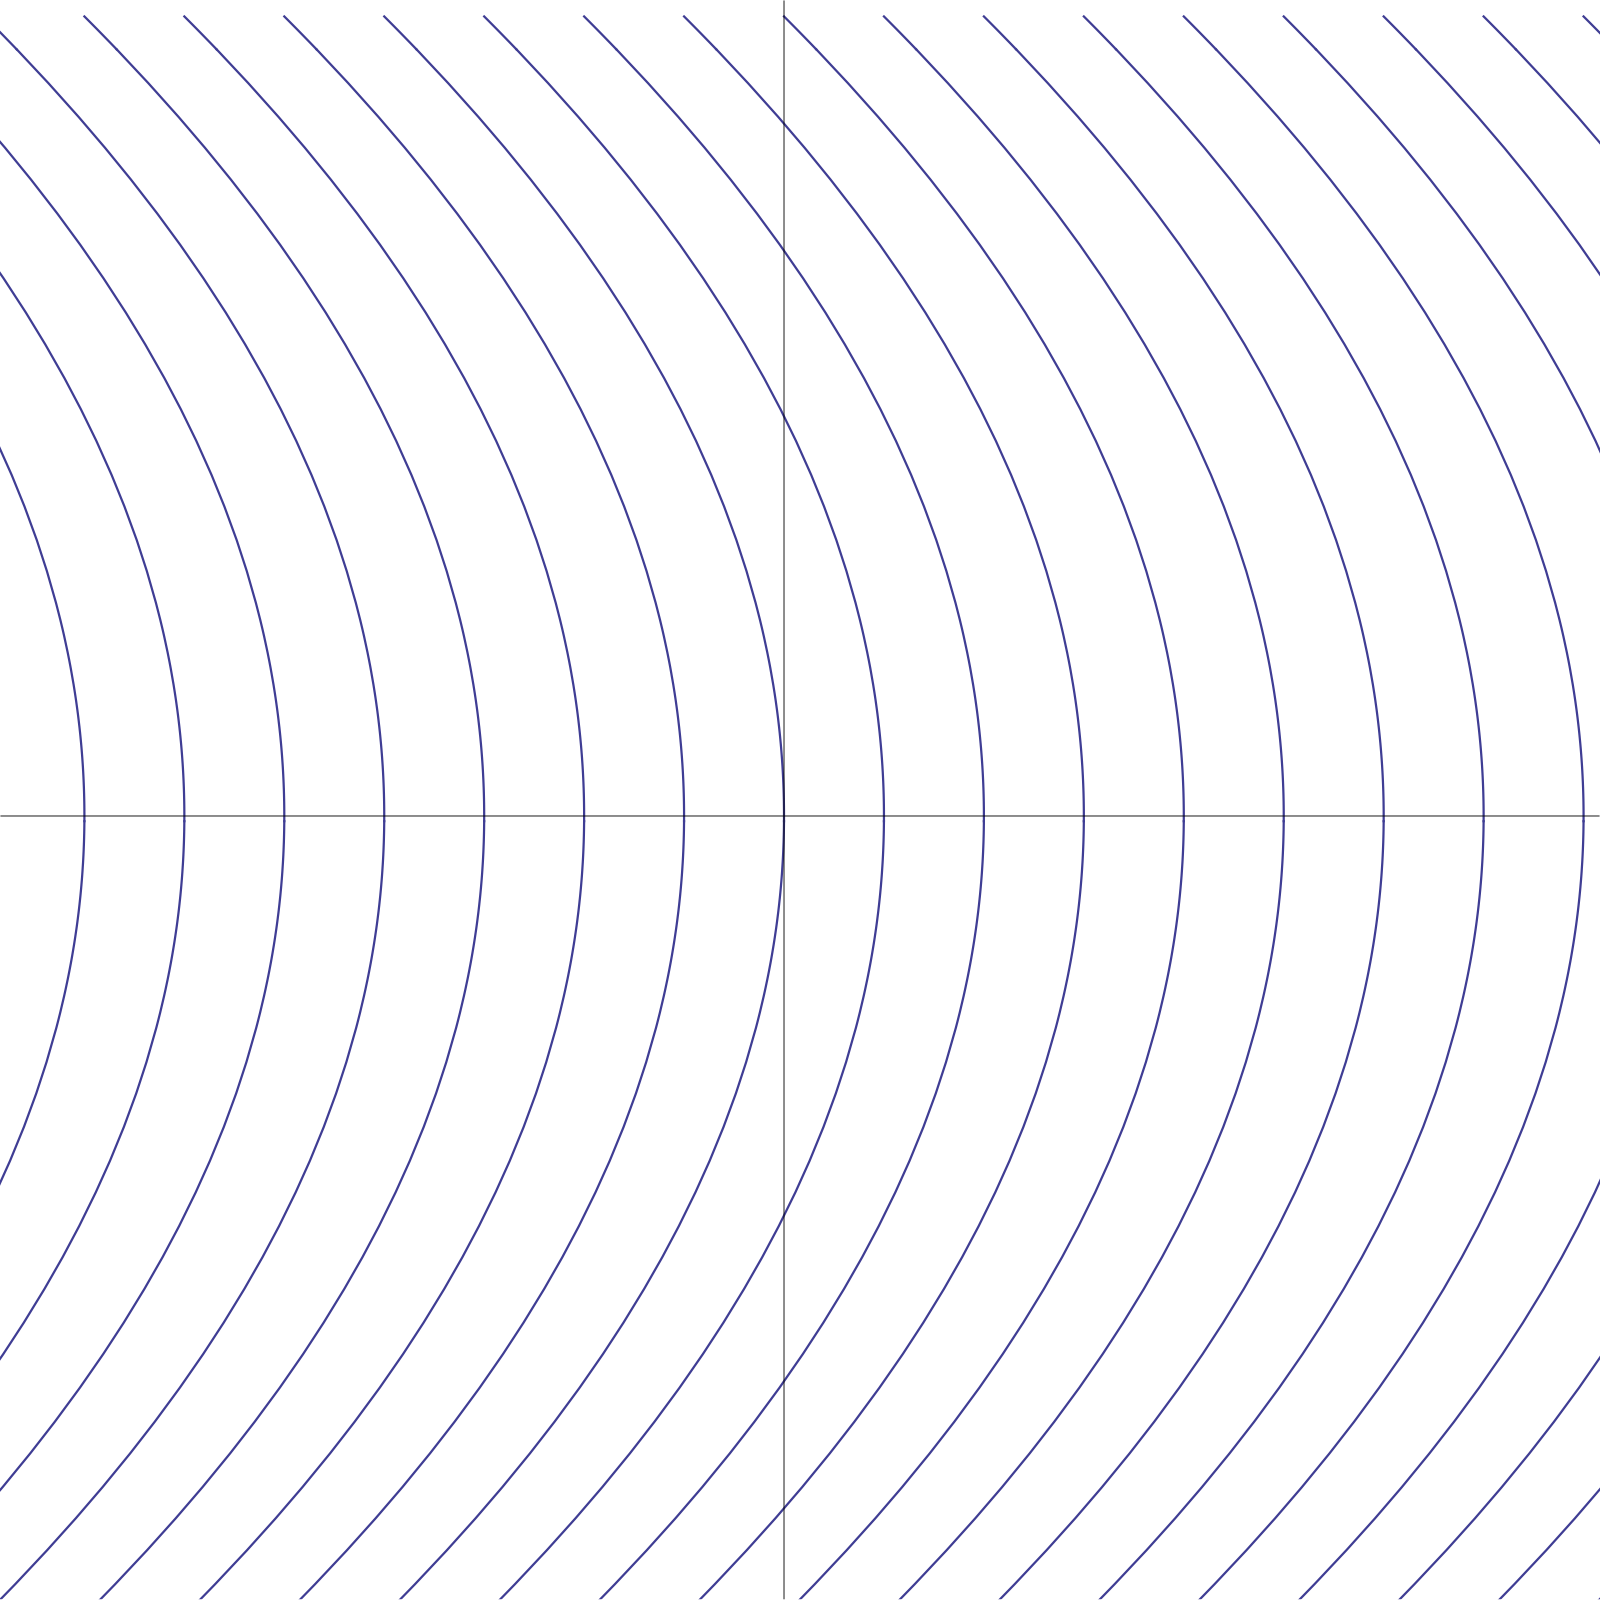
\includegraphics[width=0.55\linewidth]{figures/phasediag-gravity.png}\\[0.6em]
{\small Figure 14: The phase portrait for a particle falling
under the influence of gravity.}
\end{center}

\noindent Next, the system \eqref{eq:magnet-unstable} consists of
modifying the equation vector field by reflecting the
flow curves for negative $x$ so that they mirror the
lines for positive $x$. This leads to the phase
portrait in Figure 15. We see that the system indeed
has a rest point at $(x,y)=(0,0)$. However, the rest
point is a center, i.e., it is only neutrally stable
(this is to be expected, since in fact this is an
autonomous Hamiltonian system arising from a potential
energy $U(x)=|x|$, and we know energy is conserved in
such systems, leading to periodic oscillatory
motions). So, a particle moving according to these
equations of motion will indeed levitate, but will do
so in a way that oscillates around the reference point
$x=0$, and only under the unrealistic assumption that
the physical system is indeed described to perfect
precision by the equations \eqref{eq:magnet-unstable}. In
practice, due to the finite speed of response of the
switching control, any physical implementation of this
control rule will be unstable.

\begin{center}
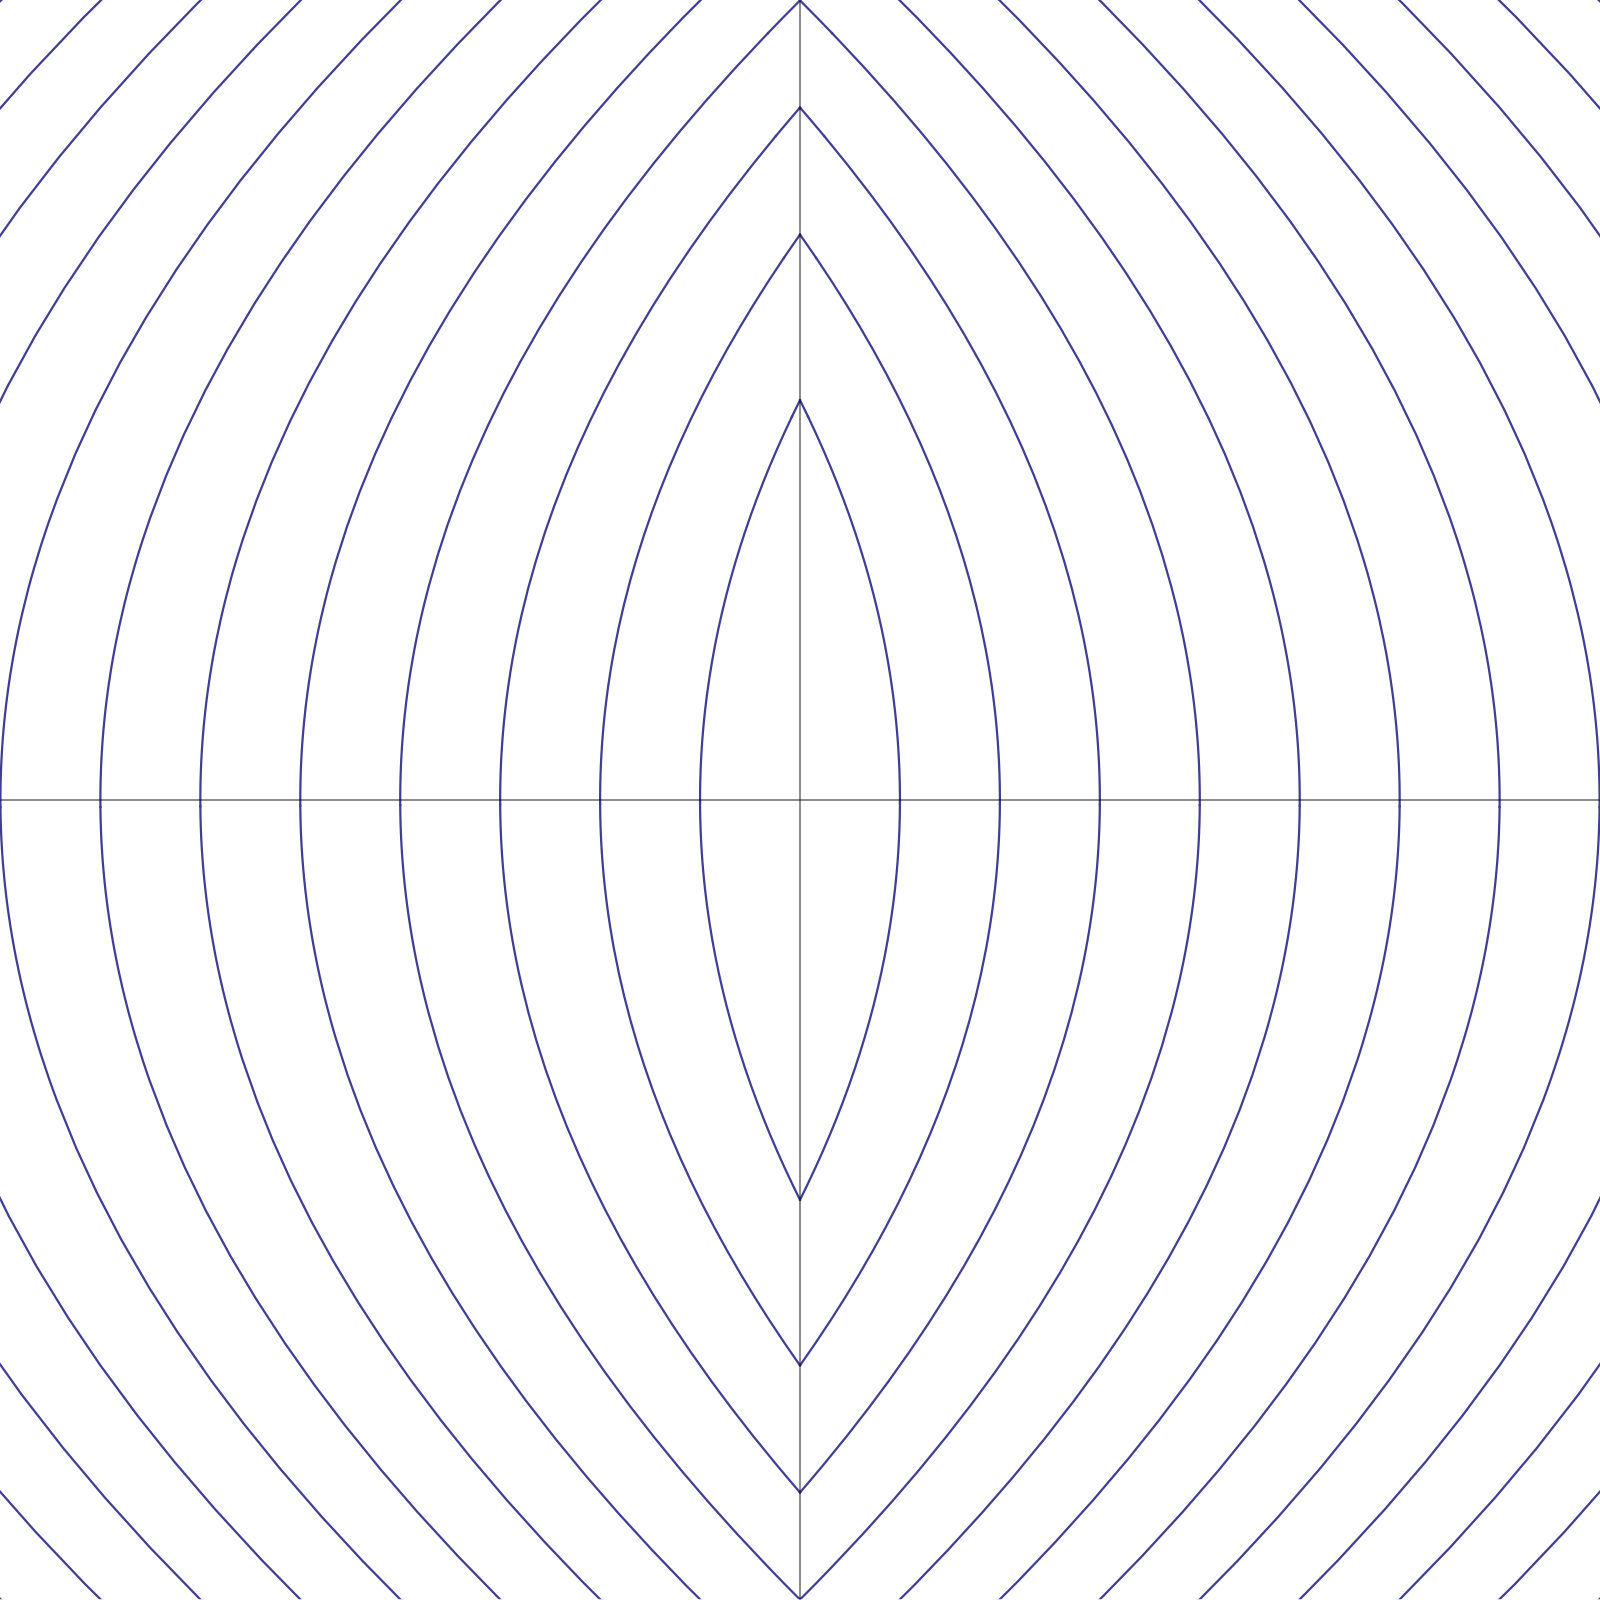
\includegraphics[width=0.55\linewidth]{figures/phasediag-magnet-unstable.png}\\[0.6em]
{\small Figure 15: The phase portrait for the equation of
motion of a magnetically levitated object, using the
``naive'' approach. The rest point is only neutrally
stable, and in practice this approach does not result
in stable levitation.}
\end{center}

\subsection{Taking velocity into account}

It is apparent that to achieve stable levitation, a
new idea is needed. Note that until now we only used
information about the position of the particle. Why
not use information about its velocity (the $y$
coordinate of the system's state $(x,\dot{x})$ when
represented as a planar system) as well? Intuitively,
this should help, since it's clear that the reason for
oscillations developing in the previous scheme is that
we are allowing the particle to overshoot the
equilibrium point from either direction before
toggling the state of the electromagnet; by looking at
the velocity we could predict where the particle will
be in a short time and do the toggling in advance in a
way that will gradually reduce the size of the
oscillations.

Formally, the idea described above leads to a
feedback rule of the type

\begin{align*}
u = -\operatorname{sgn}(x+b\dot{x}),
\end{align*}

\noindent where $b>0$ is a small numerical constant. This leads
to the modified system

\begin{align*}
\dot{x} = y, \quad \dot{y}= - \operatorname{sgn}(x+b y).
\end{align*}

\noindent To draw the phase portrait for the modified system,
again one has to combine the curves from the simple
gravity system \eqref{eq:gravity-system} with their mirror
images, but the choice of which one to draw at a given
point goes according to which side of the line
$x+by=0$ the point is on. Finding the intersection
points of the parabolas $x=a-\tfrac12 y^2$ and
$x=a+\tfrac12y^2$ with the line $x+by=0$ leads to
quadratic equations which are easily solved, so the
phase portrait can be plotted fairly easily. The
result is shown in Figure 16.

\begin{center}
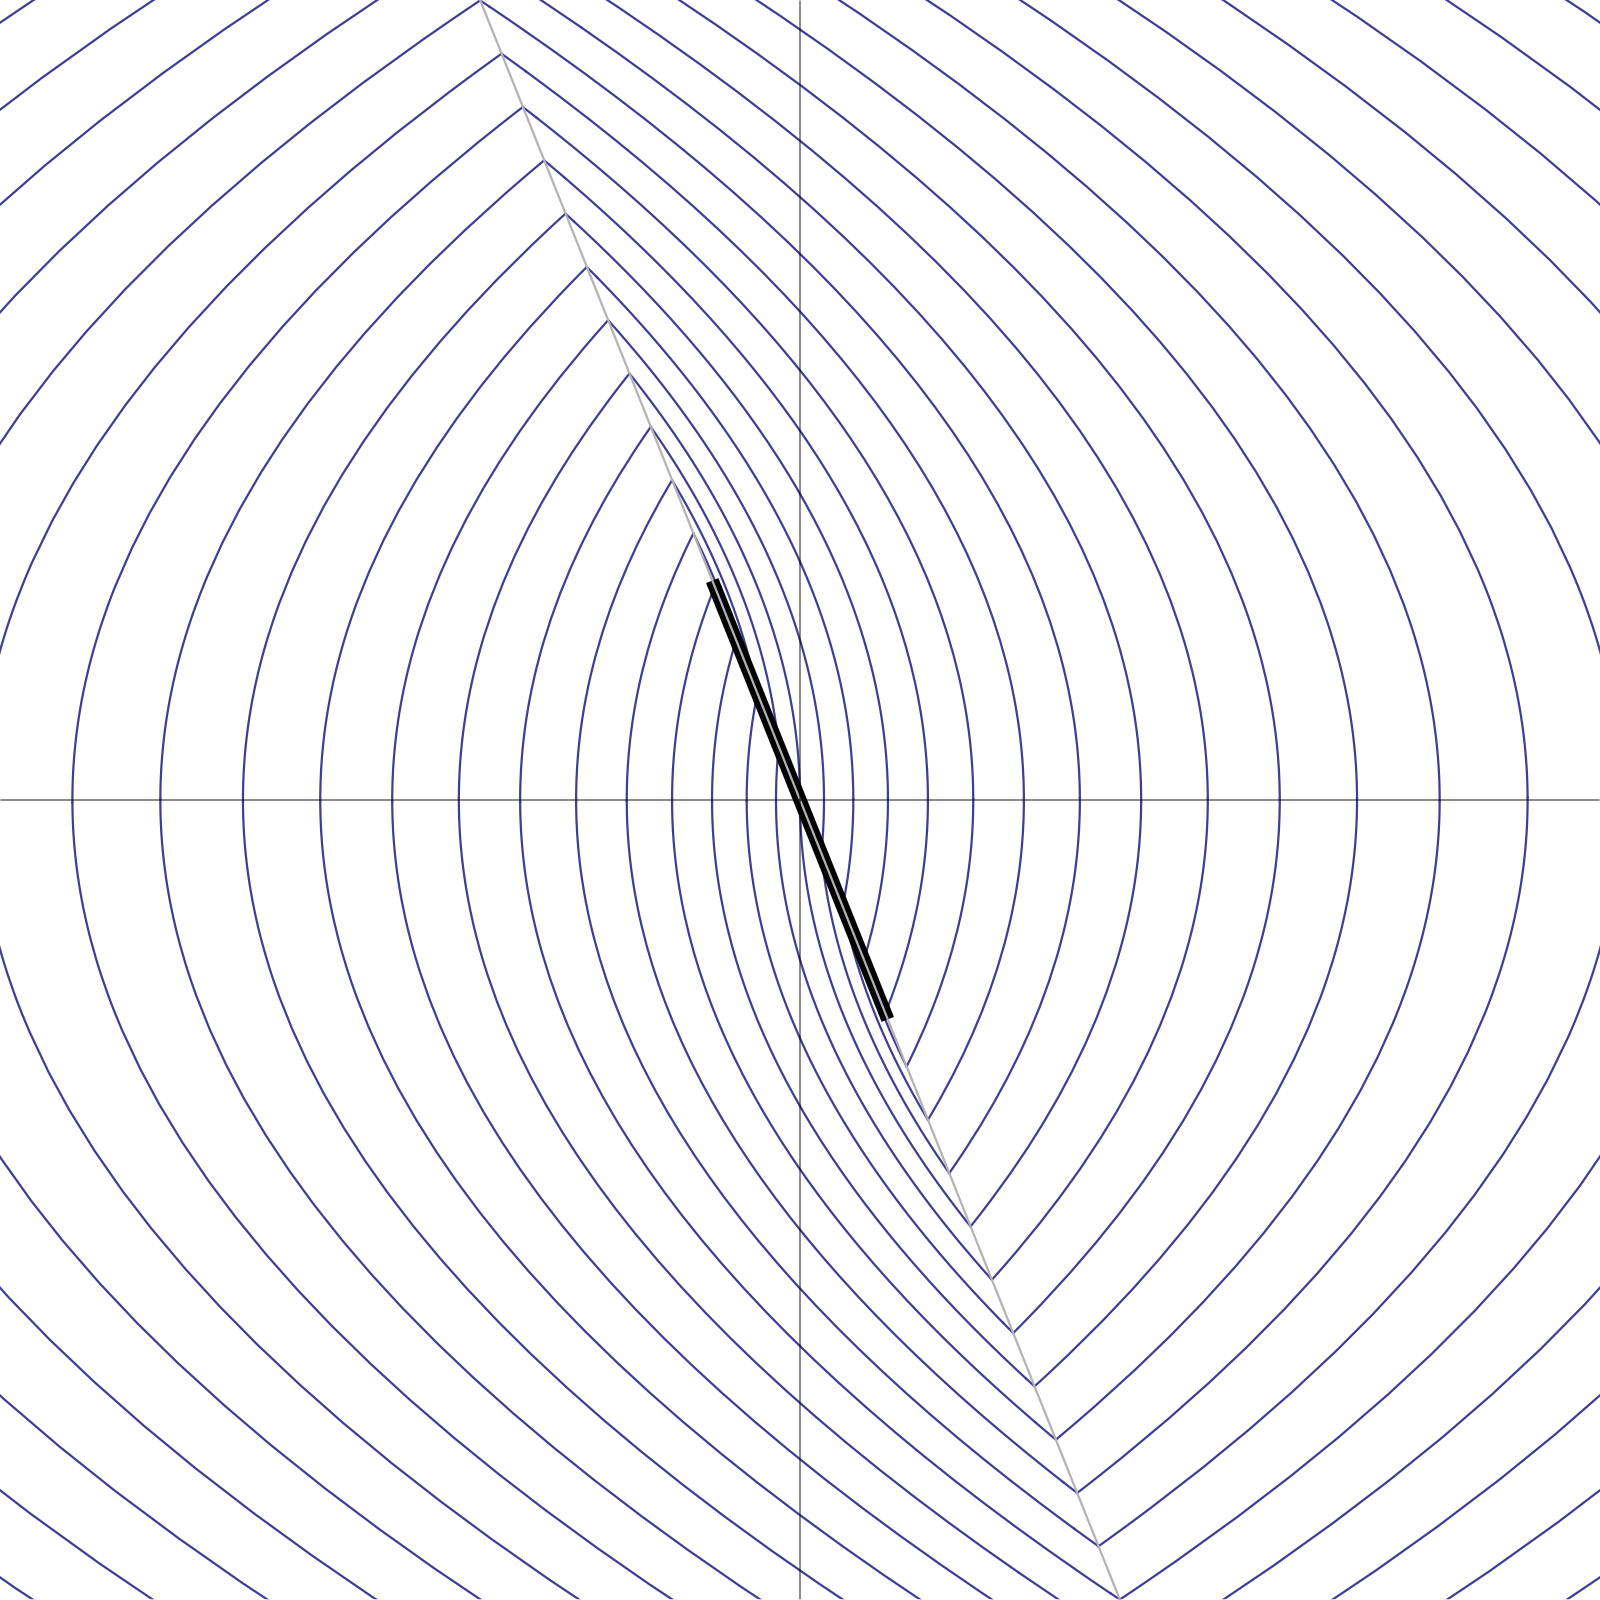
\includegraphics[width=0.55\linewidth]{figures/phasediag-magnet-stable.png}\\[0.6em]
{\small Figure 16: A feedback rule based on a linear
combination of position and velocity leads to stable
levitation. The final stage of the convergence to the
equilibrium point is a non-smooth ``sliding motion''
along a ``chattering curve'', shown in black.}
\end{center}

\noindent A look at the phase portrait suggests that the idea
is successful, and indeed results in stable
levitation. It is not difficult to confirm this
analytically. One interesting behavior that emerges
upon closer examination of the properties of this
system is that when $(x,y)$ crosses the switching
line $x+by=0$, if the point is close enough to the
origin then the equation of motion becomes
ill-defined, since the vector field
$(y,-\operatorname{sgn}(x+by))$ starts pointing back
towards the switching line. In practice, due to
time-delay effects in any physical implementation of
the system, the particle will undergo a ``sliding
motion'' in which it oscillates violently around both
sides of the switching motion, all the while still
sliding towards the origin. This phenomenon has been
referred to as \emph{chattering}, since in physical
implementations where the binary switching is done
using an electrical relay, the high frequency
switching makes a chattering noise. We can estimate
the rate at which the particle will approach the
origin during the sliding motion stage: since the
sliding motion happens very near the line $x+by=0$
and we have the equation $\dot{x}=y$, the particle's
position will approximately satisfy the ODE
$\dot{x}=-x/b$, whose solution is given by

\begin{align*}
x(t) = c e^{-t/b}.
\end{align*}

\noindent That is, the convergence to the origin in the final
sliding stage is exponential, with a time constant of
$1/b$.

\begin{xexercise}

\begin{enumerate}[label=\arabic*.]
\item Show that the sliding motion for points along the
line $x+by=0$ happens precisely for $|x|\le b^2$.

\item If we start the system at a point $(x_0,y_0)$ that
lies on the switching line $x+by=0$, find a formula
for the time it takes the point to flow into the
sliding motion area connecting the points $(-b^2,b)$
and $(b^2,-b)$.)
\end{enumerate}

\end{xexercise}

\subsection{Optimal switching control}

Although we have achieved our goal of designing a
stable levitation control scheme, it is not necessary
to stop here. A natural question is to ask for the
\emph{optimal} control rule, namely the one that causes the
particle to reach the stable equilibrium point in the
shortest time, regardless of its initial conditions.
Using ideas from the theory of nonlinear optimal
control which are beyond the scope of this course, it
is possible to prove that the optimal control rule is

\begin{align*}
u(x) = -\operatorname{sgn}\left(x+\tfrac12 \dot{x}|\dot{x}|\right).
\end{align*}

\noindent This makes intuitive sense, since the idea behind
this control rule is to toggle the electromagnet as
soon as the state of the system reaches the curve
$x=\tfrac12 y|y|$. The flow from that point on takes
place along the parabola $x=\tfrac12 y^2$ (if $x>0$)
or $x=-\tfrac12 y^2$ (if $x<0$) and leads directly to
the origin with no further toggling of the
controller's state required. The phase portrait of the
system governed by this control rule is shown in
Figure 17.

\begin{center}
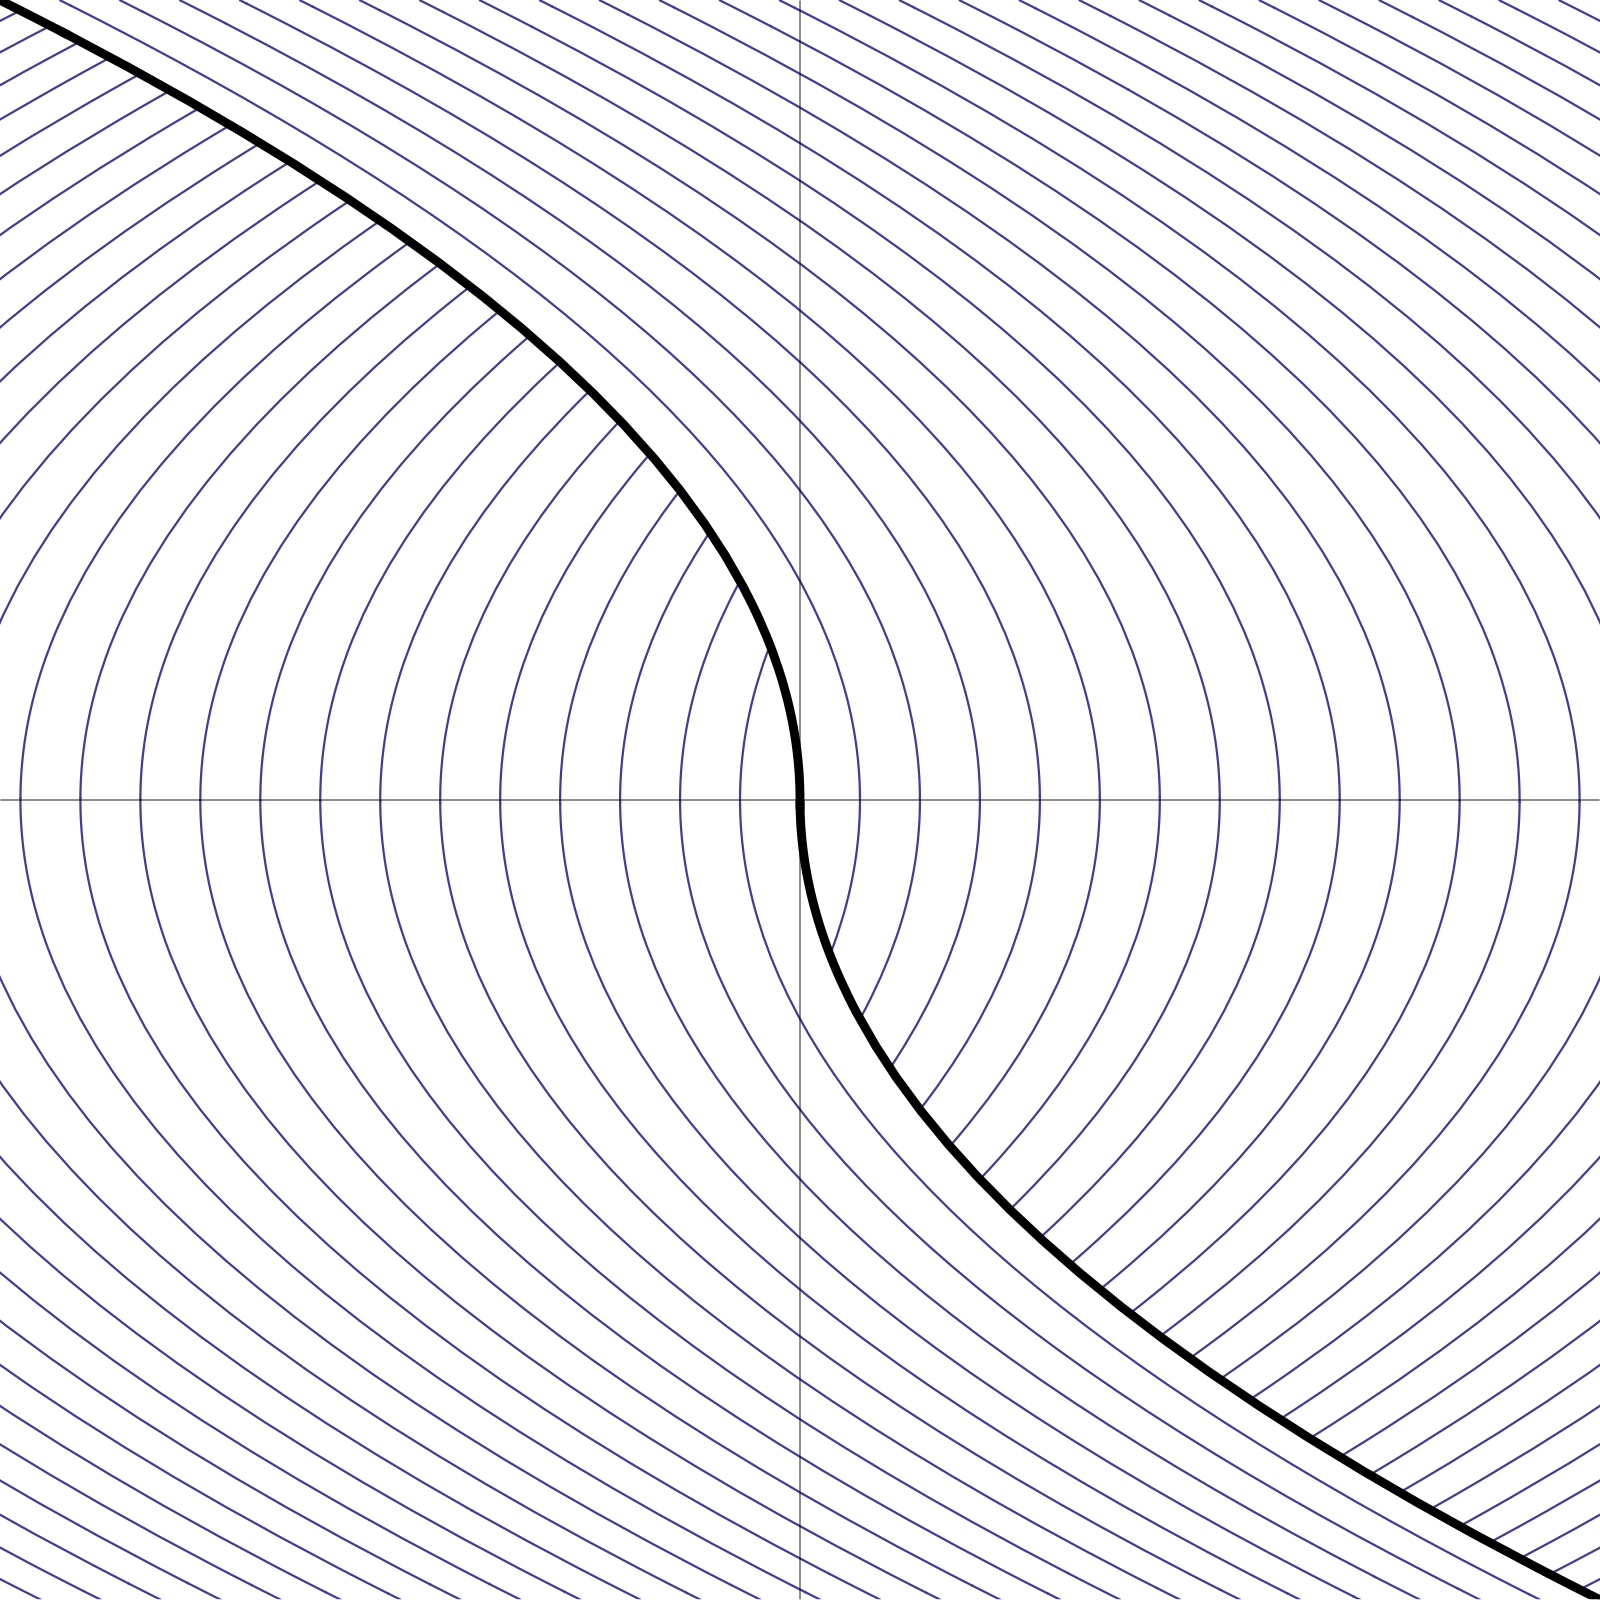
\includegraphics[width=0.55\linewidth]{figures/phasediag-magnet-optimal.png}\\[0.6em]
{\small Figure 17: Phase portrait for the optimal switching
control.}
\end{center}

\begin{xexercise}[Optimal switching time]
Find a formula for the time $\tau(x,\dot{x})$ it
takes the particle to get to the origin when the
optimal switching rule is used.
\end{xexercise}

\begin{center}
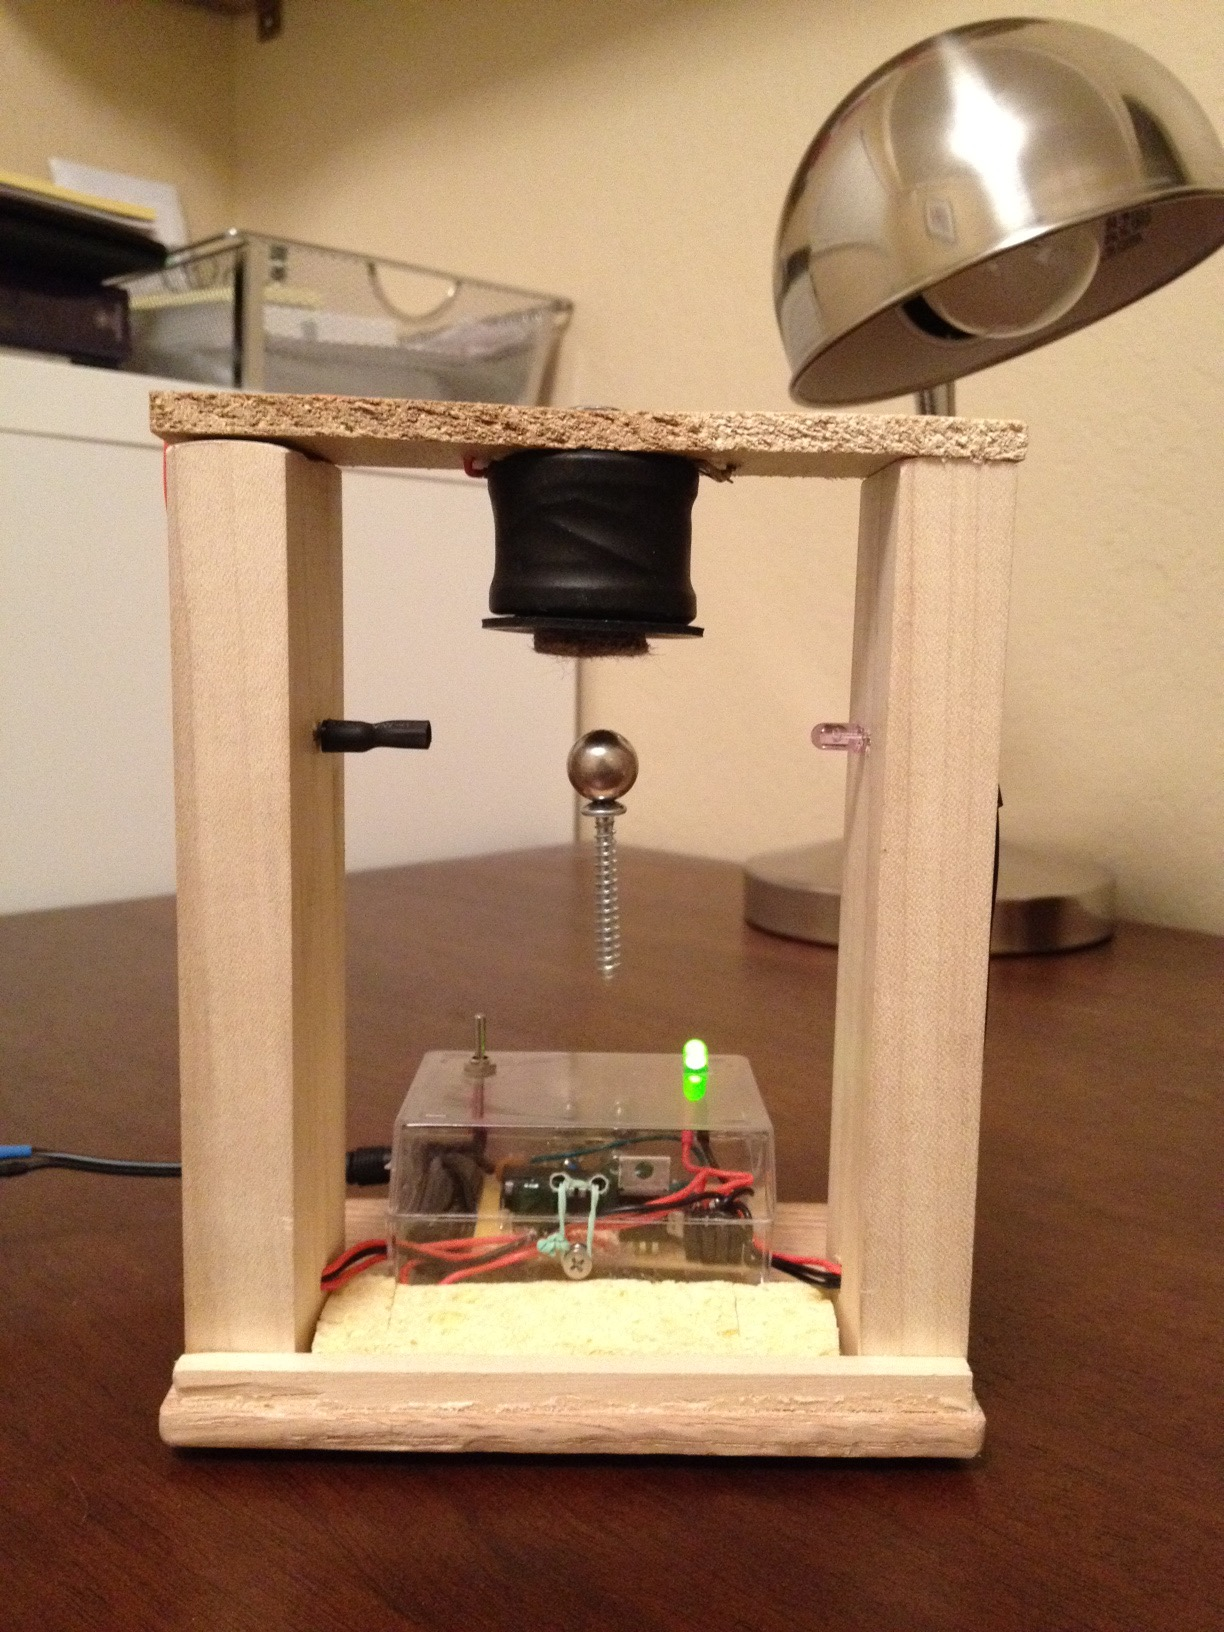
\includegraphics[width=0.45\linewidth]{figures/levitator1.jpg}\\[0.6em]
{\small Figure 18: A homemade electromagnetic levitation
device.}
\end{center}

\section{Linear Quadratic Performance control}

In this section we consider control problems which
take the general form

\begin{equation*} \tag{45}\label{eq:lqp-linear}
\begin{split}
\dot{\mathbf{x}} = A \mathbf{x} + B \mathbf{u},
\end{split}
\end{equation*}

\noindent where the state $\mathbf{x}$ of the dynamical system
is an $n$-dimensional vector, the control variable
$\mathbf{u}$ is an $m$-dimensional vector, and $A, B$
are linear operators (i.e., $A$ is an $n\times n$
matrix and $B$ is an $n\times m$ matrix). The goal of
the control will be to bring the dynamical variable
$\mathbf{x}$ to the origin. Moreover, we associate
with any proposed solution a \emph{cost functional} that
measures how effective it is. The cost functional will
take the form

\begin{equation*} \tag{46}\label{eq:lqp-quadratic}
\begin{split}
J = \int_{t_1}^{t_2}
\left( \mathbf{x}^\top P \mathbf{x} + \mathbf{u}^\top Q \mathbf{u} \right)\, dt,
\end{split}
\end{equation*}

\noindent where $-\infty<t_1<t_2\le \infty$, $P$ is an
$n\times n$ positive-definite matrix and $Q$ is an
$m\times m$ positive-definite matrix. The idea is
that we want to incentivize the controller to bring
$\mathbf{x}$ to the origin as fast as possible by
``pushing'' on it as hard as possible; at the same
time, in a typical situation the ``pushing'' also
incurs a price since it uses resources such as
electricity, fuel, etc. The problem of optimal control
is to find the feedback-based solution
$\mathbf{u}=\mathbf{u}(\mathbf{x})$ that minimizes
the overall cost functional, which finds a balance
between the cost of resources and the desire to
achieve good performance. It turns out that the
solution has the form

\begin{equation*} \tag{47}\label{eq:lqp-gain-mat}
\begin{split}
\mathbf{u} = -K \mathbf{x},
\end{split}
\end{equation*}

\noindent where $K$ is a time-dependent linear operator which
we will identify. Usually $K$ is expressed in the
form $K(t_2-t)$, i.e., as a function of the
``time-to-go'' variable $T=t_2-t$. The most
interesting case is that of an infinite time horizon:
$t_2=\infty$; in this case we look for a stationary
solution in which $K$ is a constant matrix, called
the \emph{gain matrix}.

Note that the mapping that takes a pair
$(\mathbf{u},\mathbf{a})$ where $\mathbf{u}$ is the
control function and $\mathbf{a}$ is the initial
condition $\mathbf{x}(t_1)=\mathbf{a}$ to the
solution of \eqref{eq:lqp-linear} is linear, and the cost
functional \eqref{eq:lqp-quadratic} is a quadratic
expression in $\mathbf{x}$ and $\mathbf{u}$. Thus
this type of problem is referred to as Linear
Quadratic Performance (LQP) control. The main
advantage of LQP control problems is that they have an
explicit solution in terms of an ordinary differential
equation, the Ricatti equation, which furthermore is
easy to solve numerically.

\subsection{The one dimensional LQP control problem}

Since the problem in this generality is somewhat
complicated to analyze, to illustrate the main ideas
we will focus on a simple one-dimensional settting in
which $m=n=1$, the differential equation becomes

\begin{align*}
\dot{x} = ax+bu
\end{align*}

\noindent for some constants $a,b\in\mathbb{R}$, and the cost
functional takes the form

\begin{align*}
I = \int_{t_1}^{t_2} (px^2+qu^2)\,dt
\end{align*}

\noindent for some numbers $p,q>0$. Note that, for a given
control rule, to compute $I$ all that one needs to
know is the initial condition $x(t_1)$ and the
duration $T=t_2-t_1$ over which the cost is
integrated (that is, changing the left endpoint $t_1$
of the interval $[t_1,t_2]$ while keeping its length
fixed will not change the cost functional). Let
$I_*(w,T)$ denote the optimal control cost associated
with an initial condition $x(t_1)=w$ and an interval
$[t_1,t_2]$ of length $T$:

\begin{align*}
I_*(w,T) = \min_{\textrm{control rule $u$}} \int_{t_1}^{t_1+T} (p x^2+qu^2)\,dt
 \qquad (x(t_1)=w).
\end{align*}

\noindent In the derivation that follows, we assume that
$t_2<\infty$ and that $I_*(w,T)$ is a smooth function
of $w$ and $T$. Furthermore, it is not hard to see
due to the quadratic nature of $I$ that the
dependence of $I_*(w,T)$ on $w$ is also quadratic,
i.e., we can write

\begin{align*}
I_*(w,T) = v(T) w^2
\end{align*}

\noindent for some smooth function $v(T)$. The variable
$T=t_2-t_1$ is nonnegative, and for $T=0$ we clearly
have $v(0)=0$.

Now, let $\delta$ be a small positive number. We
separate the interval $[t_1,t_2]$ into the
subintervals $[t_1,t_1+\delta]$ and
$[t_1+\delta,t_2]$. When optimal control is used for
the entire interval $[t_1,t_2]$, in particular the
control rule for each subinterval is also optimal.
Thus, we have the equation

\begin{equation*} \tag{48}\label{eq:lqp-subintervals}
\begin{split}
I_*(w,T) = I_*(w,\delta) + I_*(z,T-\delta),
\end{split}
\end{equation*}

\noindent where $z=x(t_1+\delta)$ is the value obtained from
the solution of the optimal control problem with
initial condition $x(t_1)=w$ for the interval
$[t_1,t_1+\delta]$. When $\delta$ is small, we have
the following linear approximations in $\delta$:

\begin{equation*} \tag{49}\label{eq:lqp-approx}
\begin{split}
I_*(w,\delta) &= (p w^2 + q u_*^2)\delta + O(\delta^2), \\
z &= w + \dot{x}(0)\delta + O(\delta)^2 = w + (aw+b u_*)\delta + O(\delta^2),
\end{split}
\end{equation*}

\noindent where $u_*$ is the value of the control variable at
time $t=t_1$ when optimal control is used with
initial condition $x(t_1)=w$ over the interval
$[t_1,t_2]$. Note that like $I_*$, $u_*$ depends only
on $w$ and $T=t_2-t_1$. Furthermore, by dimensional
considerations, the dependence of $u_*$ on $w$ is
linear, so we may write

\begin{align*}
u_* = - k(T)w.
\end{align*}

\noindent The scalar quantity $k(T)$ is a gain factor,
analogous to the operator $K$ mentioned above in
connection with the LQP control problem in arbitrary
dimension.

Now, continuing \eqref{eq:lqp-subintervals}, we may
further expand all terms on the right-hand side as
linear approximations in $\delta$:

\begin{align*}
I_*(w,T) &= I_*(w,\delta) + I_*(z,T-\delta) \\
&= (p w^2 + q u_*^2)\delta \\ & \qquad +
I_*(w,T) + \frac{\partial I_*}{\partial w}(w,T)(z-w) + \frac{\partial I_*}{\partial T}(w,T)(-\delta) + O(\delta^2) \\
&=
I_*(w,T) + \delta\left[
(p w^2+qu_*^2) + 2w v(T)(aw+b u_*) - v'(T) w^2
\right] \\
& \qquad + O(\delta^2).
\end{align*}

\noindent In the limit when $\delta\downarrow 0$ we therefore
get that

\begin{align*}
(p w^2+qu_*^2) + 2w v(T)(aw+b u_*) - v'(T) w^2 = 0,
\end{align*}

\noindent or, substituting $-k(T)w$ for $u_*$, we have the
equation

\begin{align*}
w^2\left(
p + q k^2 + 2av(T) -2 b k v(T) -v'(T)
\right) = 0,
\end{align*}

\noindent where we write $k$ instead of $k(T)$. Since $w$ is
arbitrary, we get the relation

\begin{equation*} \tag{50}\label{eq:lqp-quadratic-poly}
\begin{split}
p + q k^2 + 2av(T) -2 b k v(T) -v'(T) = 0.
\end{split}
\end{equation*}

\noindent We still don't know $k$ (or equivalently, $u_*$); but
now, recalling that $u_*$ was defined from the value
of the control variable \emph{under optimal control}, we
see that the left-hand side of
\eqref{eq:lqp-quadratic-poly}, which is a quadratic
polynomial in $k$, must take its minimum at the
correct value $k=k(T)$:

\begin{align*}
k &= \textrm{value of $s$ for which }\  qs^2-2b v(T) s + p-v'(T)\ \textrm{ is minimized} \\
&= \frac{b v(T)}{q}.
\end{align*}

\noindent (Recall that a quadratic polynomial $a_2s^2+a_1s+a_0$
has its extremum point when $s=-a_1/2a_2$, as can be
seen by equating its derivative to $0$).

Summarizing, we have found that the unknown gain
function $k(T)$ is given by $k(T) = b v(T)/q$, where
$v(T)$, heretofore also unknown, is the solution of
the differential equation

\begin{equation*} \tag{51}\label{eq:lqp-ricatti1}
\begin{split}
v'(T) = p + 2 a v(T) - \frac{b^2}{q} v(T)^2
\end{split}
\end{equation*}

\noindent obtained by plugging the expression for $k(T)$ back
into \eqref{eq:lqp-quadratic-poly}, with the initial
condition $v(0)=0$. This is the \emph{Ricatti equation
with constant coefficients}.

\subsection{The case of an infinite time horizon}

The case $t_2=\infty$ can be approached by letting
$T\to\infty$ in the equation above. The solution
$v(T)$ of the Ricatti equation should converge to a
stationary point satisfying $v'(T)=0$, so we get for
this case that the limiting value $v_\infty$ of $v(T)$
must satisfy the quadratic equation

\begin{align*}
v_\infty^2 - \frac{2aq}{b^2} v_\infty - \frac{pq}{b^2} = 0,
\end{align*}

\noindent giving that

\begin{align*}
v_\infty = \frac{aq}{b^2}\left( 1 \pm \sqrt{1+\frac{pb^2}{qa^2}}\right).
\end{align*}

\noindent Since we know that $v_\infty\ge 0$ and $p,q>0$, it
can be checked that the correct choice of sign is:

\begin{align*}
v_\infty = \begin{cases}
\frac{aq}{b^2}\left( 1 - \sqrt{1+\frac{pb^2}{qa^2}}\right)
&
\textrm{if }a<0,  \\
\frac{aq}{b^2}\left( 1 + \sqrt{1+\frac{pb^2}{qa^2}}\right)
&
\textrm{if }a>0.
\end{cases}
\end{align*}

\noindent The optimal control gain $k=k_\infty$ is then given
as before by $k_\infty = b v_\infty/q$. Note that the
case $a<0$ corresponds to a situation in which the
object is stable even in the absence of a control
force, i.e., if we take $u=0$.

\subsection{Generalization to arbitrary dimension}

By repeating the above analysis in a careful manner
for the general LQP problem in arbitrary dimension
discussed at the beginning of this section, one can
derive the solution for that general case. For the LQP
problem with a finite horizon, the gain matrix $K(T)$
from \eqref{eq:lqp-gain-mat} is expressed as a matrix
product

\begin{align*}
K(T) = Q^{-1}B^\top V(T),
\end{align*}

\noindent where $V(T)$ is a matrix related to the optimal cost
function $J_*(\mathbf{w},T)$ (defined analogously to
$I_*(w,T)$) by

\begin{align*}
J_*(\mathbf{w},T) = \mathbf{w}^\top V(T)\mathbf{w}.
\end{align*}

\noindent Furthermore, $V$ satisfies the matrix differential
equation (also referred to as the Ricatti equation)

\begin{align*}
\frac{dV}{dt} = P + A^\top V(T) + V(T) A - V(T) B Q^{-1} B^\top V(T)
\end{align*}

\noindent with boundary condition $V(0) = 0$ (the zero matrix).
For an infinite time horizon, we again look for
stationary solutions, which leads to the \emph{algebraic
Ricatti equation}

\begin{align*}
P + A^\top V + V A - V B Q^{-1} B^\top V = 0,
\end{align*}

\noindent which is a system of quadratic equations in the
entries of $V$. The (constant) gain matrix $K$ is
again given by

\begin{align*}
K = Q^{-1}B^\top V.
\end{align*}

\noindent While these equations may seem intimidating at first
sight, they are easy to solve numerically on a
computer. Symbolic math software applications such as
$\texttt{Mathematica}$ even contain specialized
packages for control theory that make the process of
deriving optimal LQP control rules highly automated
and quite simple in practice, as the next example
demonstrates.

\begin{example}[The inverted pendulum with cart: LQP optimal control with $\texttt{Mathematica}$]
The controlled inverted pendulum with cart is a
dynamical system with 2 degrees of freedom
$\theta=\theta(t)$ (representing the angle of the
pendulum relative to the positive $x$-axis) and
$x=x(t)$ (representing the displacement of the cart
along the $x$-axis), satisfying the equations of
motion\footnote{This example is based on a blog post written by
Andrew Moylan on the website of Wolfram Research
(maker of the $\texttt{Mathematica}$ software); see
the link:
\href{http://blog.wolfram.com/2011/01/19/stabilized-inverted-pendulum/}{http://blog.wolfram.com/2011/01/19/stabilized-inverted-pendulum/}}

\begin{align*}
4\ddot{x} &=  \ddot{\theta}\sin \theta + \dot{\theta}^2 \cos \theta + 2 u, \\
0 &= \ddot{\theta}+2\cos \theta - 2\ddot{x} \sin\theta,
\end{align*}

\noindent where $u$ is the control variable representing a
control force being applied to the cart --- see Figure
19.

\begin{center}
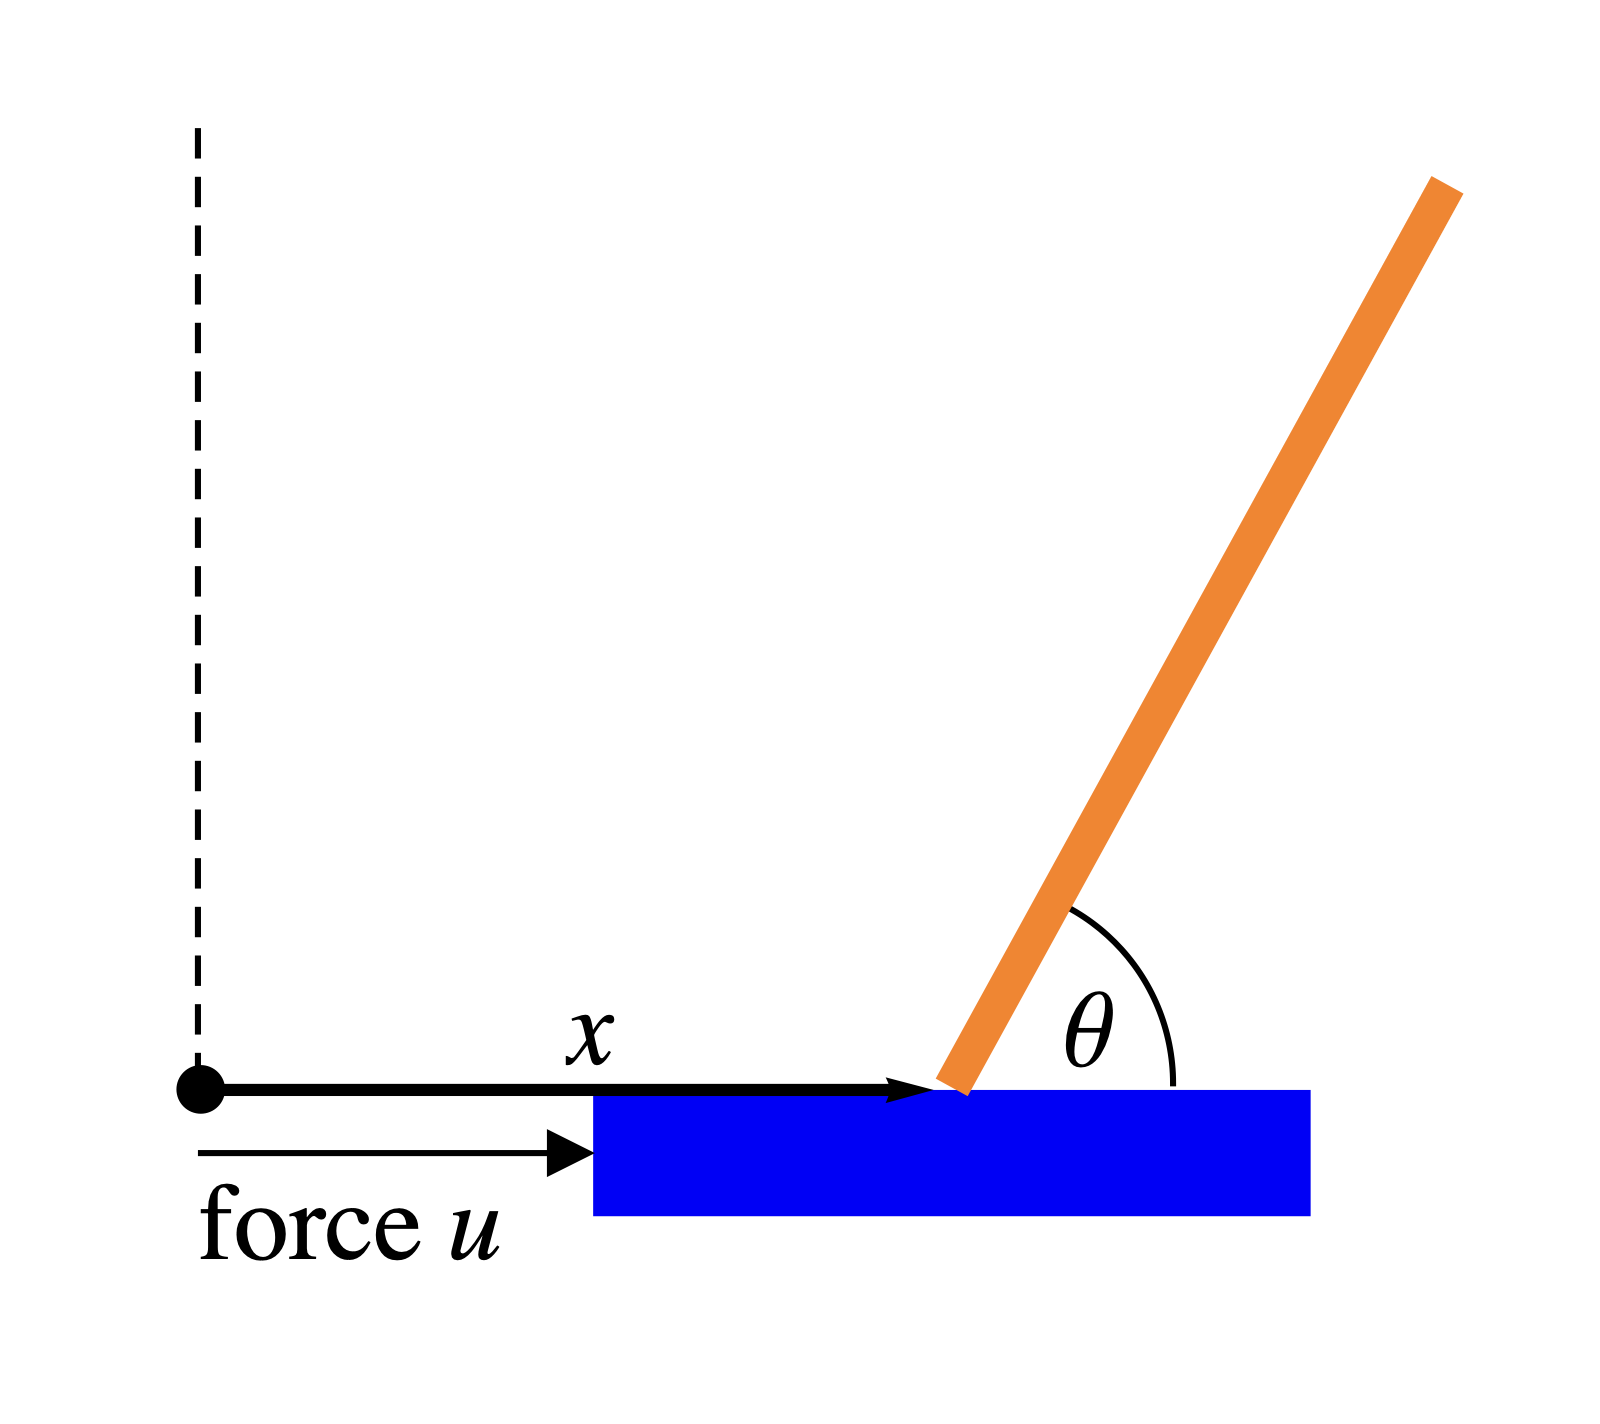
\includegraphics[width=0.48\linewidth]{figures/invertedpendulum-cart.png}\\[0.6em]
{\small Figure 19: The inverted pendulum and cart.}
\end{center}

\noindent The system can be thought of in the usual way as a
system of 4 coupled first-order ODEs in the variables
$\theta, \dot{\theta}, x, \dot{x}$. The goal of the
control problem is to bring the system to a stable
equilibrium at
$(x,\dot{x},\theta,\dot{\theta}) = (0,0,\pi/2,0)$. In
$\texttt{Mathematica}$, we type the following
commands:

\begin{align*}
\scriptsize{\text{In[1]=}}\quad & \text{eqns}=\left\{2 u[t]+\text{Cos}[\theta [t]] \theta '[t]^2+\text{Sin}[\theta [t]] \theta ''[t]==4 x''[t], \right.\\ & \qquad\qquad \qquad  \qquad \left. 2 \text{Cos}[\theta [t]]-2 \text{Sin}[\theta [t]] x''[t]+\theta ''[t]==0\right\};
\\
\scriptsize{\text{In[2]=}}\quad &\text{model}=\text{StateSpaceModel}\Big[\text{eqns}, \\ & \qquad\qquad \left\{\{x[t],0\},\{x'[t],0\},\left\{\theta [t],\frac{\pi }{2}\right\},\{\theta '[t],0\}\right\},u[t],\{\},t\Big]
\\
\scriptsize{\text{Out[2]=}}\quad &
\left(
\begin{array}{cccc|c}
0 & 1 & 0 & 0 & 0 \\
0 & 0 & 1 & 0 & 1 \\
0 & 0 & 0 & 1 & 0 \\
0 & 0 & 4 & 0 & 2 \\
\end{array}
\right)_{}^{\mathcal{S}}
\end{align*}

\noindent The second command causes $\texttt{Mathematica}$ to
linearize the equations of motion around the desired
rest point. The output is an augmented matrix of the
form $\left( A\,|\,B\right)$ where $A, B$ are the two
matrices in the resulting linearized equation
\eqref{eq:lqp-linear}. This brings the problem to the
familiar setup of LQP optimal control which we
discussed above. We now type:

\begin{align*}
\scriptsize{\text{In[3]=}}\quad &
\text{gains}=\text{LQRegulatorGains}[\text{N}[\text{model}], \\
& \qquad\qquad
\{\text{DiagonalMatrix}[\{1,10,10,100\}],\{\{1\}\}\}]\text{//}\text{First}
\\
\scriptsize{\text{Out[3]=}}\quad &
\{-1.,-5.97415,14.8452,13.7966\}
\end{align*}

\noindent This asks $\texttt{Mathematica}$ to compute the gain
matrix $K$ (in this case a vector with 4 coordinates)
associated with the cost functional
\eqref{eq:lqp-quadratic} (in the case $t_2=\infty$ of an
infinite time horizon), where the quadratic forms
$P, Q$ are defined by

\begin{align*}
P = \left(\begin{array}{cccc}
1&0&0&0\\0&10&0&0\\0&0&100&0\\0&0&0&1000
\end{array}\right),
\qquad
Q = (1).
\end{align*}

\noindent Using the gain matrix computed by
$\texttt{Mathematica}$, we see that the solution to
the optimal control problem we defined is given by the
feedback rule

\begin{align*}
u = - x -5.97415\, \dot{x} + 14.8452\, \theta + 13.7966\, \dot{\theta}.
\end{align*}

\end{example}

\chapter*{Bibliographic notes}
\addcontentsline{toc}{chapter}{Bibliographic notes}
Here are the main sources I used during the preparation of these lecture notes. I had a lot of fun consulting these books, but had to leave out many beautiful topics. The interested reader is encouraged to continue his or her journey into the world of ODEs by looking into these more detailed sources. I especially recommend the books by Arnold, Banks and anything written by Richard Feynman (including his hilarious memoir \emph{Surely You're Joking, Mr. Feynman}).

\textbf{Sources for Part 1}

\begin{enumerate}[label=\arabic*.]
\item V. I. Arnold, Mathematical Methods of Classical Mechanics, 2nd Ed. Springer, 1988.

\item R. B. Banks, Towing Icebergs, Falling Dominoes, and Other Adventures in Applied Mathematics. Princeton University Press, 1998.

\item R. Grimshaw, Nonlinear Ordinary Differential Equations. Blackwell Scientific Publications, 1990.

\item J. K. Hunter, \href{http://www.math.ucdavis.edu/~hunter/m280_09/applied_math.html}{Lecture Notes on Applied Mathematics}, available online.

\item L. A. Pars, An Introduction to the Calculus of Variations. Heinemann Educational Books, 1962 (reprinted by Dover Publications, 2010).
\end{enumerate}

\noindent \textbf{Sources for Part 2}

\begin{enumerate}[label=\arabic*., start=6]
\item D. Romik, Lecture Notes for Math 235B: Probability Theory, available online at \href{http://www.math.ucdavis.edu/~romik/teaching/mat235-2011-2012/\#235b}{http://www.math.ucdavis.edu/~romik/teaching/mat235-2011-2012/\#235b}

\item S. H. Strogatz, Nonlinear Dynamics and Chaos. Westview Press, 1994.
\end{enumerate}

\noindent \textbf{Sources for Part 3}

\begin{enumerate}[label=\arabic*., start=8]
\item Chapter 5 of Arnold's book listed above.

\item R. P. Feynman, R. B. Leighton, M. Sands, The Feynman Lectures on Physics, Vol. II. Basic Books, 1964. (Chapter 29 has a discussion of alternating-gradient focusing and the inverted pendulum with an oscillating base.)

\item O. L. R. Jacobs, Introduction to Control Theory. Oxford Science Publications, 1993.
\end{enumerate}

\end{document}
